\chapter{Results}




\begin{figure}%
    \centering
    \subfloat[A cumulative measurement of $^{188}$Ir isomer and ground state, and beta-feeding feeding from $^{188}$Pt (100\%)]{{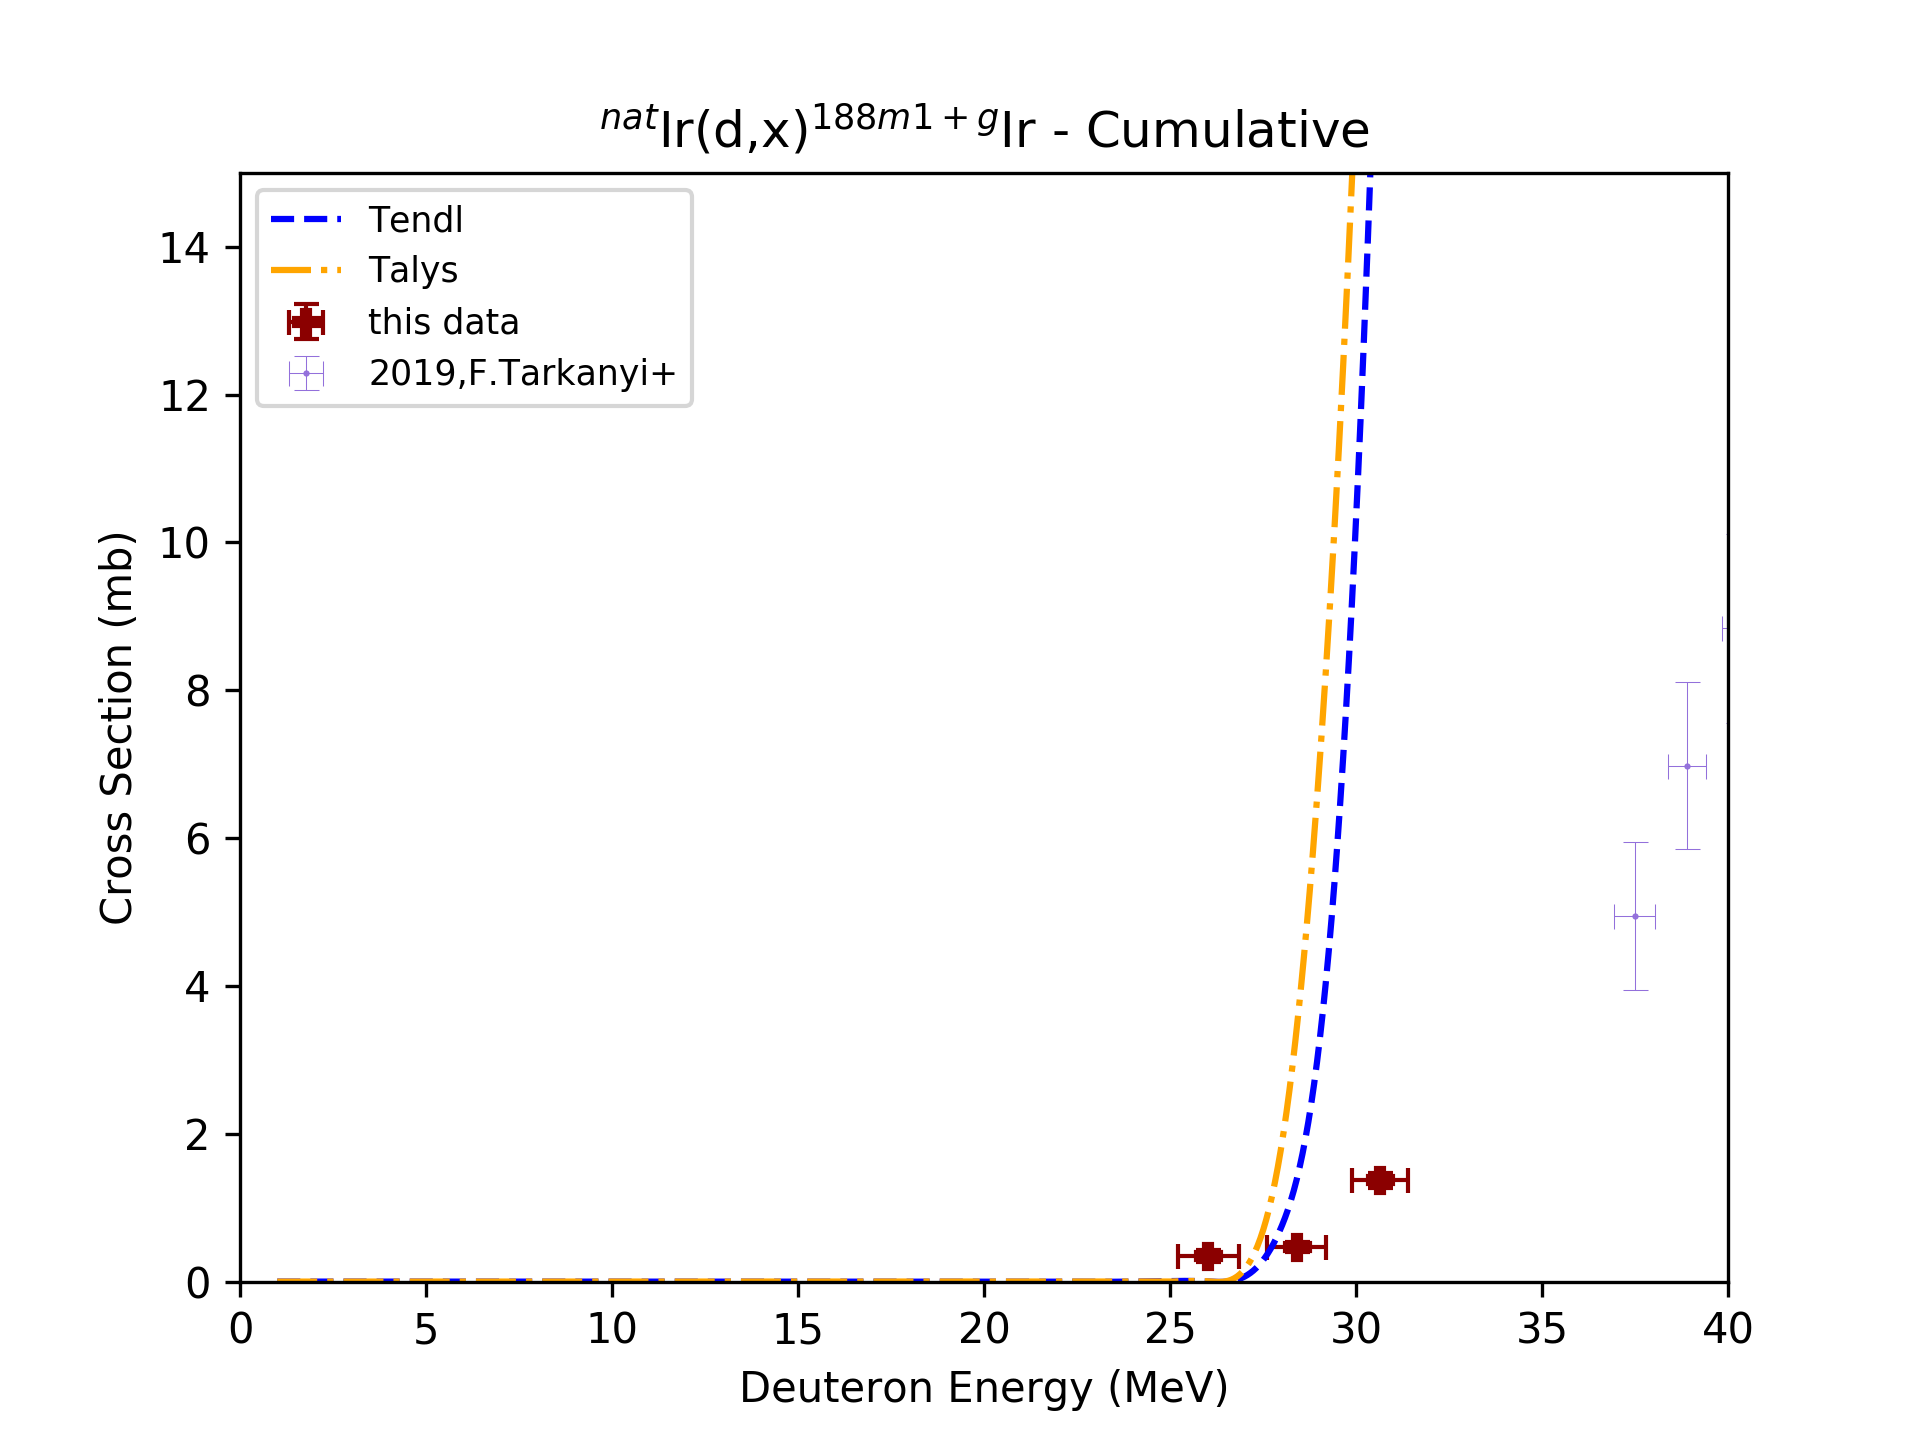
\includegraphics[width=8cm]{Results/Ir_188Ir.png} }}%
    \quad
    \subfloat[An independent measurement of the cumulative cross section for $^{188}$Ir isomer and ground state, with subtraction of the feeding-weighted percentage of $^{188}$Pt from the cumulative cross section. ]{{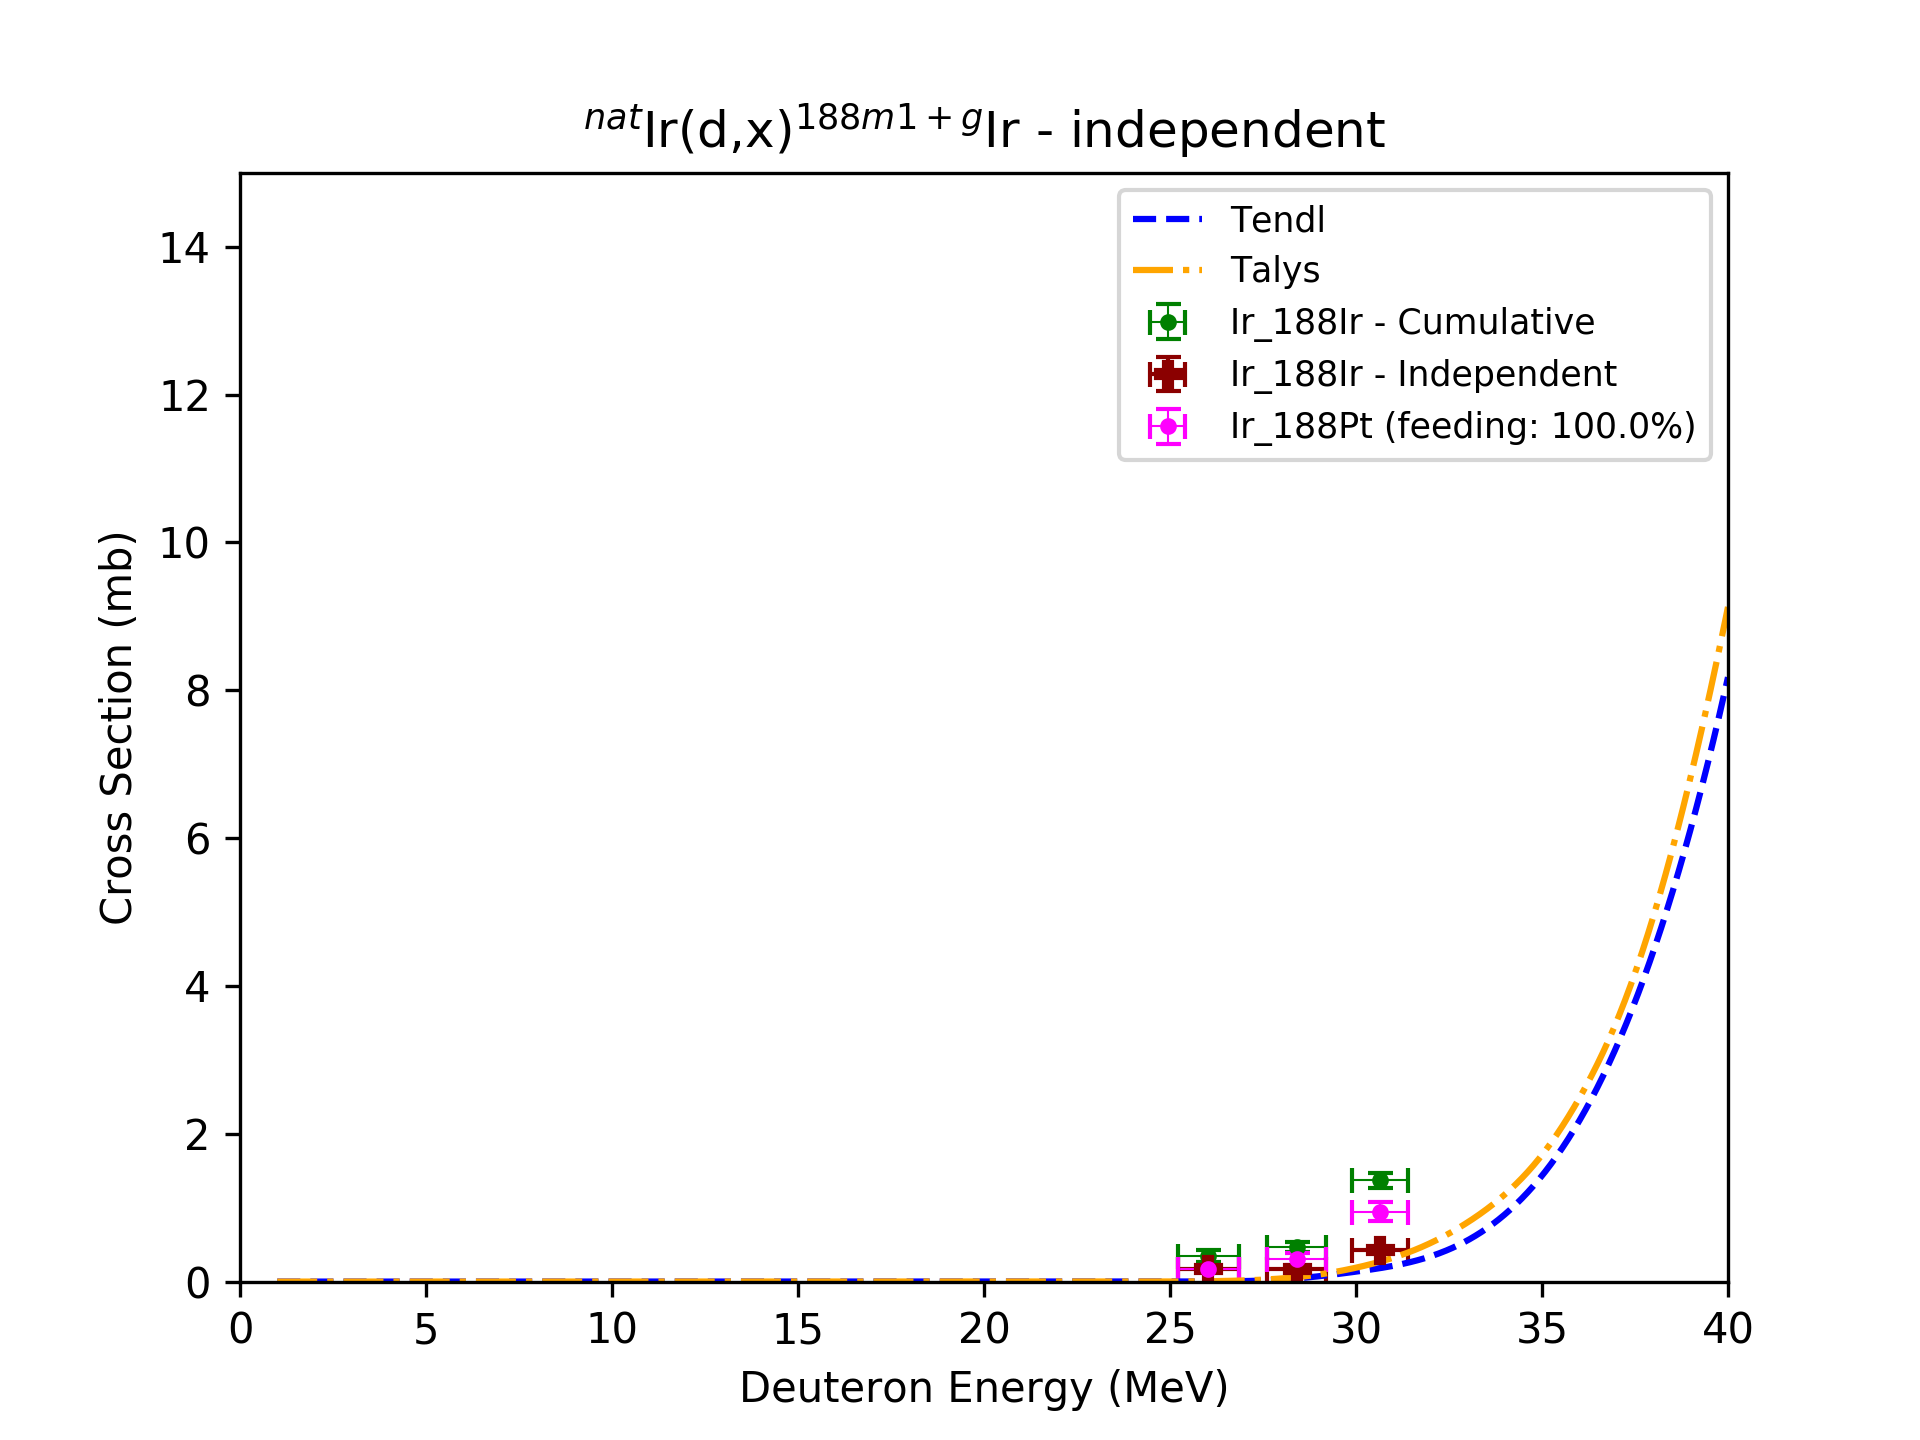
\includegraphics[width=8cm]{Results/Ir_188Ir_subtracted.png} }}%
    \quad
    \subfloat[A cumulative measurement of $^{189}$Ir isomers and ground state, and beta-feeding from $^{189}$Pt (100\%).]{{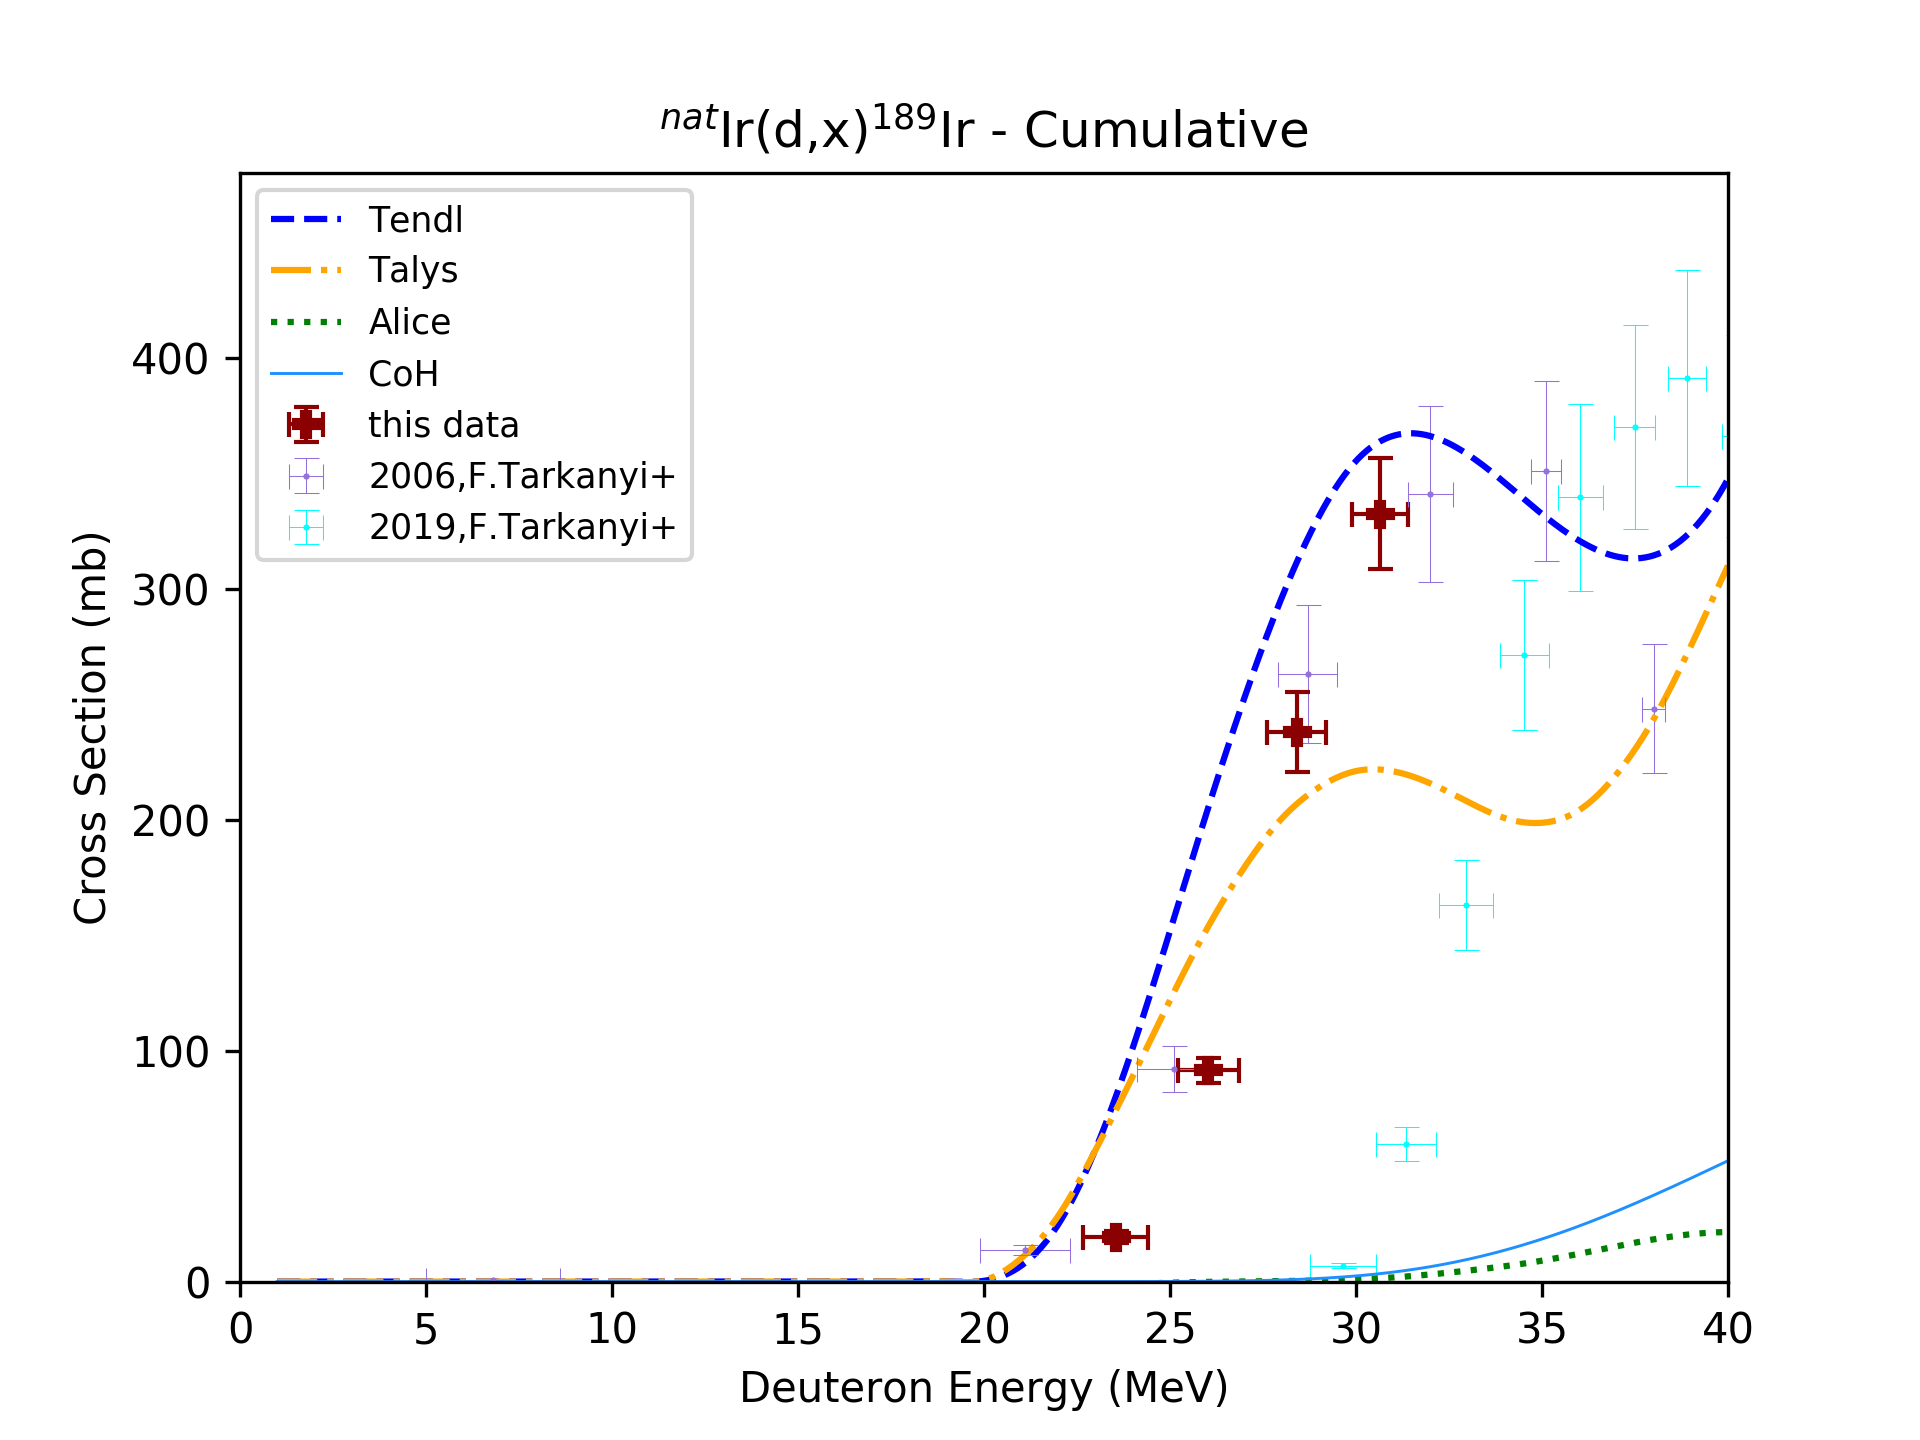
\includegraphics[width=8cm]{Results/Ir_189Ir.png} }}%
    \quad
    \subfloat[A cumulative measurement of $^{190m1+m2+g}$ (m1: 100\%, m2: 8.60\%). ]{{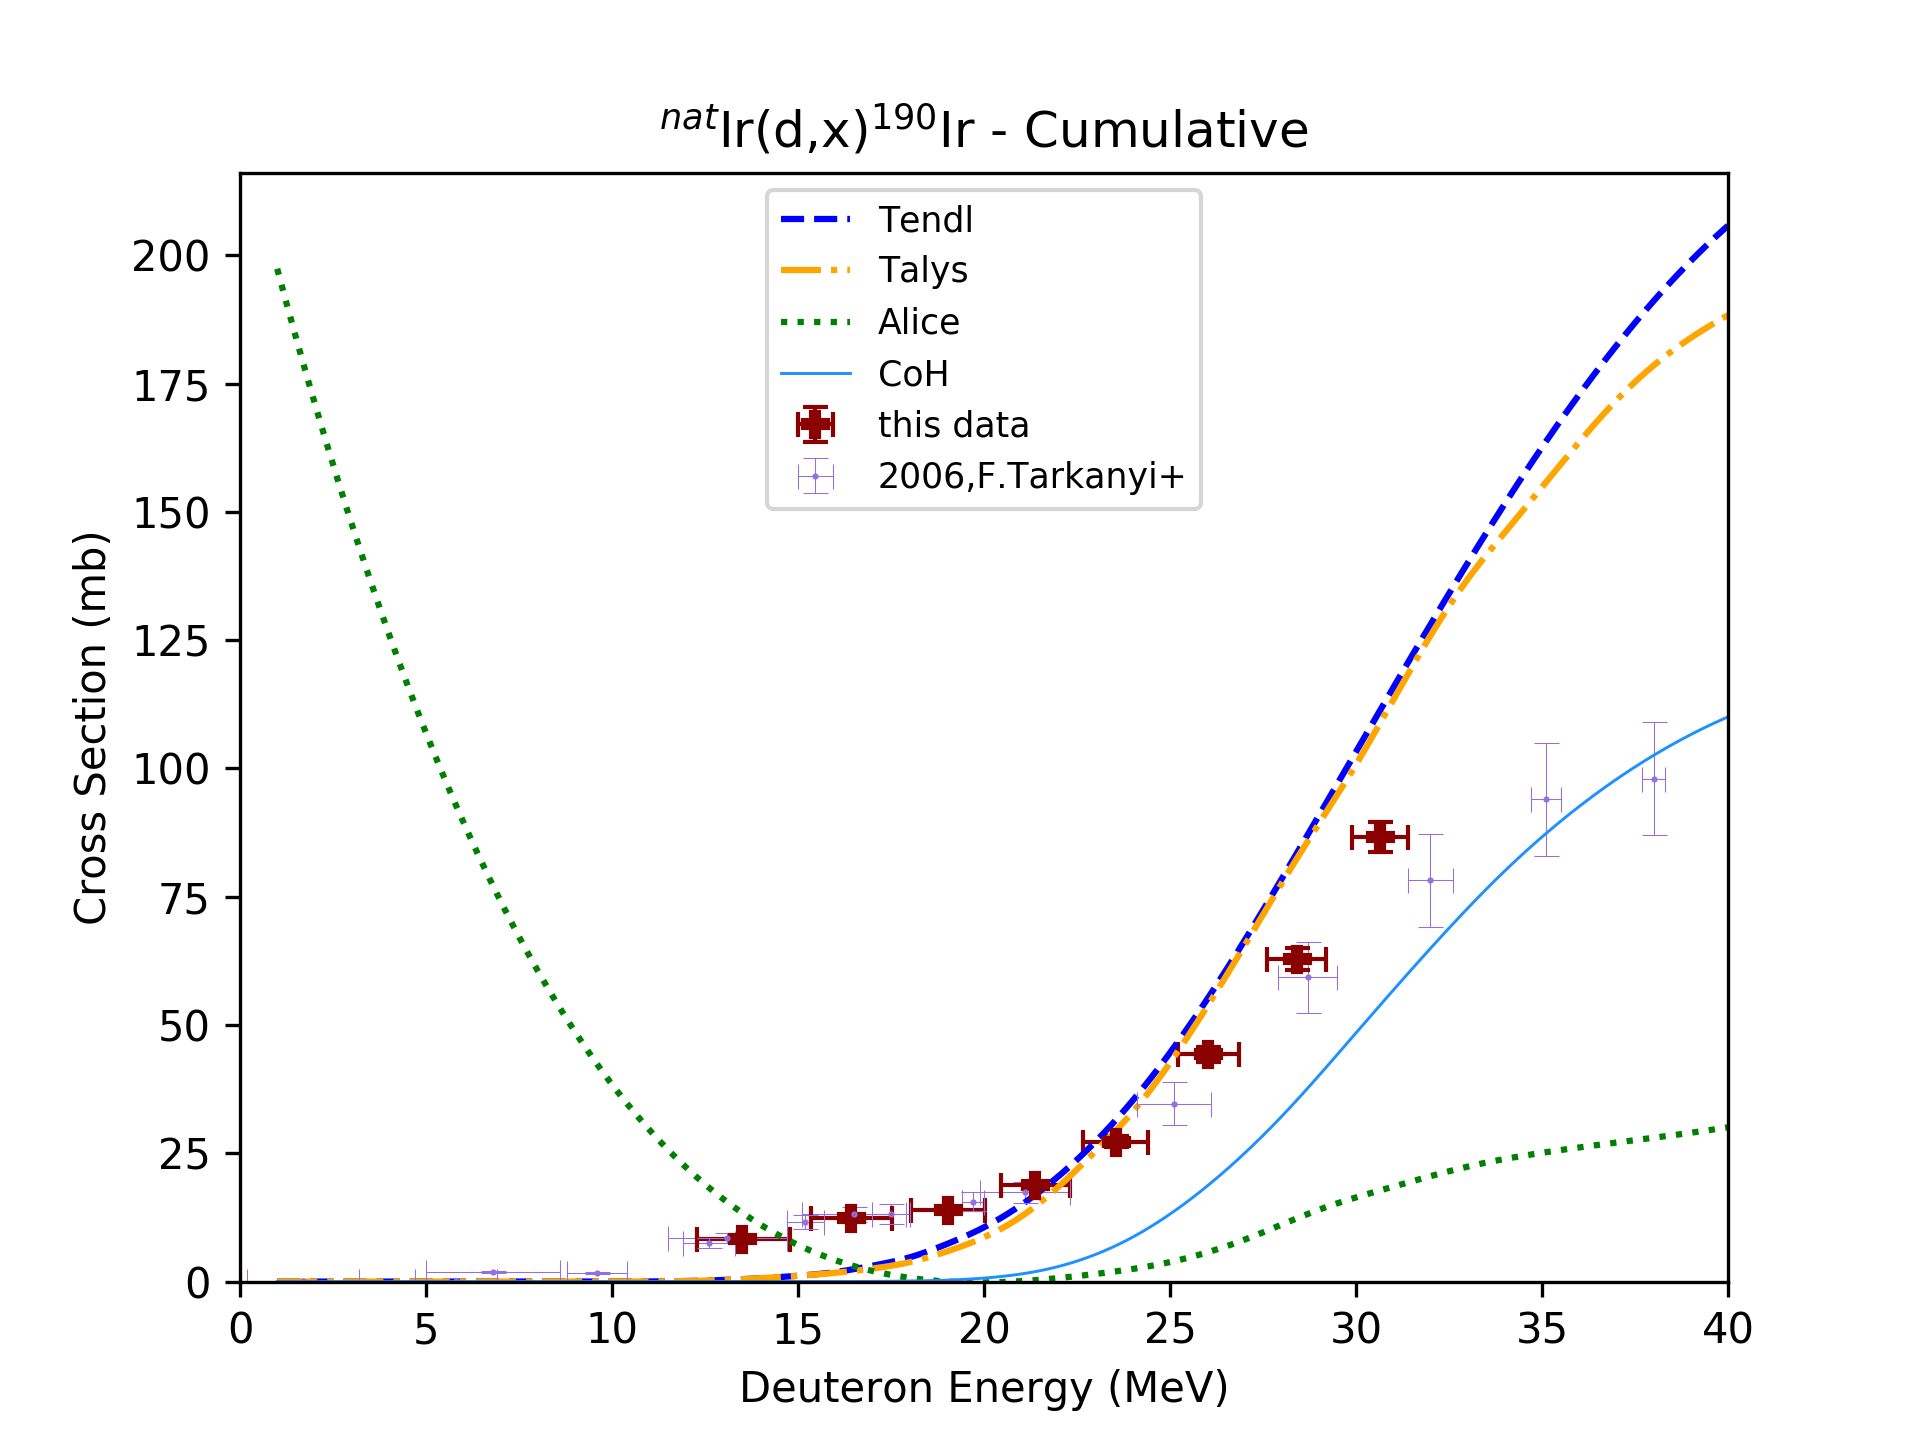
\includegraphics[width=8cm]{Results/Ir_190Ir.png} }}%
    \quad
    \subfloat[An independent measurement of the cumulative cross section for $^{190m1+g}$Ir, with subtraction of the feeding weighted percentage of $^{190m2}$Ir. ]{{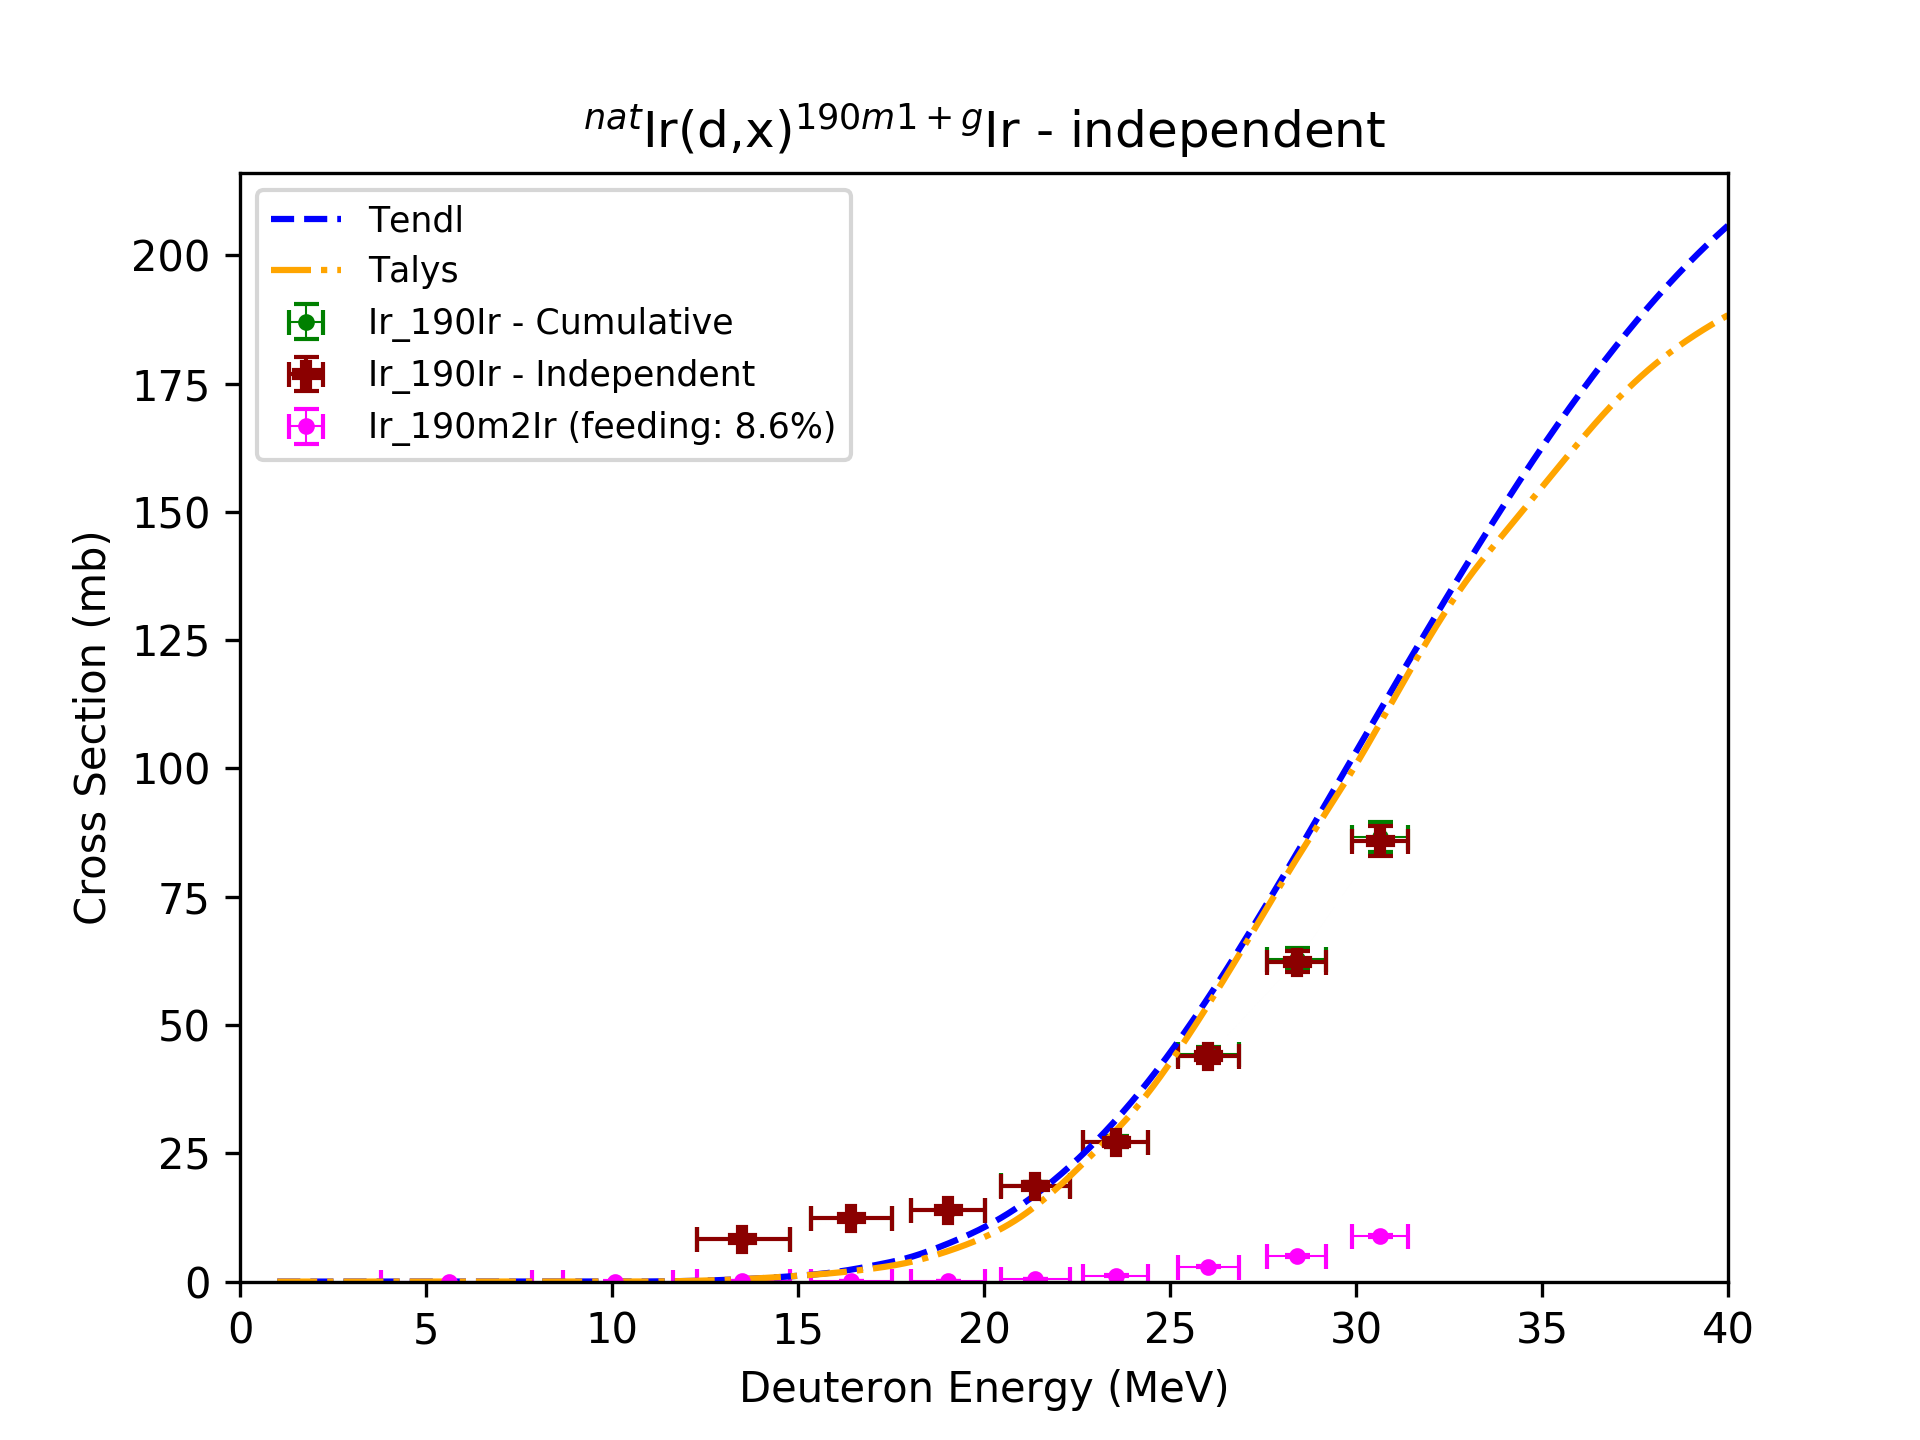
\includegraphics[width=8cm]{Results/Ir_190Ir_subtracted.png} }}%
    \quad
      \caption{Excitation functions for $^{188m1+g}$Ir (independent and cumulative) and $^{189}$Ir (cumulative)  }%
    \label{fig:cross-sections_188,189Ir}%
\end{figure}   

\begin{figure}%
    \centering
    \subfloat[An independent measurement of $^{190m2}$Ir. ]{{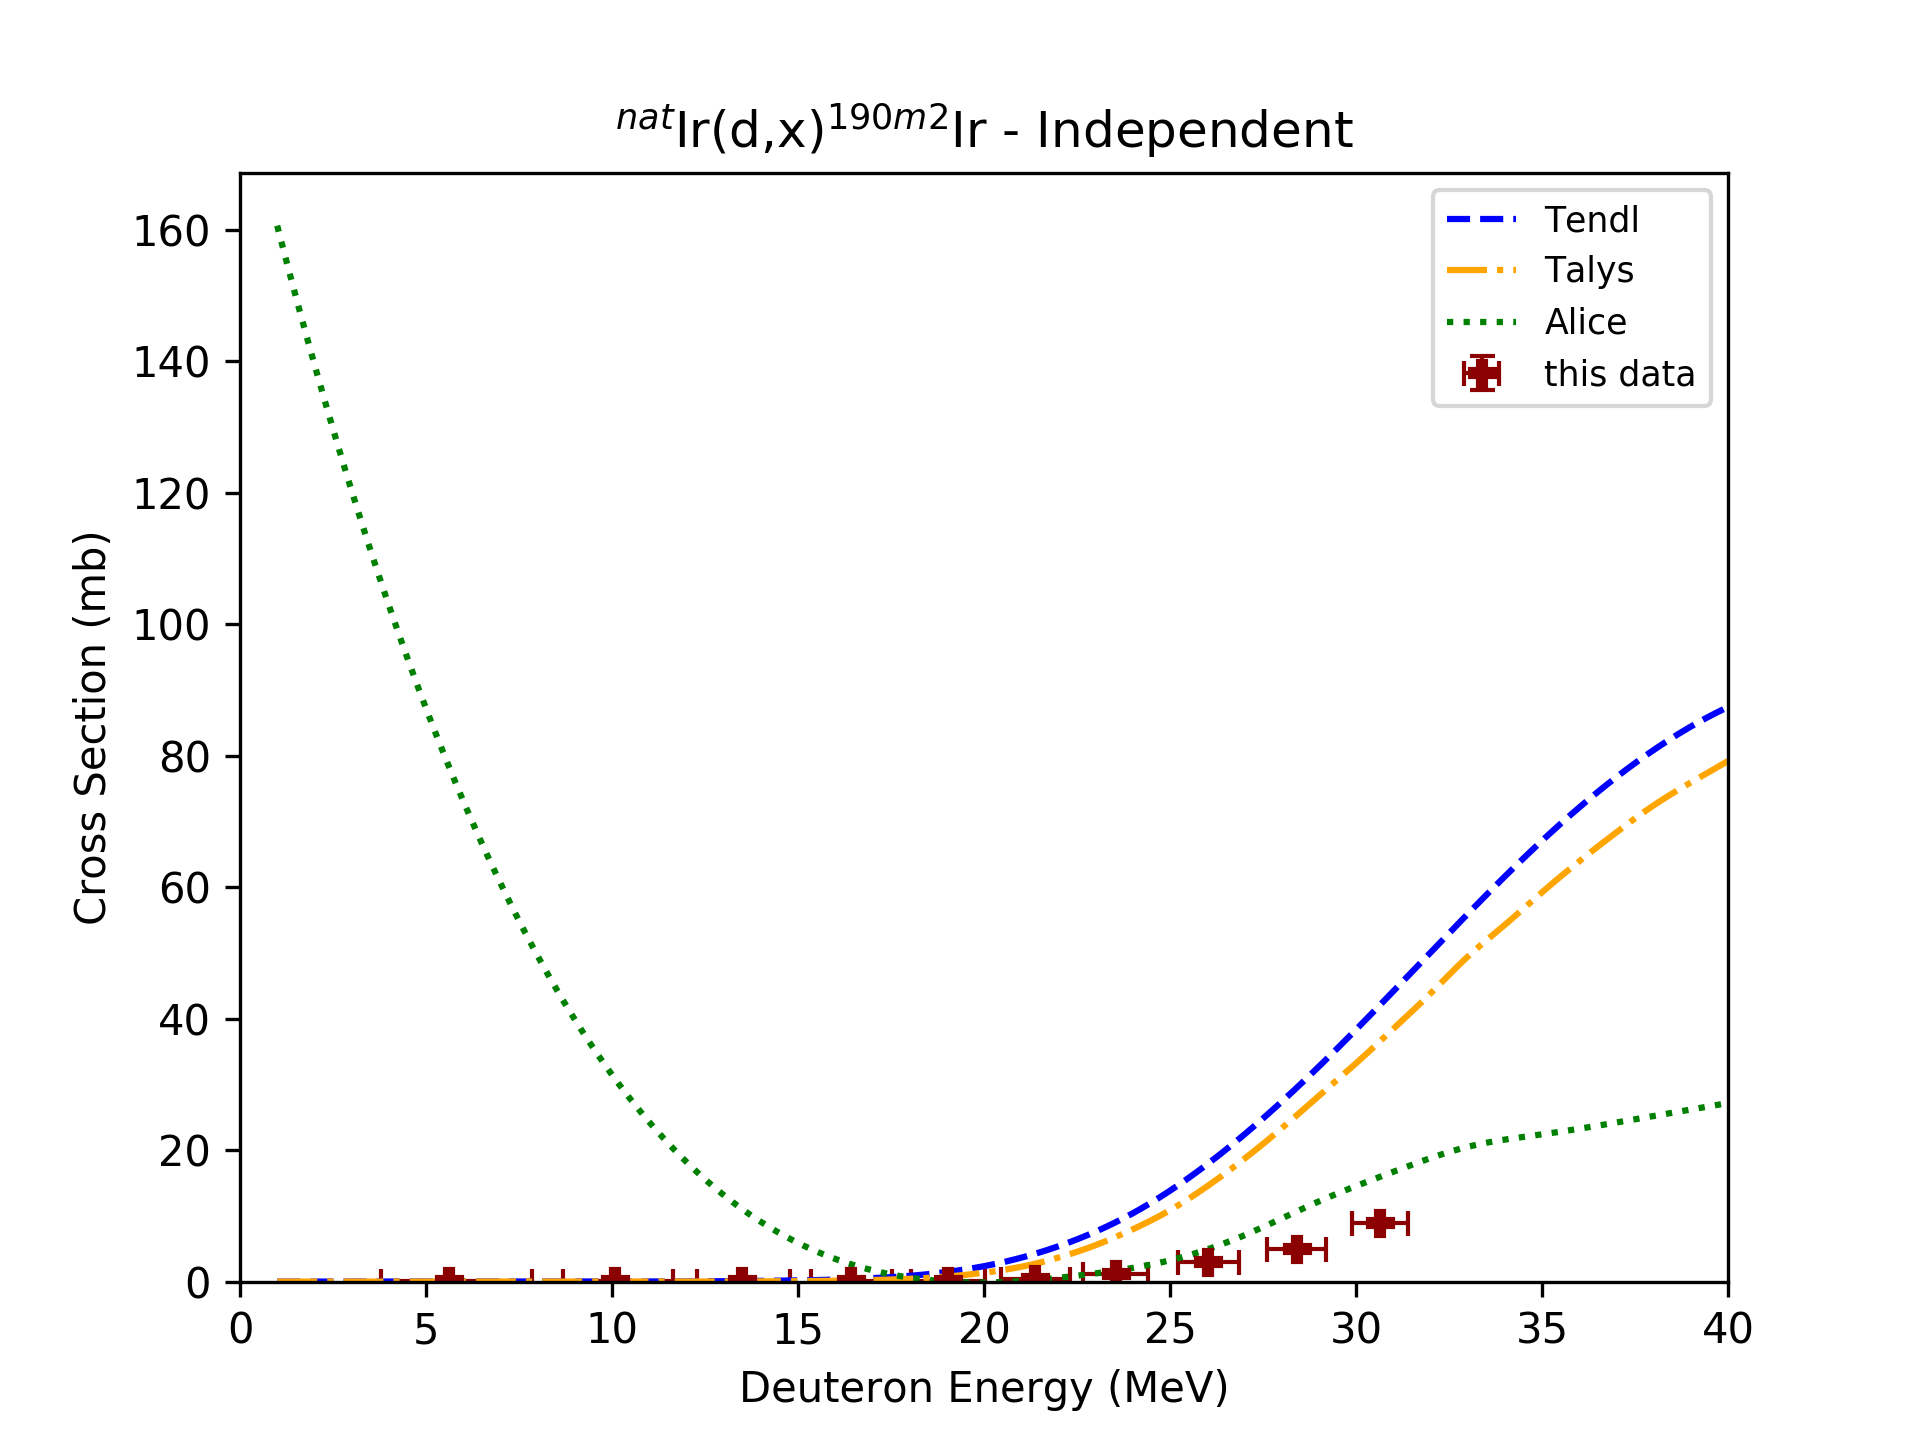
\includegraphics[width=8cm]{Results/Ir_190m2Ir.png} }}%
    \quad
    \subfloat[An independent measurement of the cumulative cross section for $^{192}$Ir isomers (m1: 99.98\%, m2: 100\%)]{{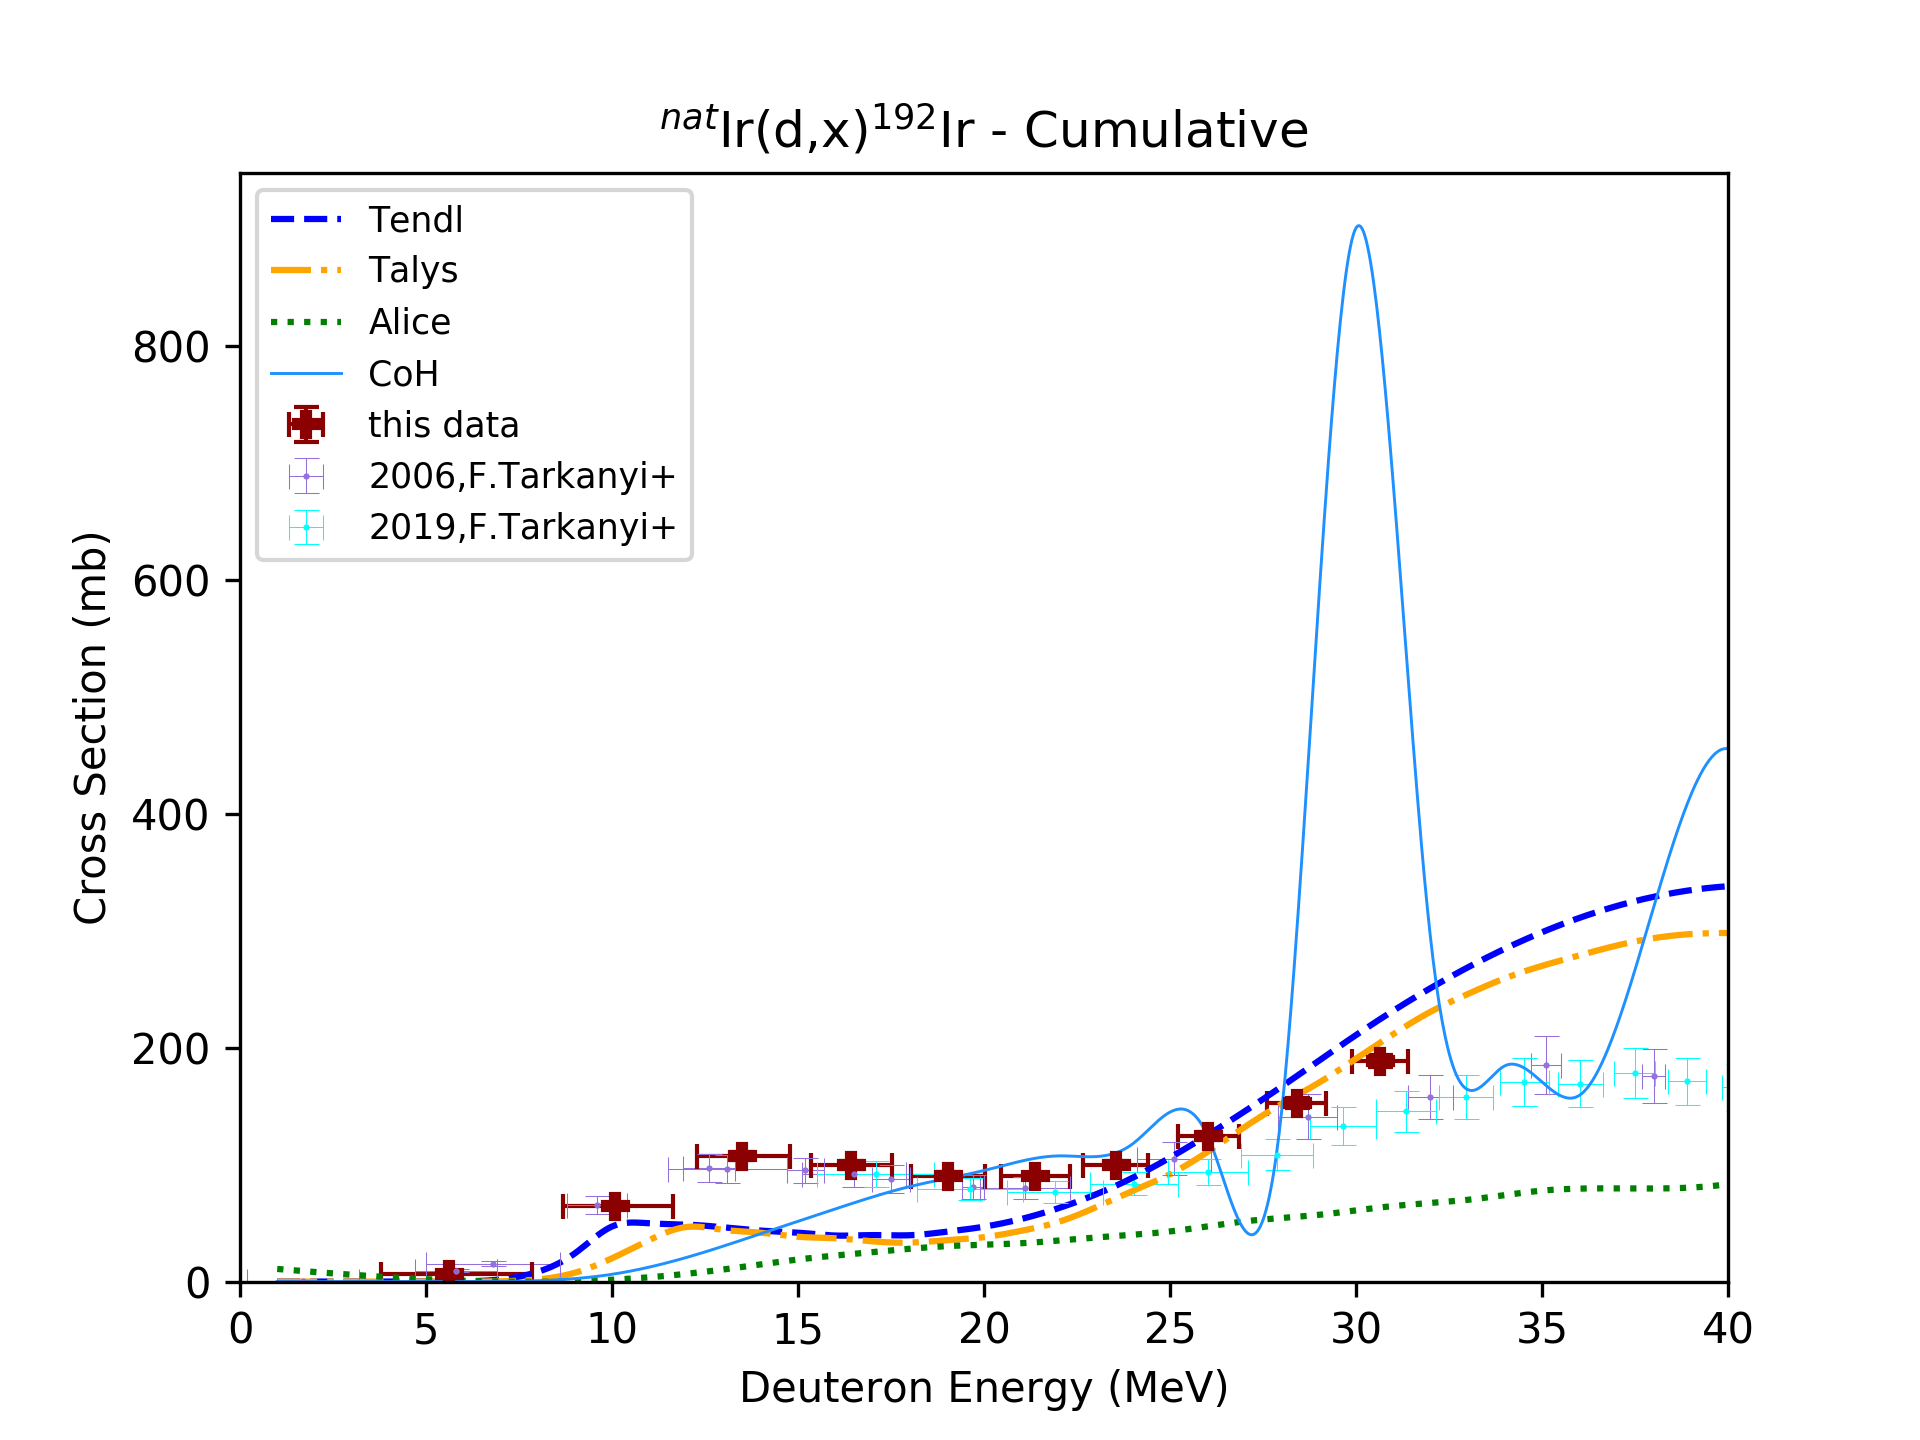
\includegraphics[width=8cm]{Results/Ir_192Ir.png} }}%
    \quad
    \subfloat[An independent measurement of the cumulative cross section for $^{194m1+g}$ (m1:100\%)]{{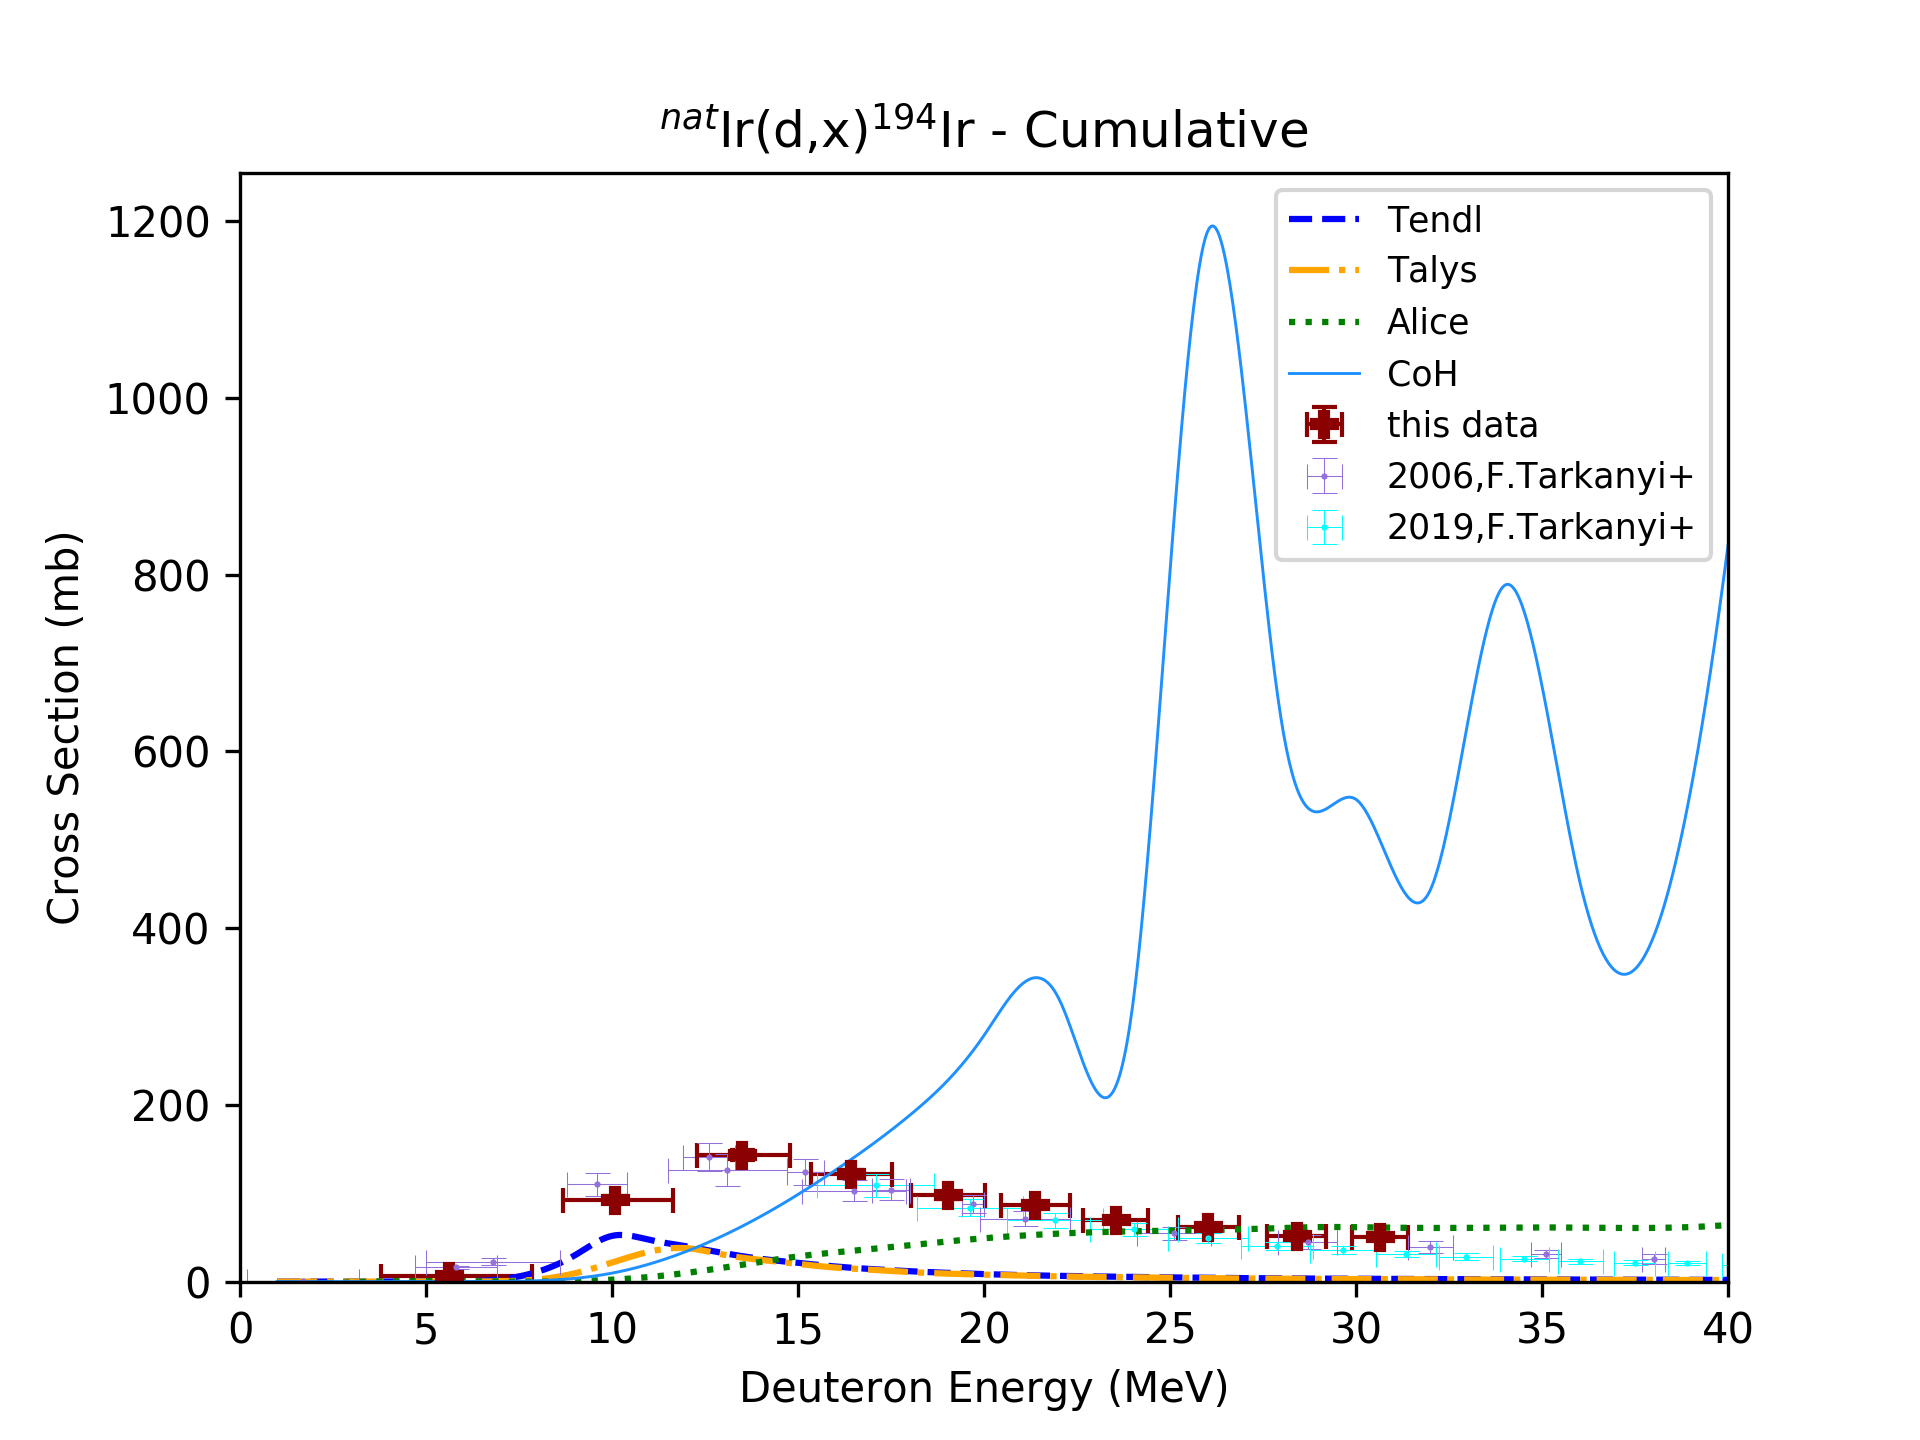
\includegraphics[width=8cm]{Results/Ir_194Ir.png} }}%
    \quad
    \subfloat[An independent measurement of $^{194m2}$Ir. ]{{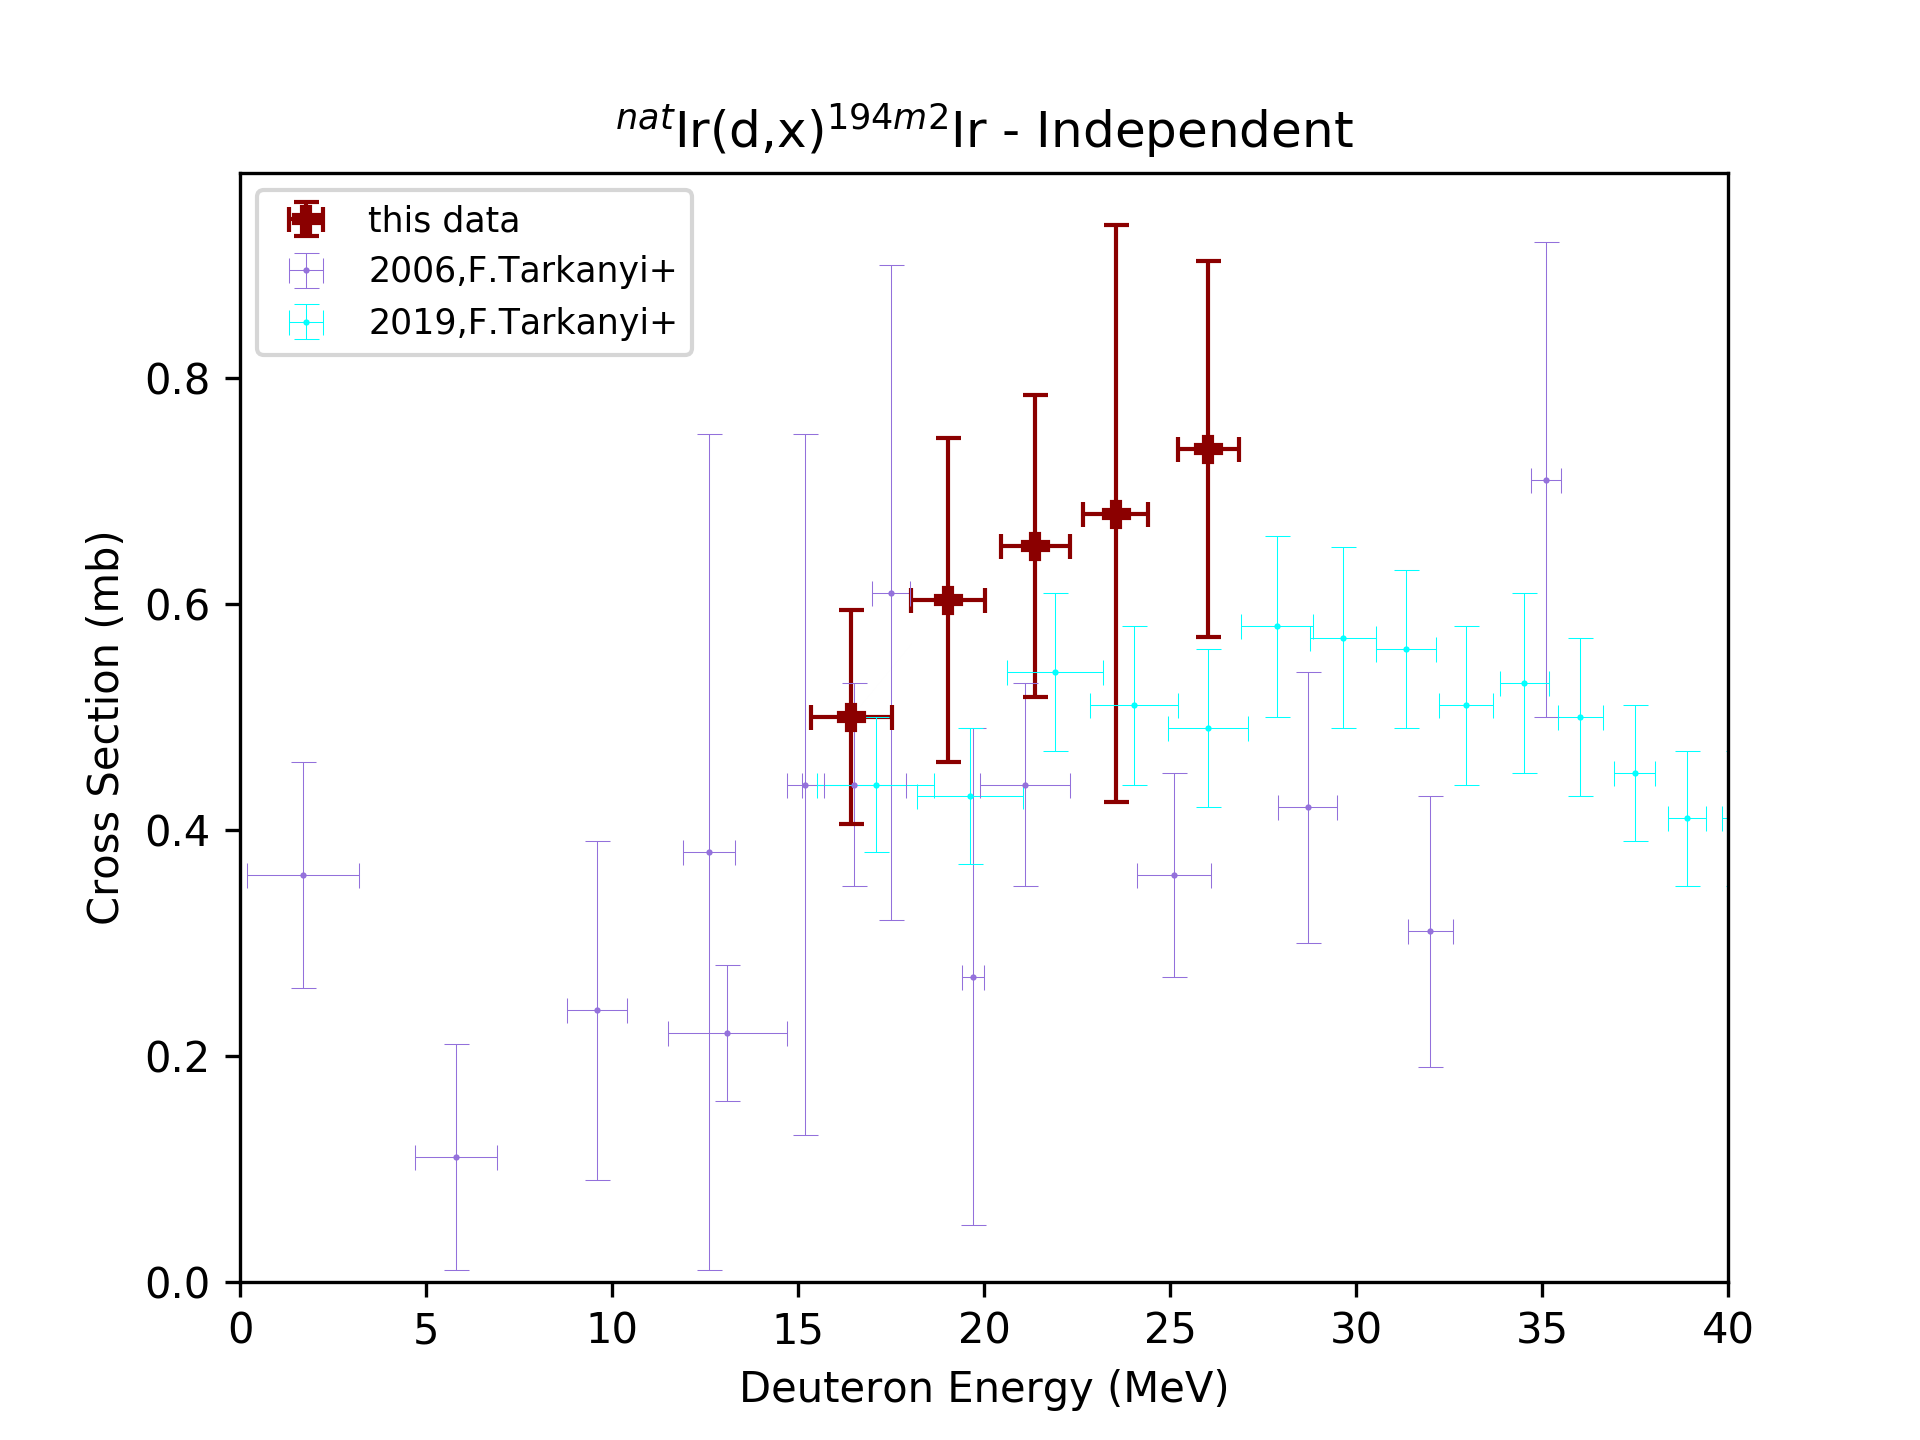
\includegraphics[width=8cm]{Results/Ir_194m2Ir.png} }}%
    \caption{Excitation functions for $^{190m1+m2+g}$Ir (cumulative), $^{190m1+g}$Ir (cumulative), $^{190m2}$Ir (independent), $^{194m1+g}$Ir (cumulative) and $^{194m2}$Ir (independent)  }%
    \label{fig:cross-sections_190,194Ir}%
\end{figure}







\begin{figure}%
    \centering
    \subfloat[An independent measurement of $^{188}$Pt. ]{{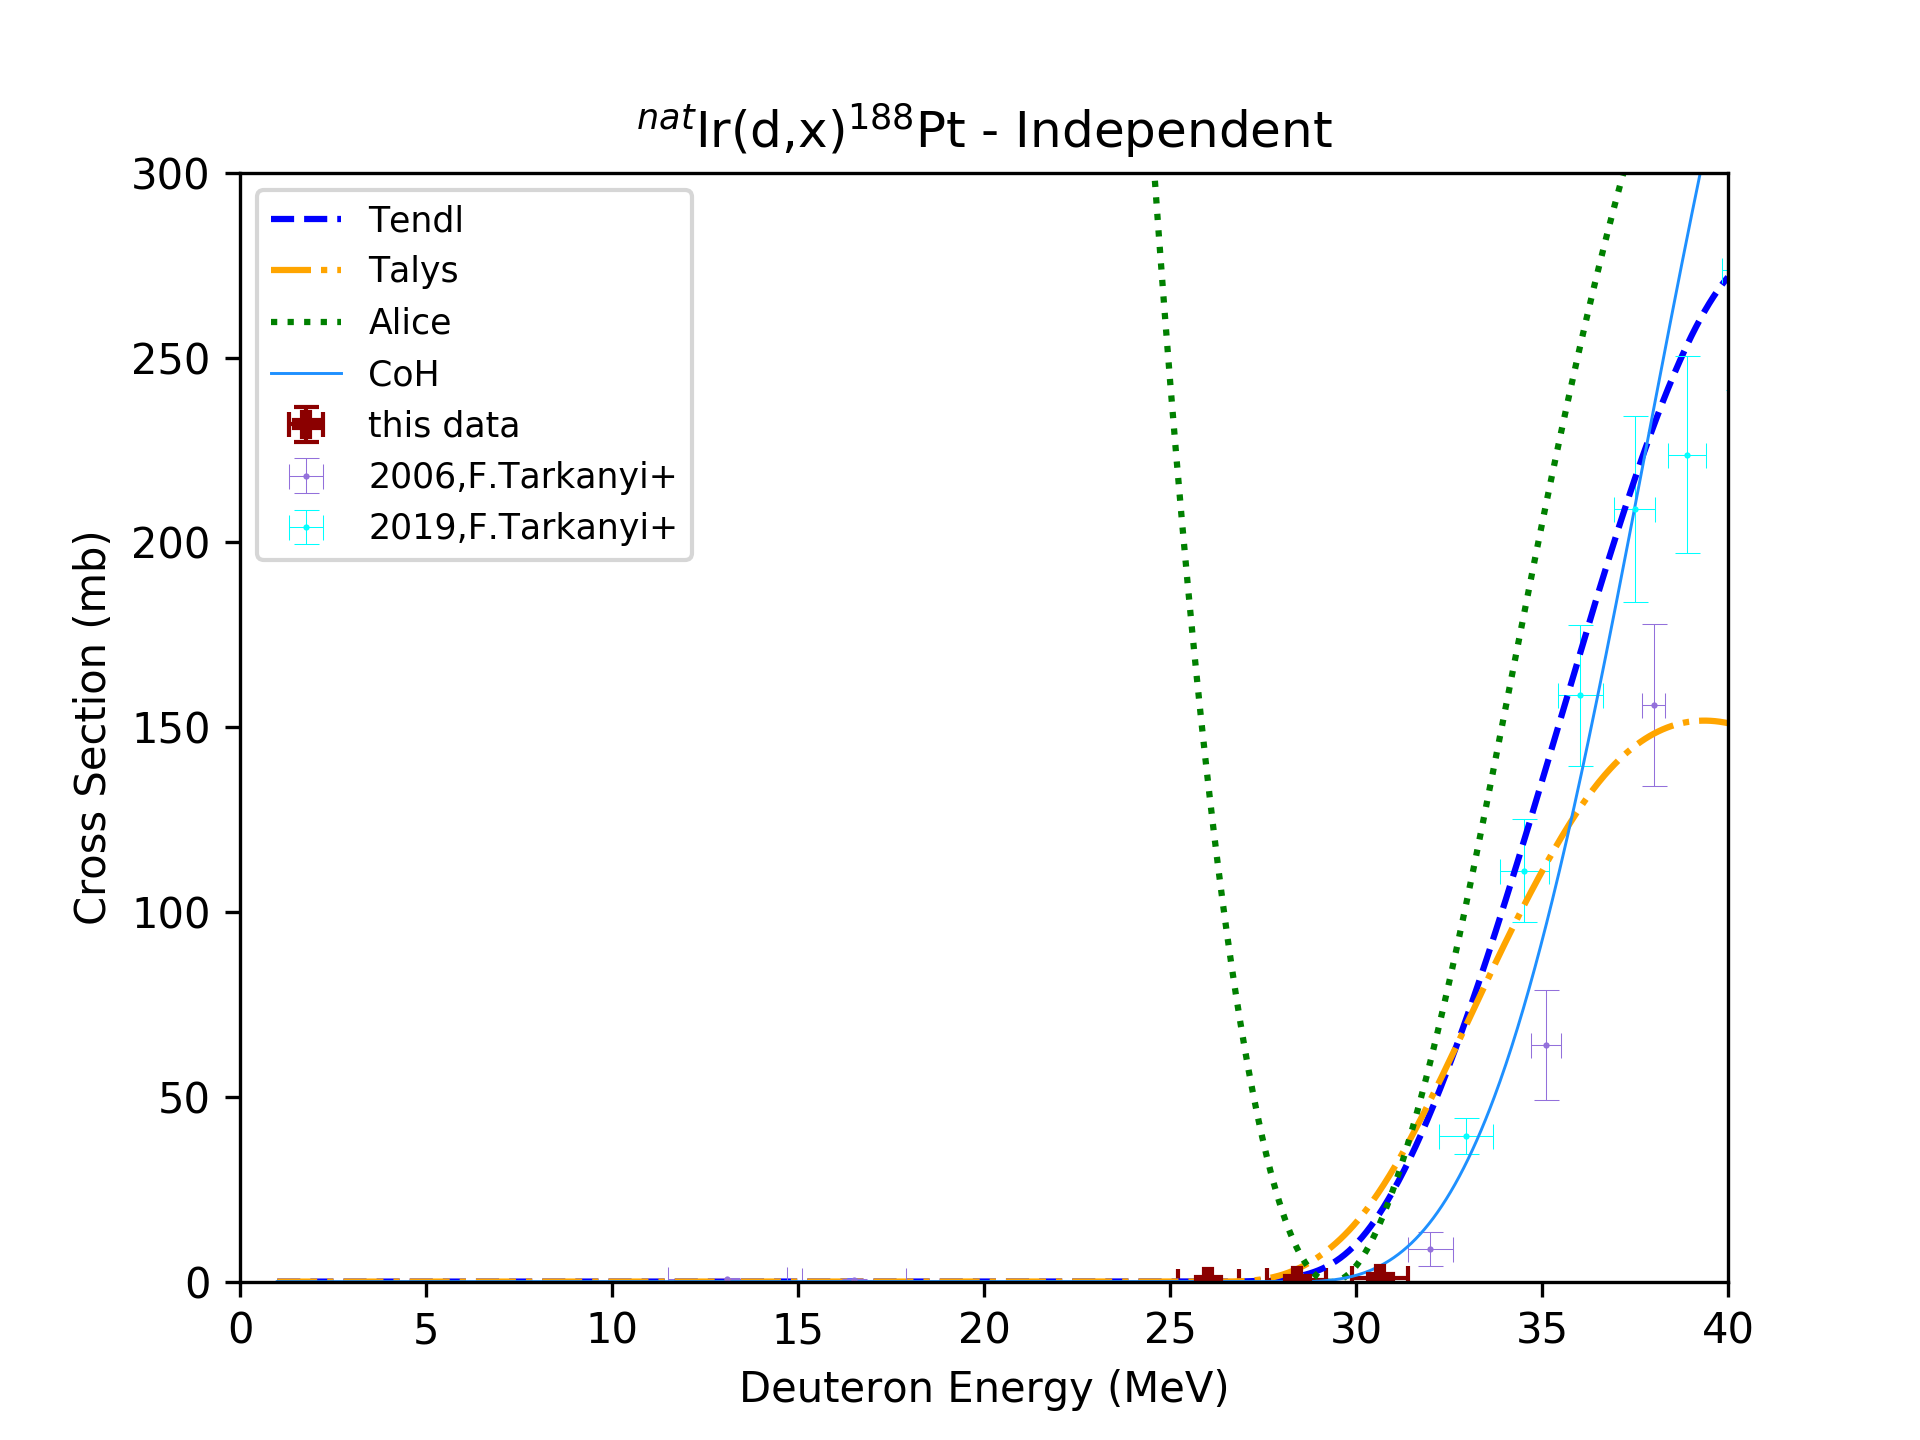
\includegraphics[width=8cm]{Results/Ir_188Pt.png} }}%
    \quad
    \subfloat[An independent measurement of $^{189}$Pt. ]{{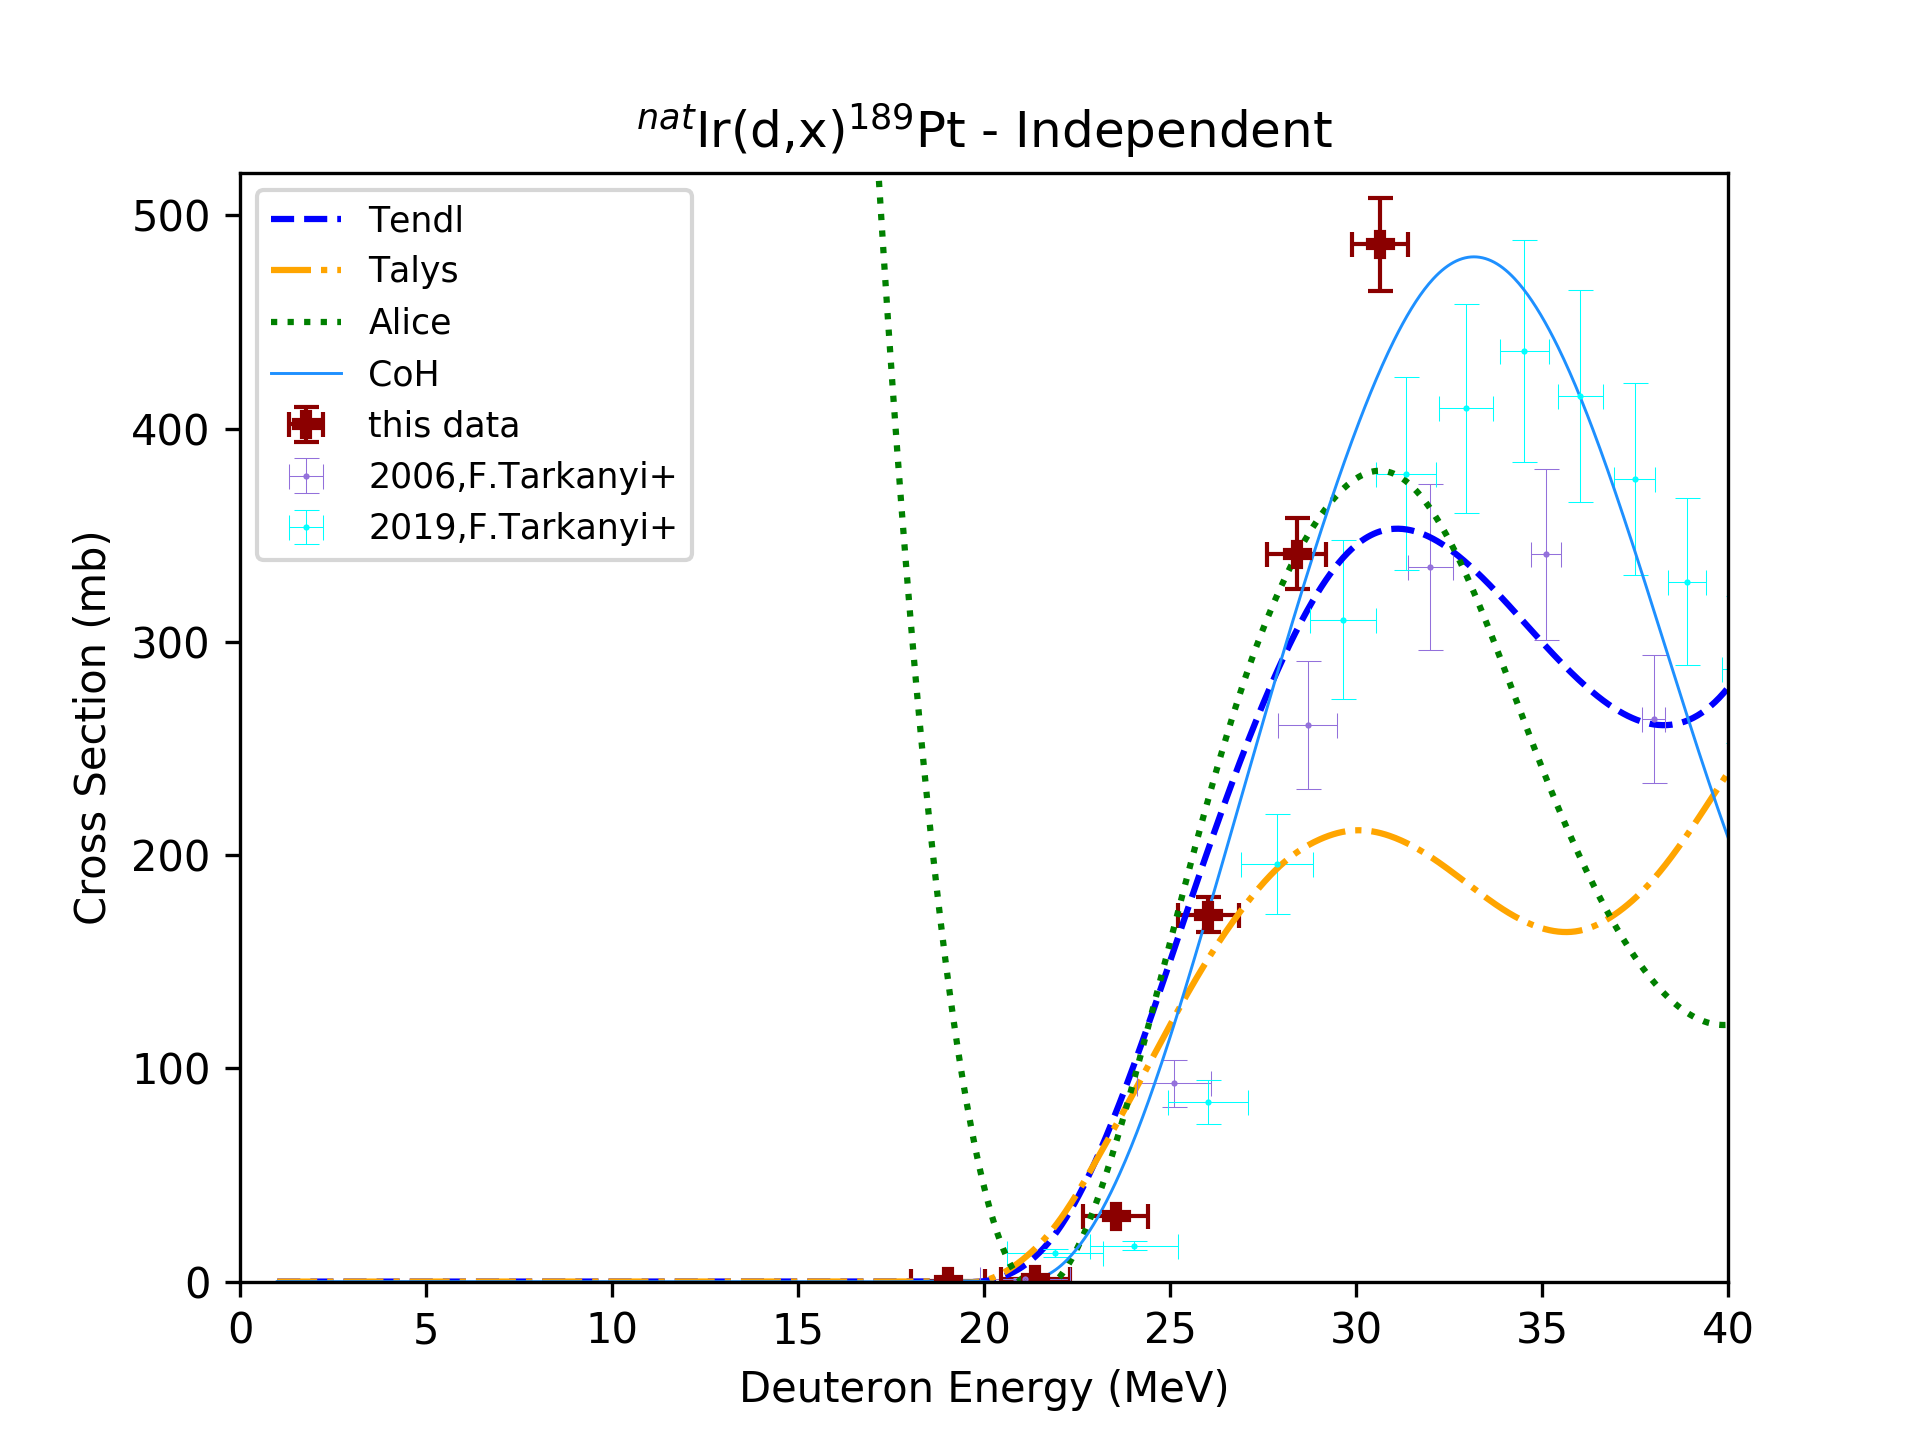
\includegraphics[width=8cm]{Results/Ir_189Pt.png} }}%
    \quad
    \subfloat[An independent measurement of $^{191}$Pt. ]{{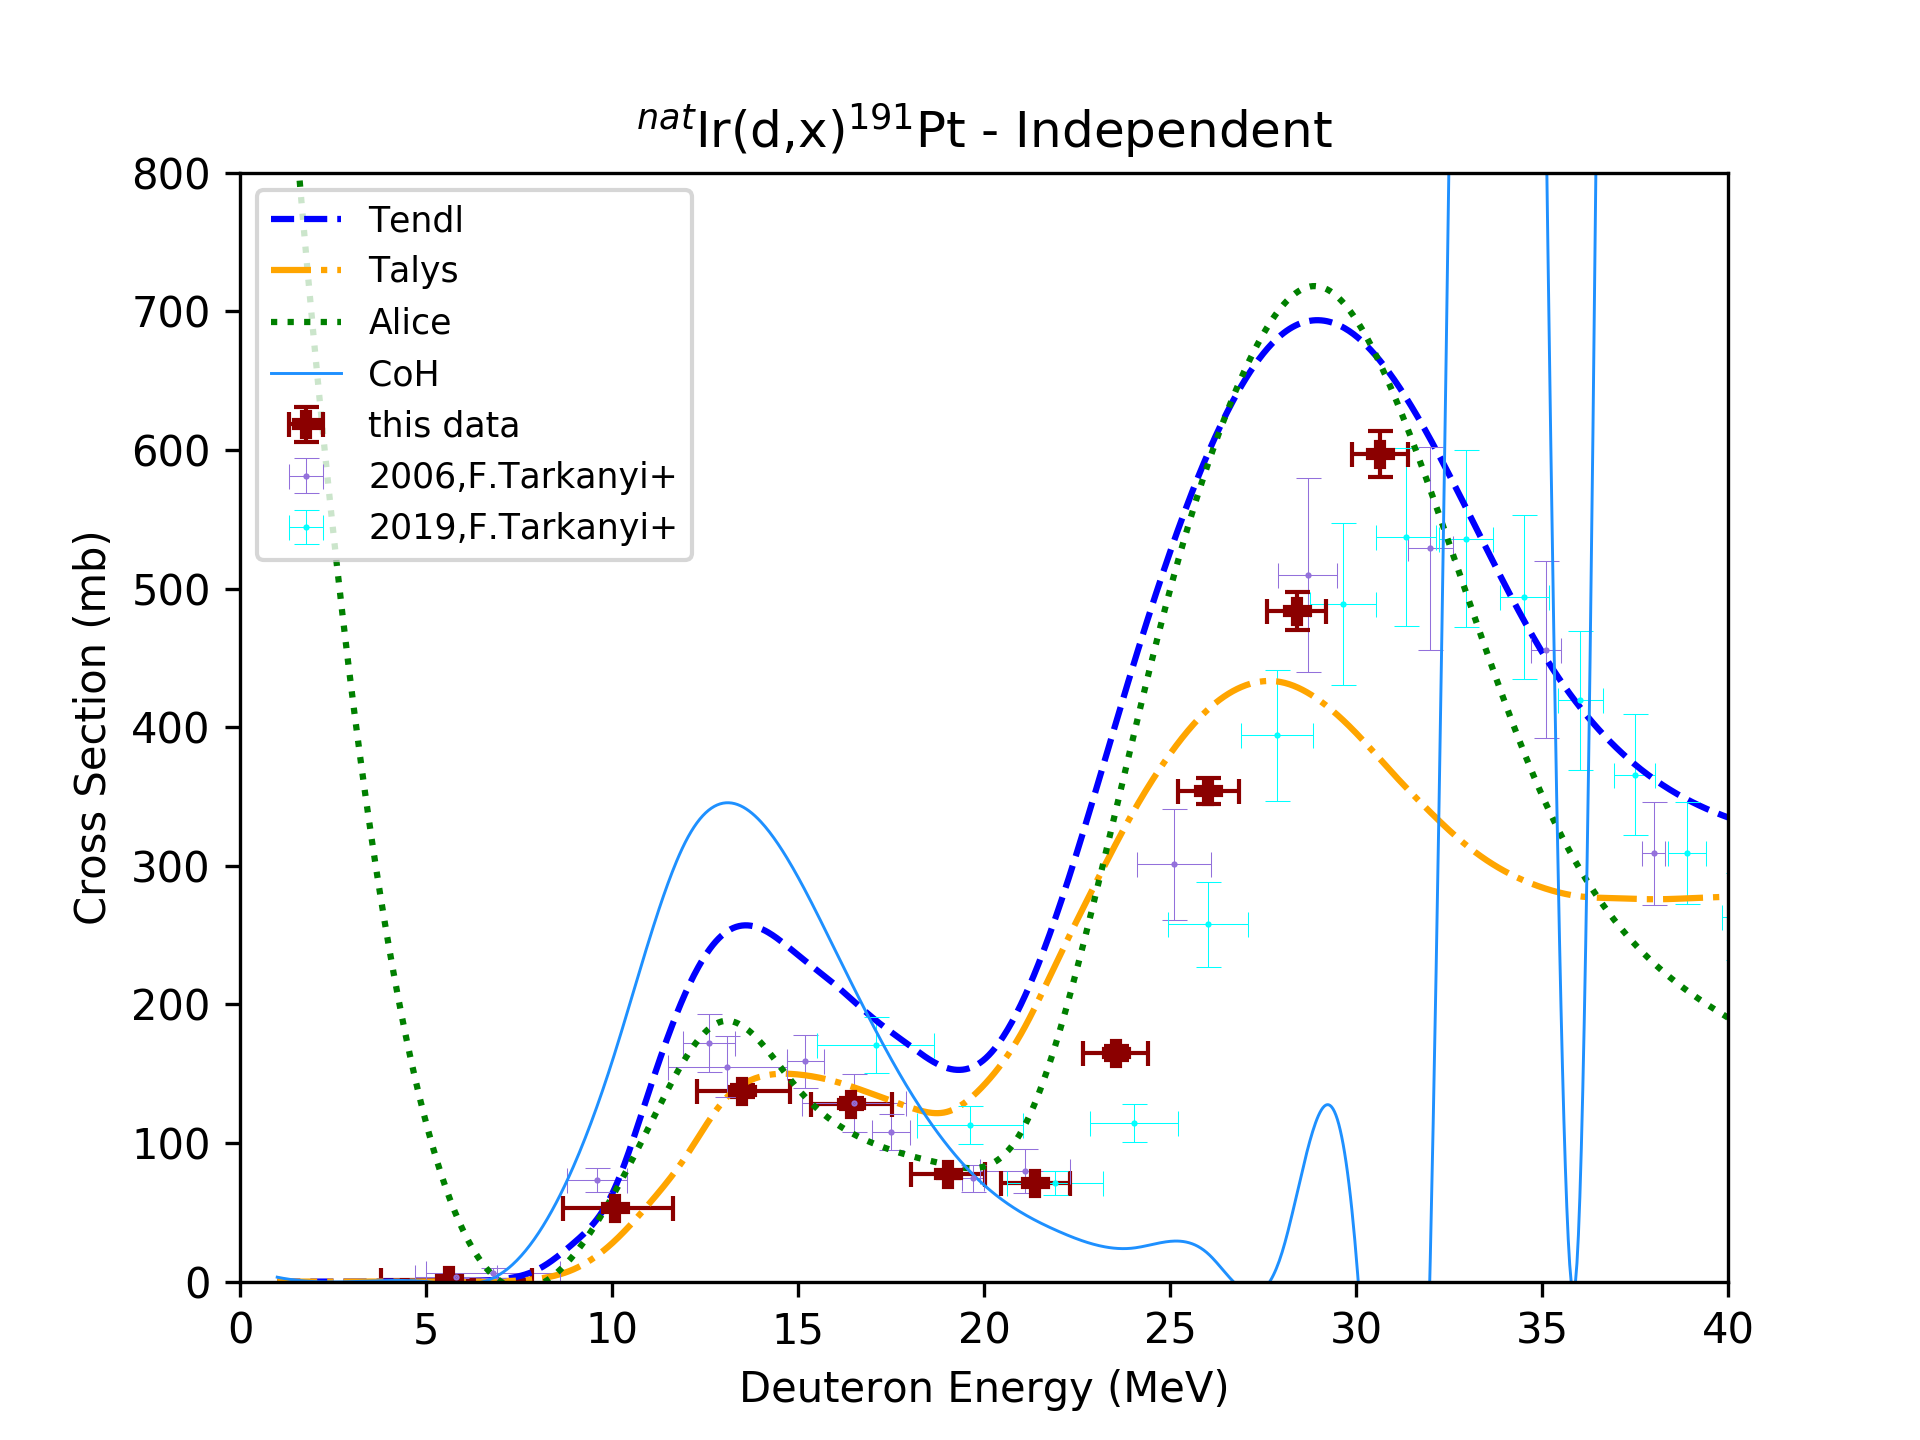
\includegraphics[width=8cm]{Results/Ir_191Pt.png} }}%
    \quad
    \subfloat[An independent measurement of $^{193m}$Pt.]{{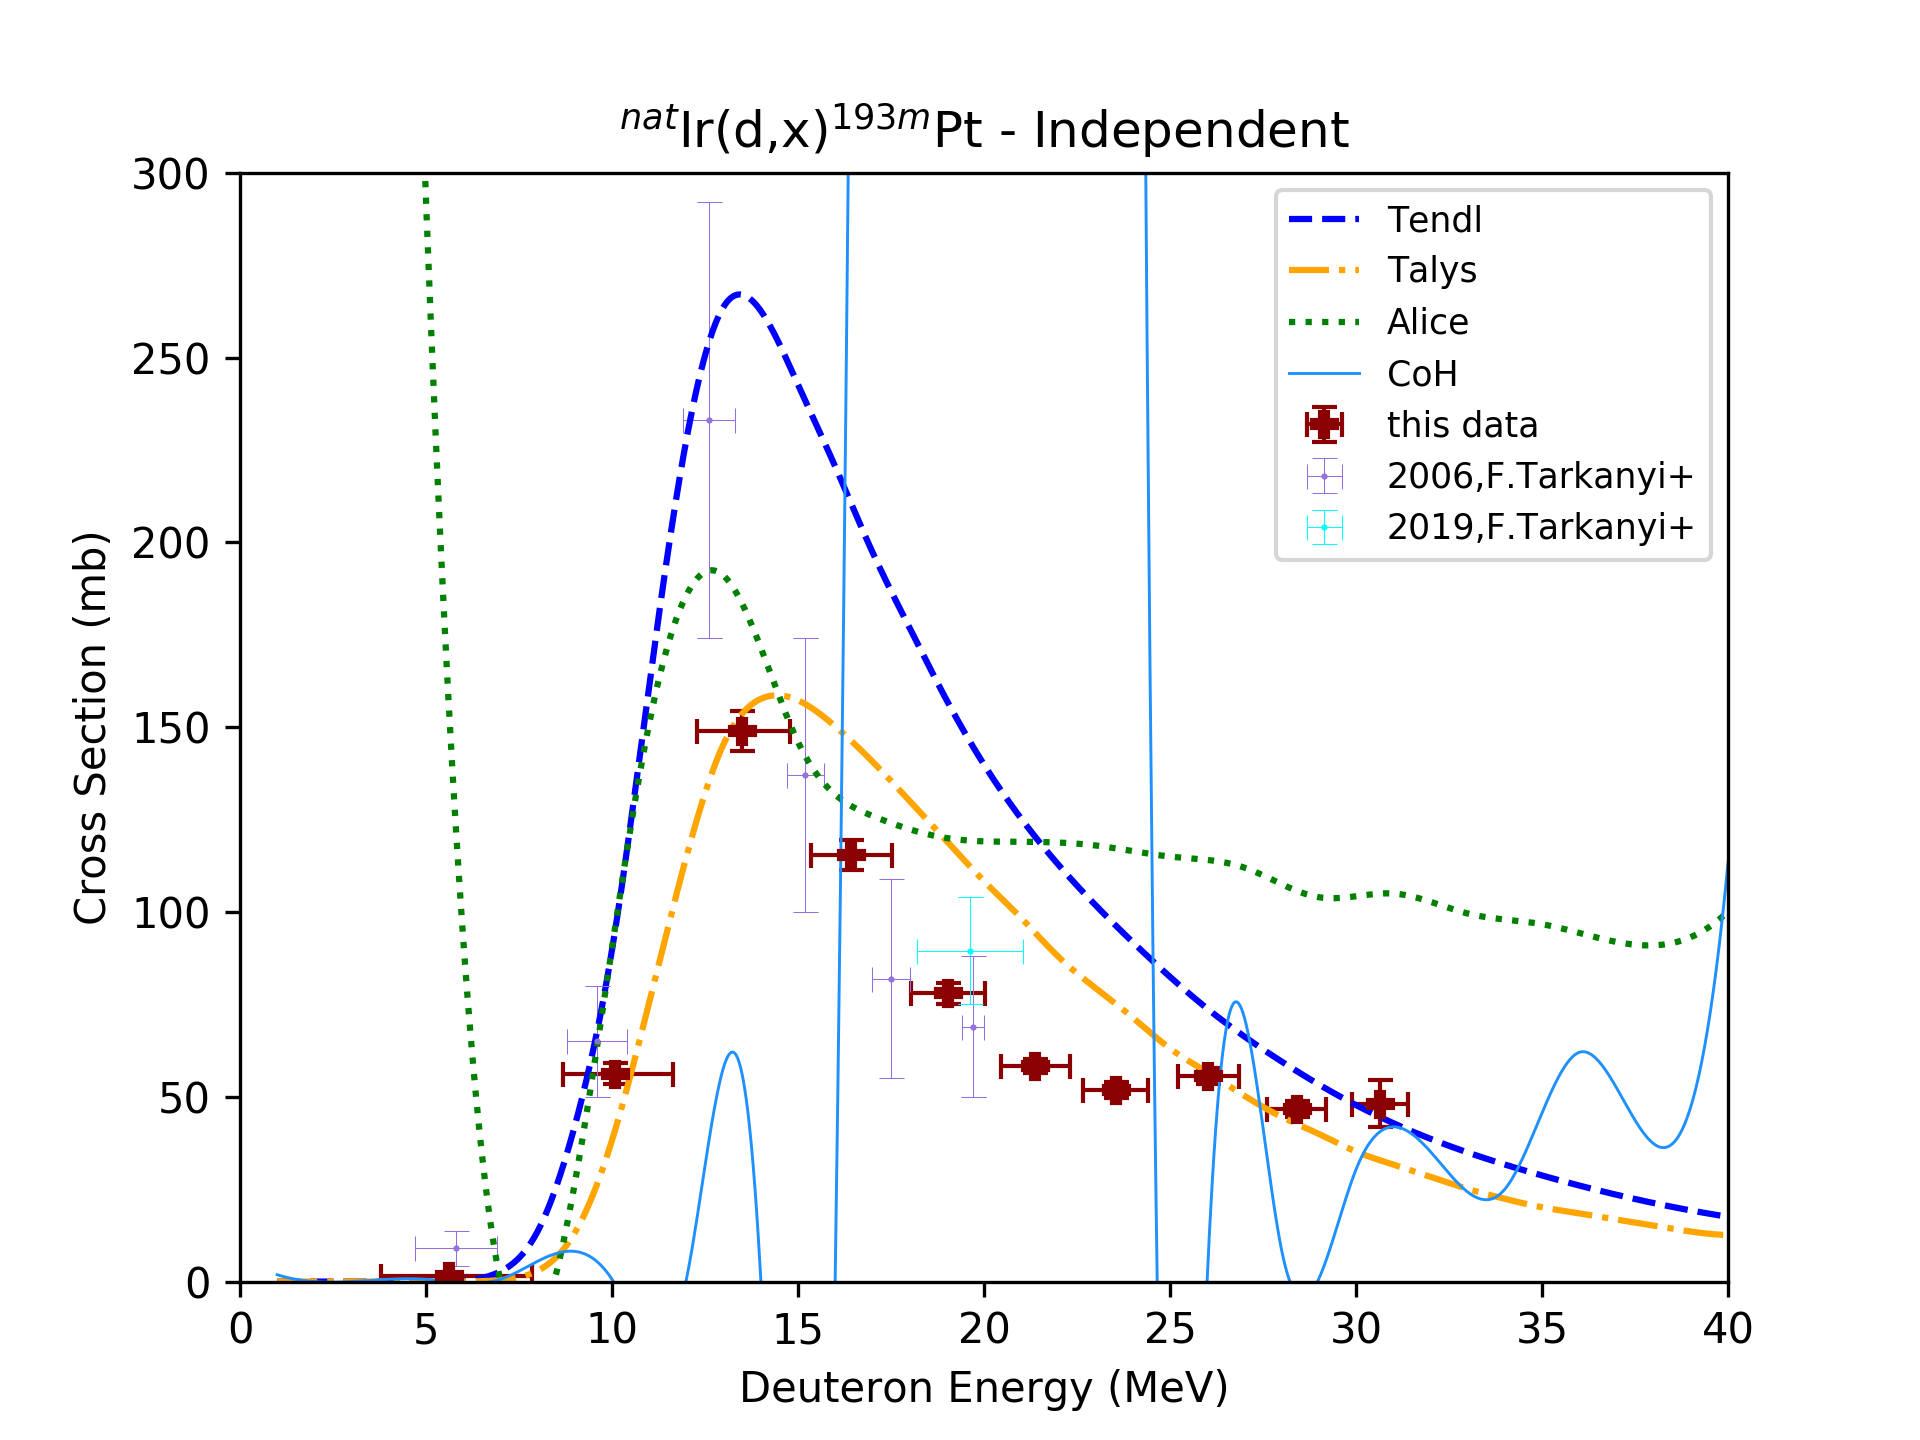
\includegraphics[width=8cm]{Results/Ir_193mPt.png} }}%
    \quad 
    \caption{Excitation functions for Platinum radionuclides }%
    \label{fig:cross-sections_Pt}%
\end{figure}

\begin{figure}%
    \centering
    \subfloat[A cumulative measurement of $^{48}$V. ]{{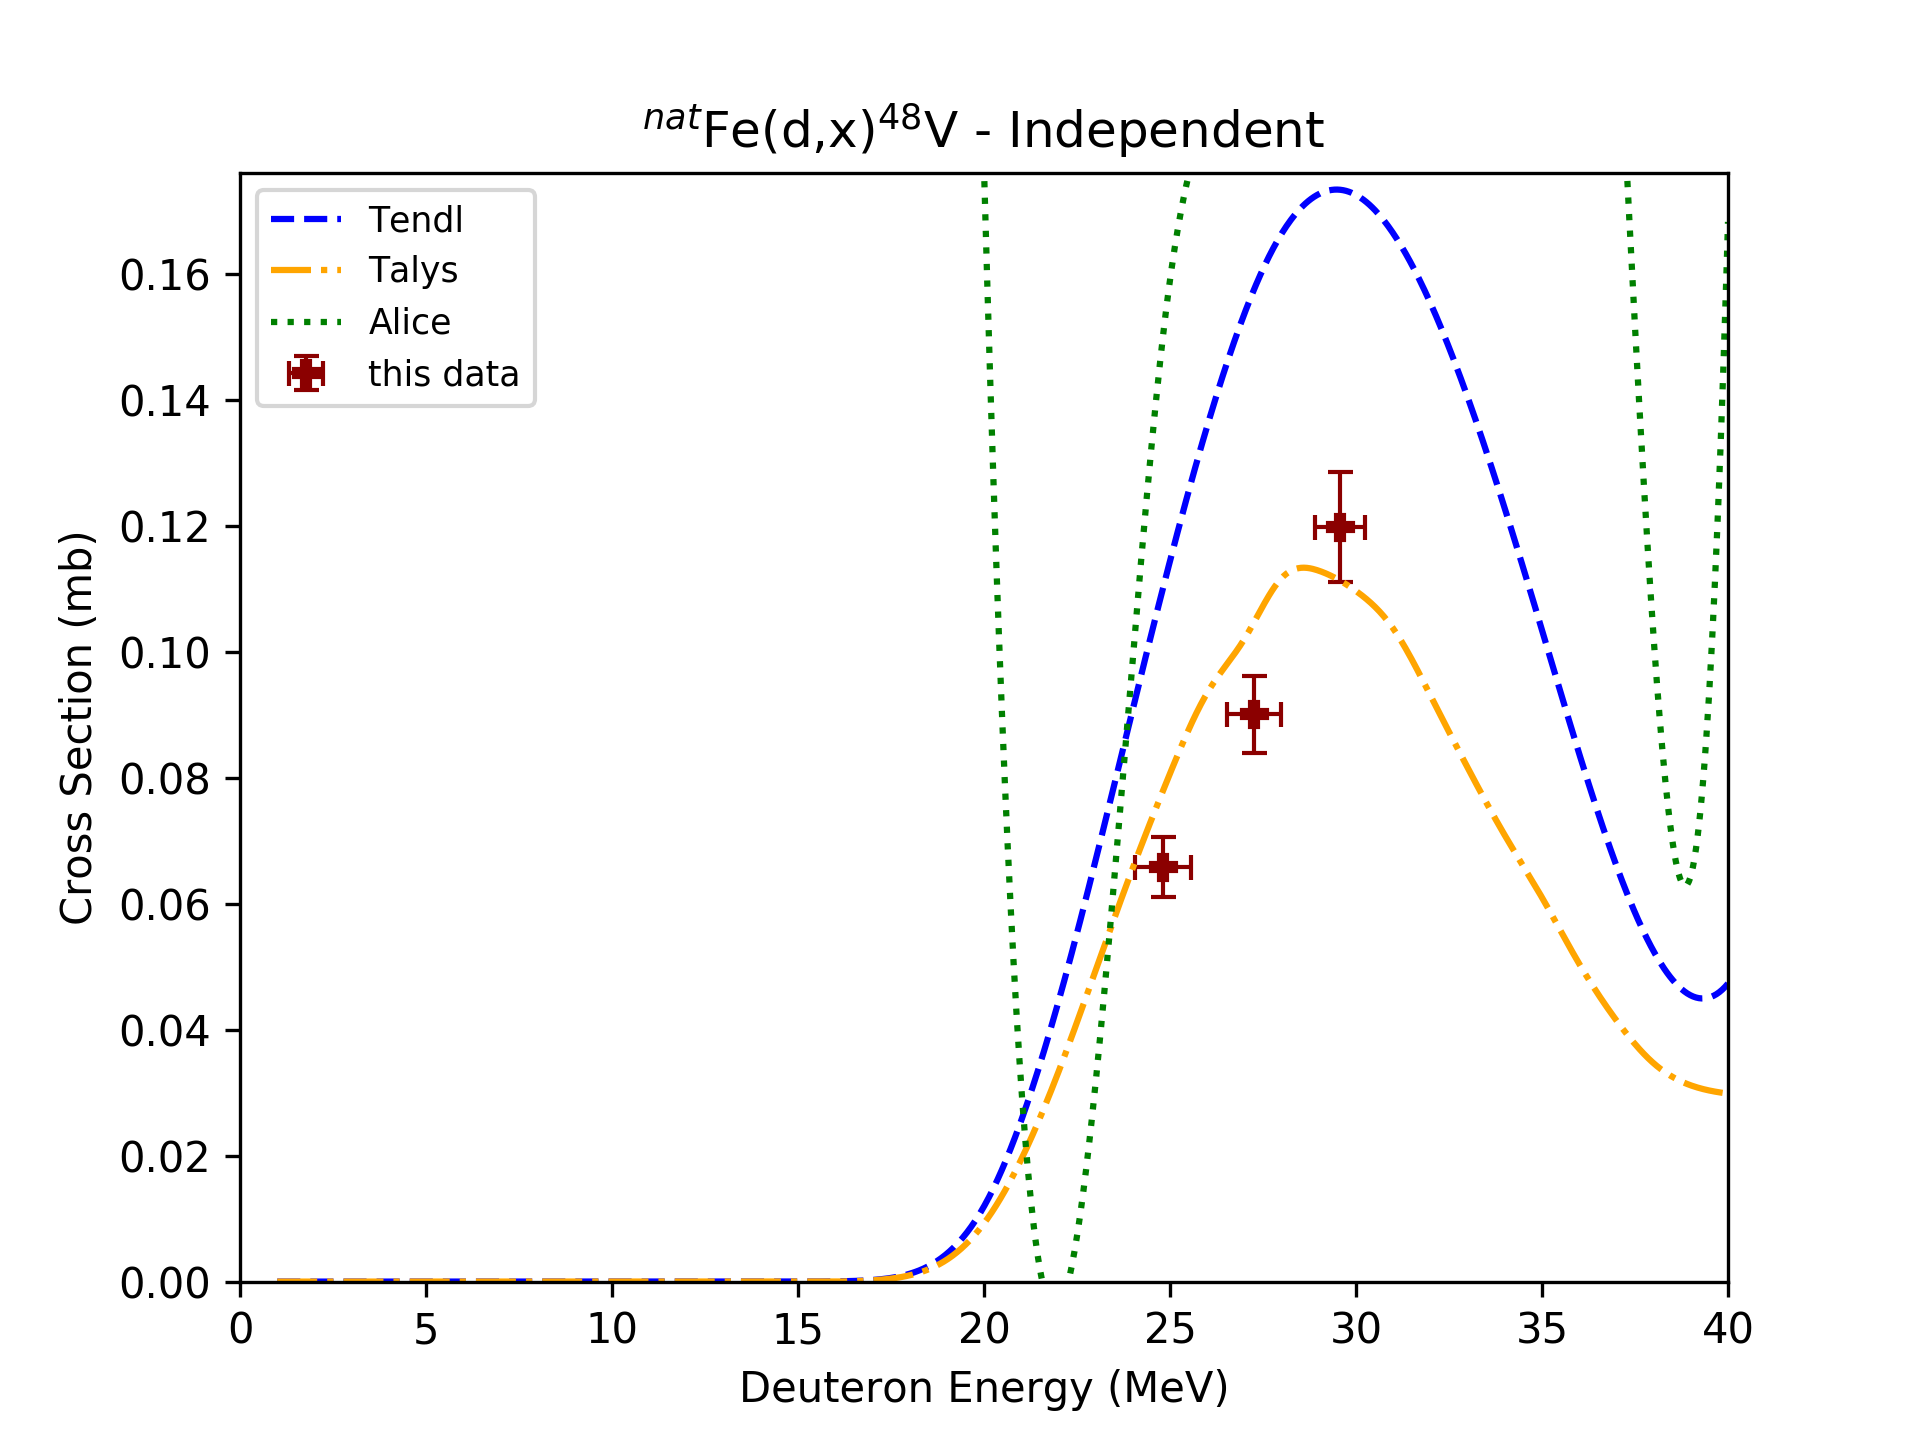
\includegraphics[width=8cm]{Results/Fe_48V.png} }}%
    \quad
    \subfloat[A cumulative measurement of $^{51}$Cr. ]{{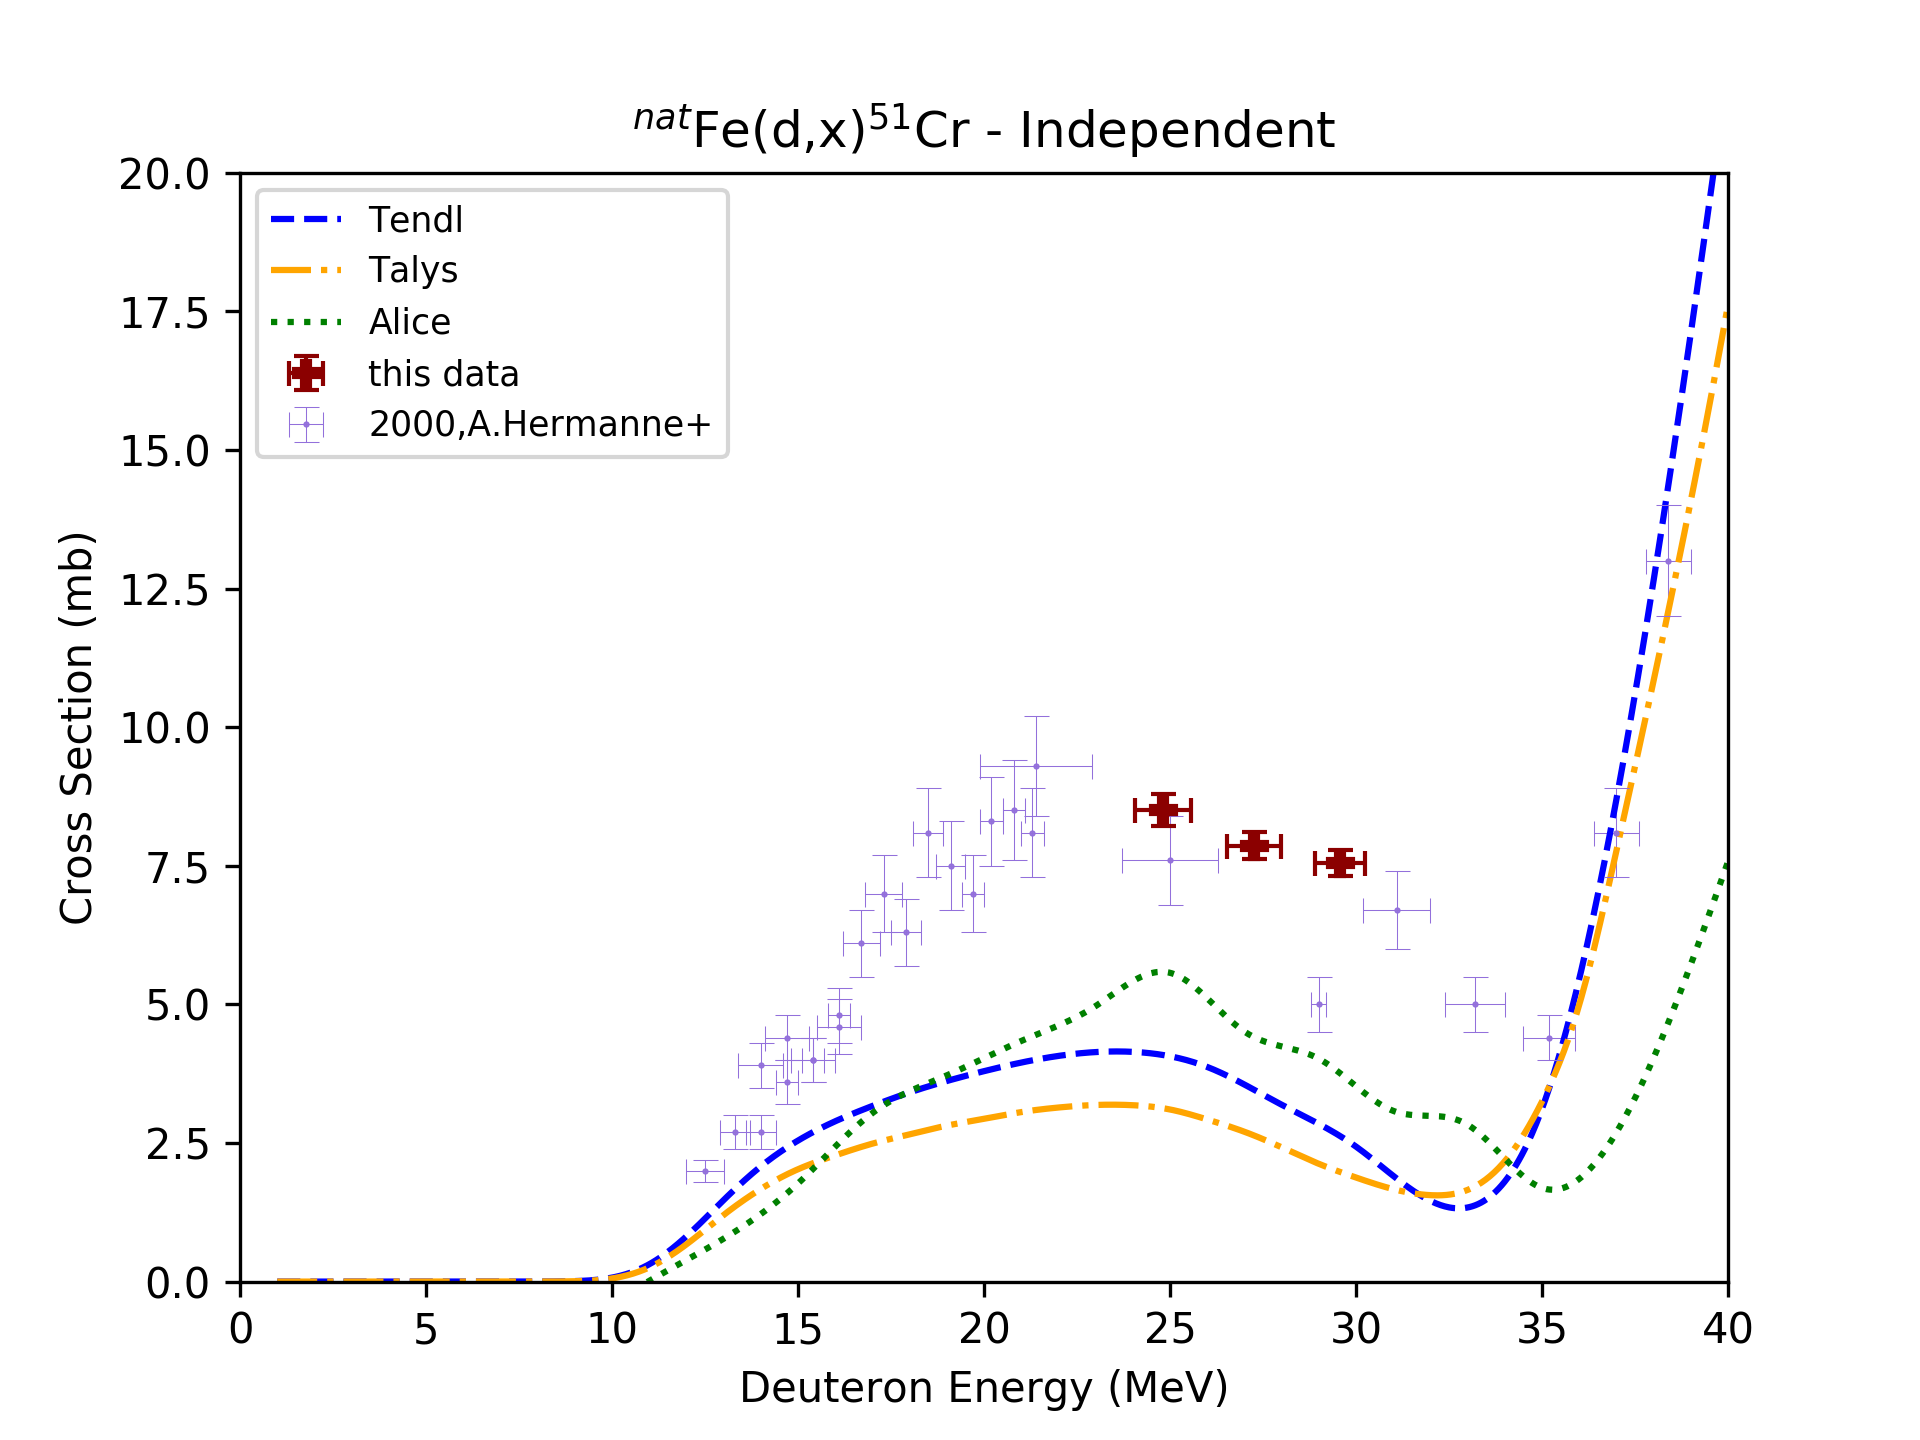
\includegraphics[width=8cm]{Results/Fe_51Cr.png} }}%
    \quad
    \subfloat[A cumulative measurement of $^{52}$Mn isomer (IT: 98.25\%) and groundstate. ]{{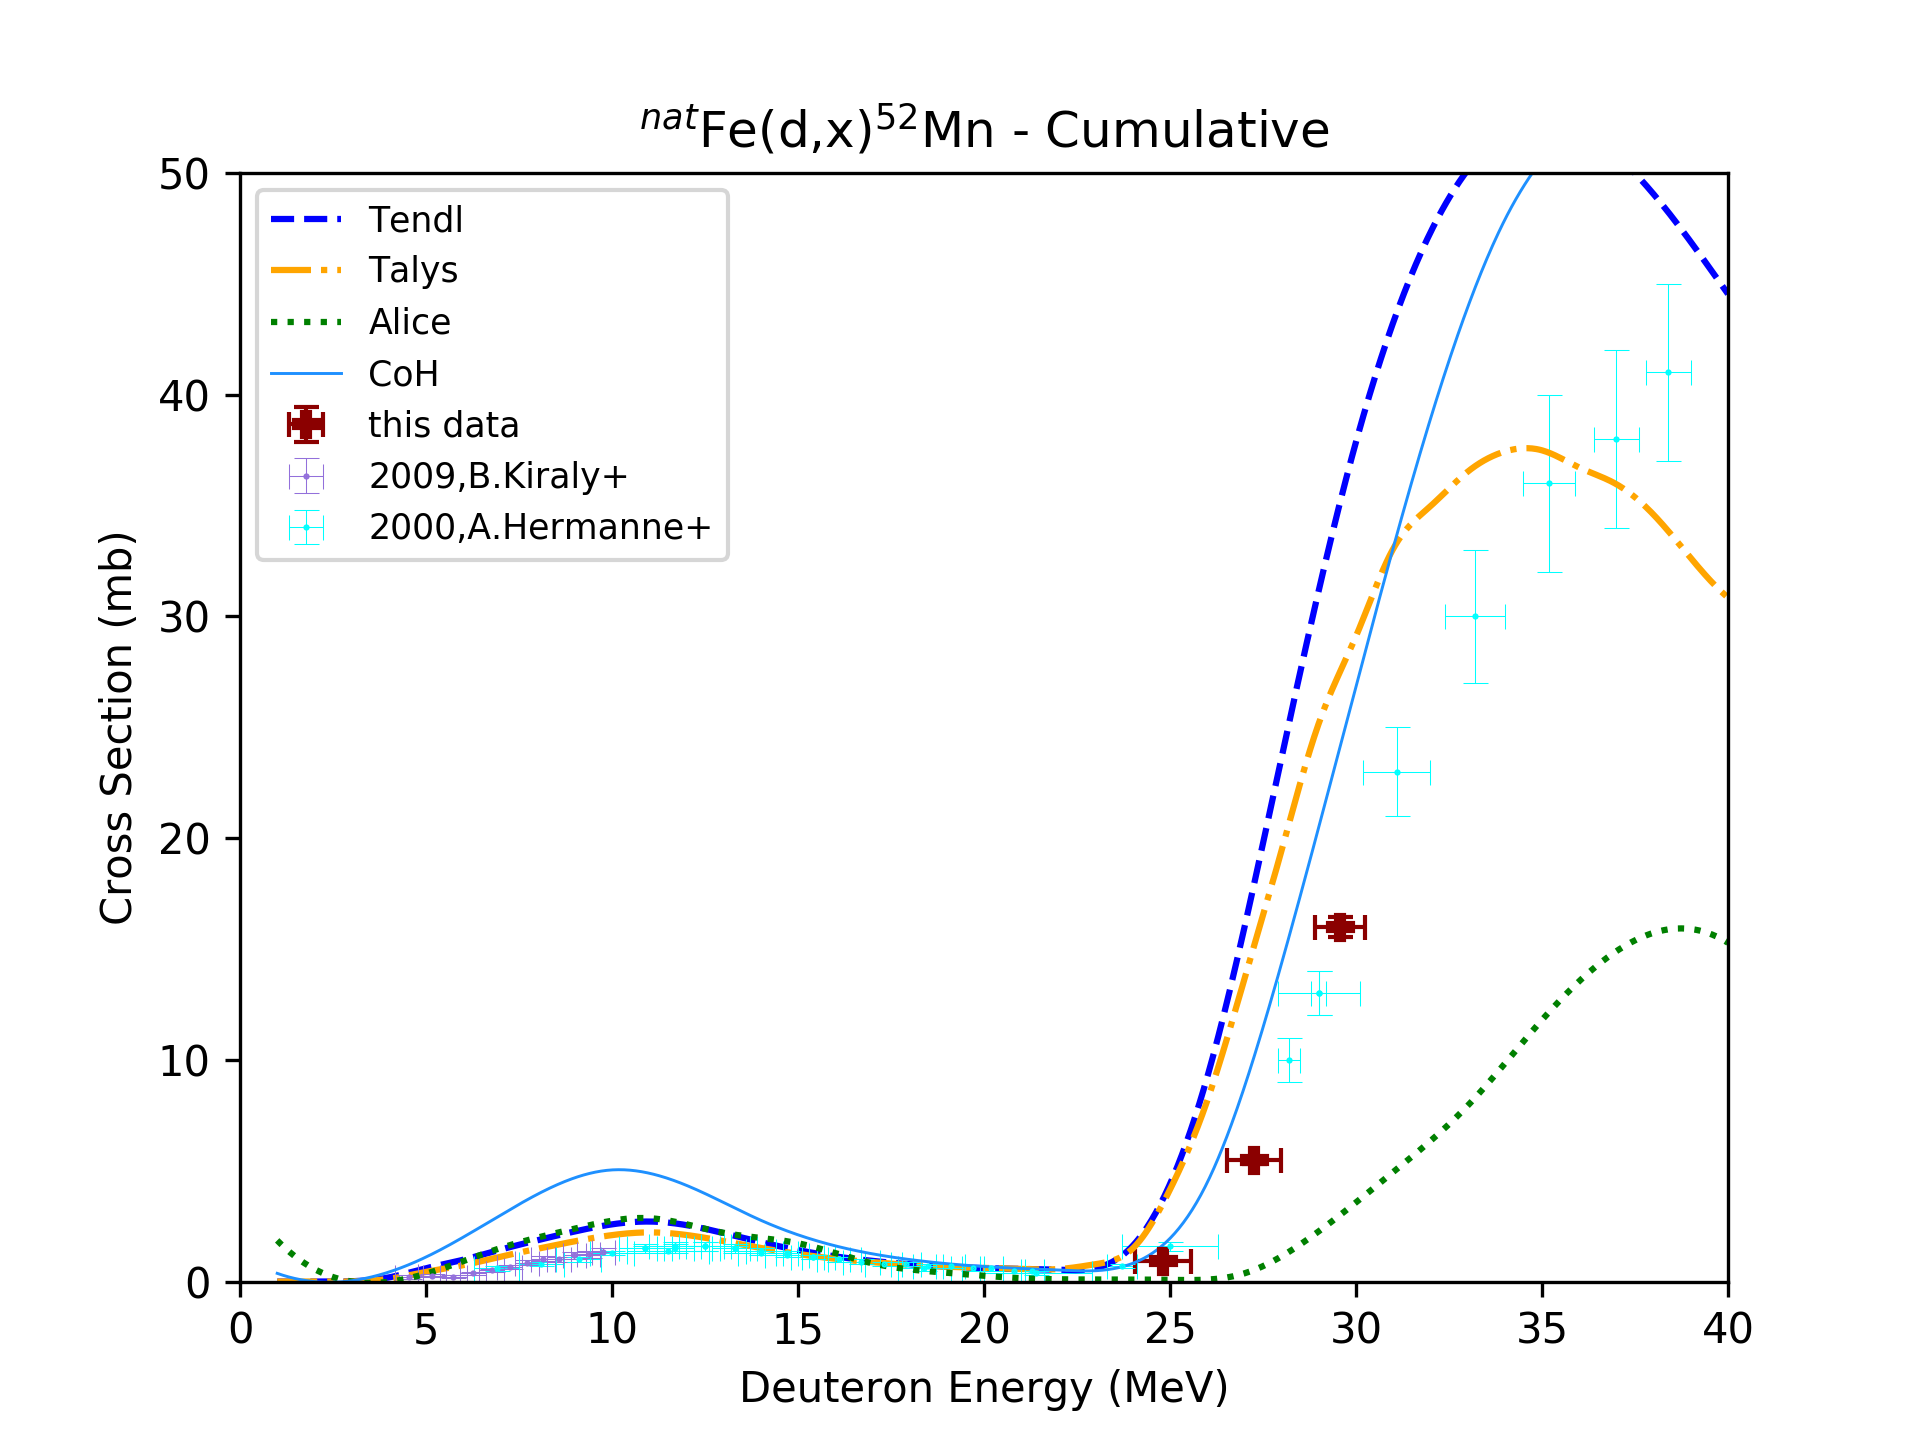
\includegraphics[width=8cm]{Results/Fe_52Mn.png} }}%
    \quad
    \subfloat[An independent measurement of $^{54}$Mn.]{{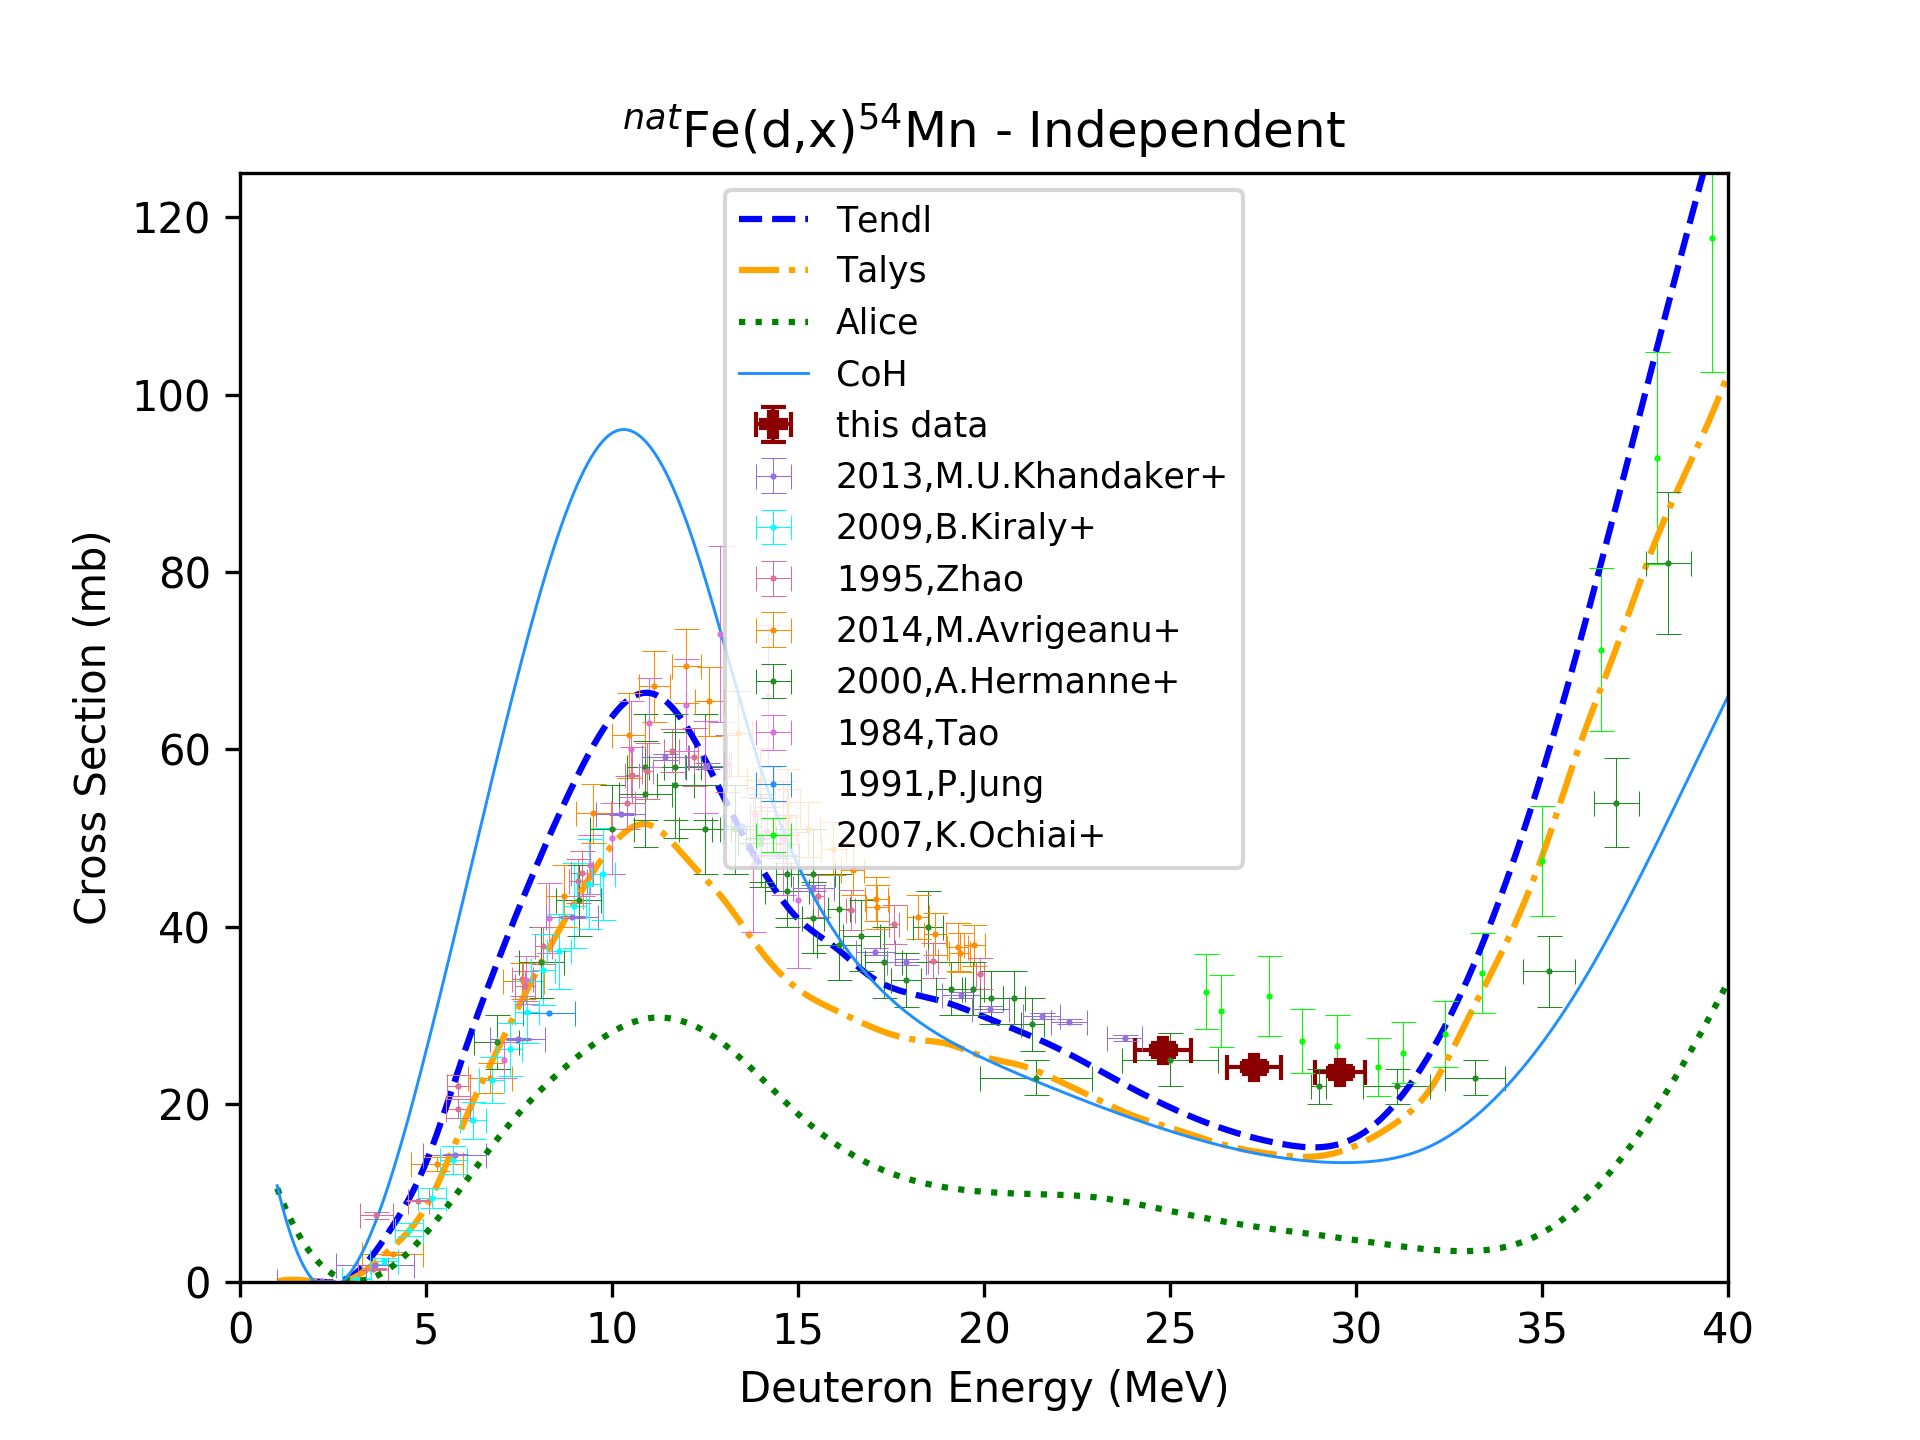
\includegraphics[width=8cm]{Results/Fe_54Mn.png} }}%
    \quad
    \subfloat[A cumulative measurement of $^{53}$Fe. ]{{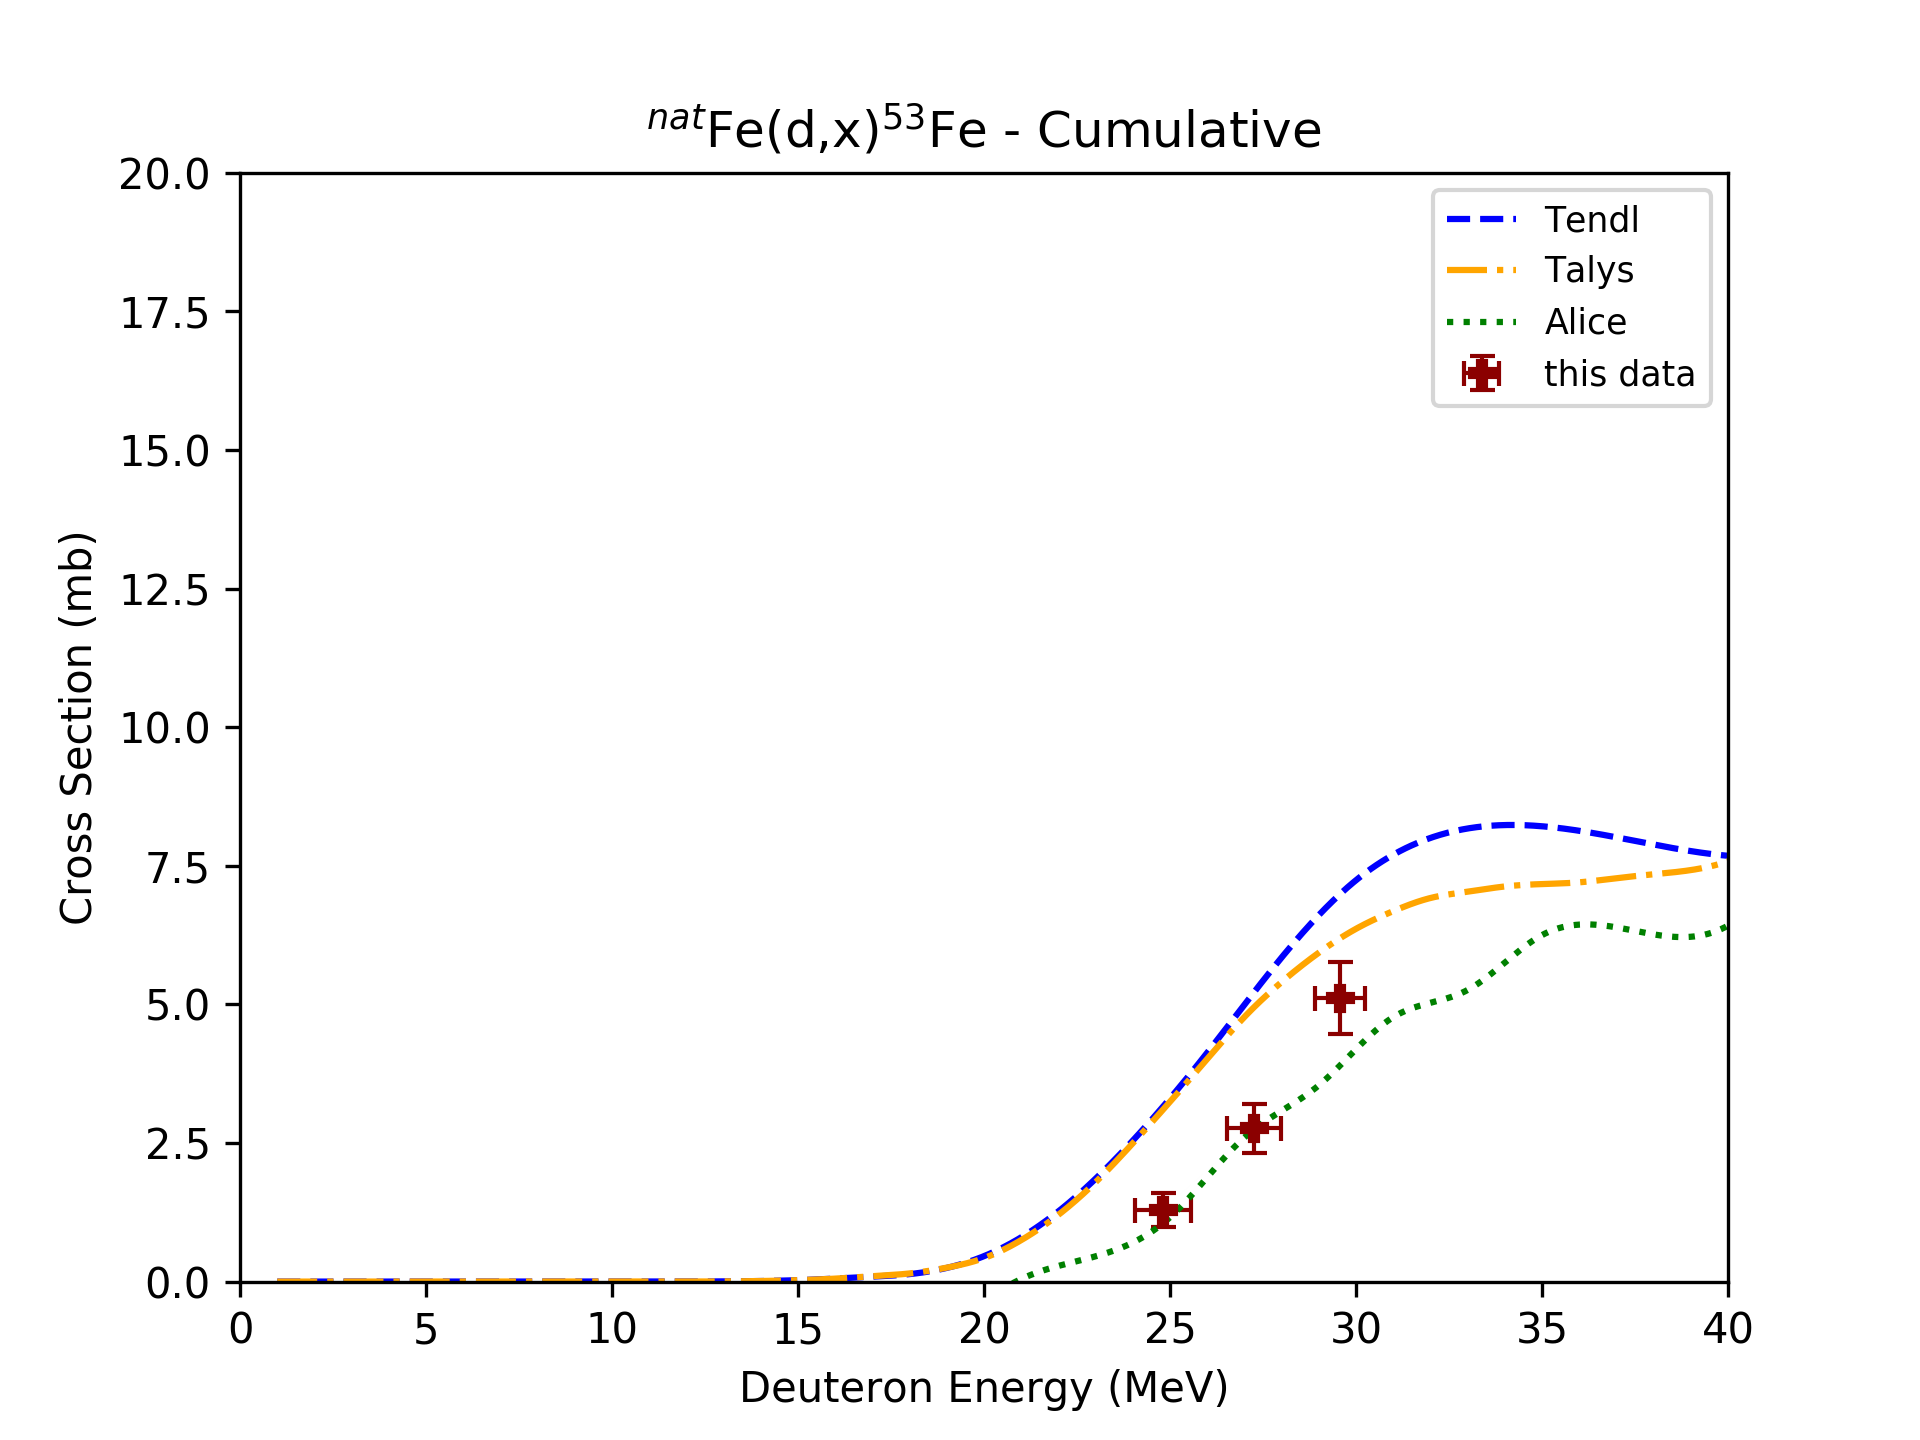
\includegraphics[width=8cm]{Results/Fe_53Fe.png} }}%
    \quad
      \caption{Excitation functions for $^{48}$V, $^{51}$Cr, $^{52}$Mn, $^{54}$Mn, $^{53}$Fe produced from iron.  }%
    \label{fig:cross-sections_188,189Ir}%
\end{figure} 

\begin{figure}%
    \centering
    \subfloat[An independent measurement of $^{59}$Fe. ]{{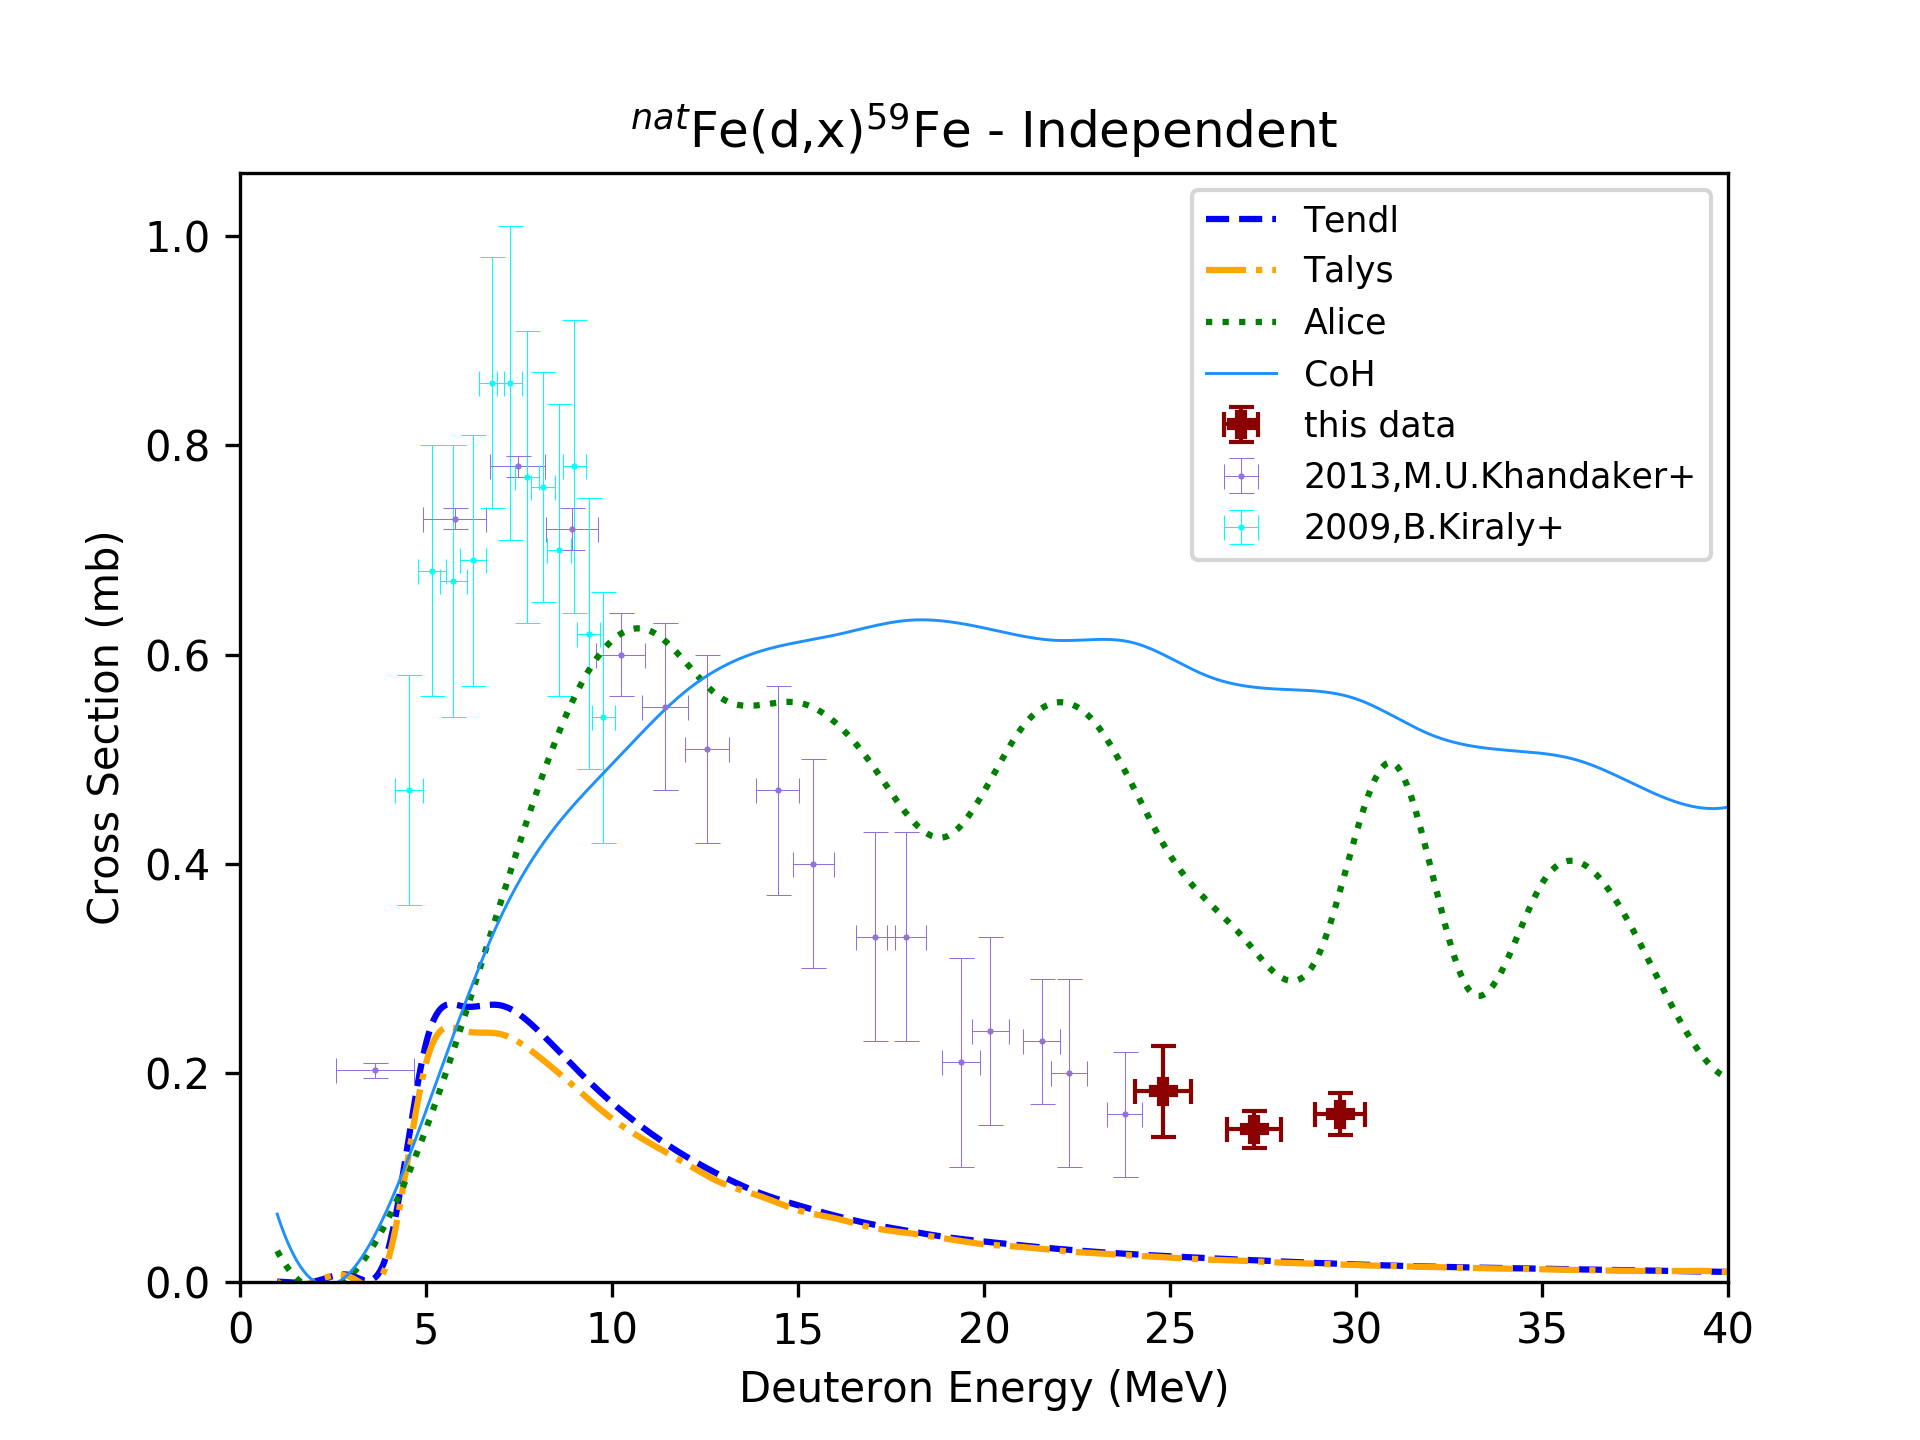
\includegraphics[width=8cm]{Results/Fe_59Fe.png} }}%
    \quad
    \subfloat[An independent measurement of $^{55}$Co. ]{{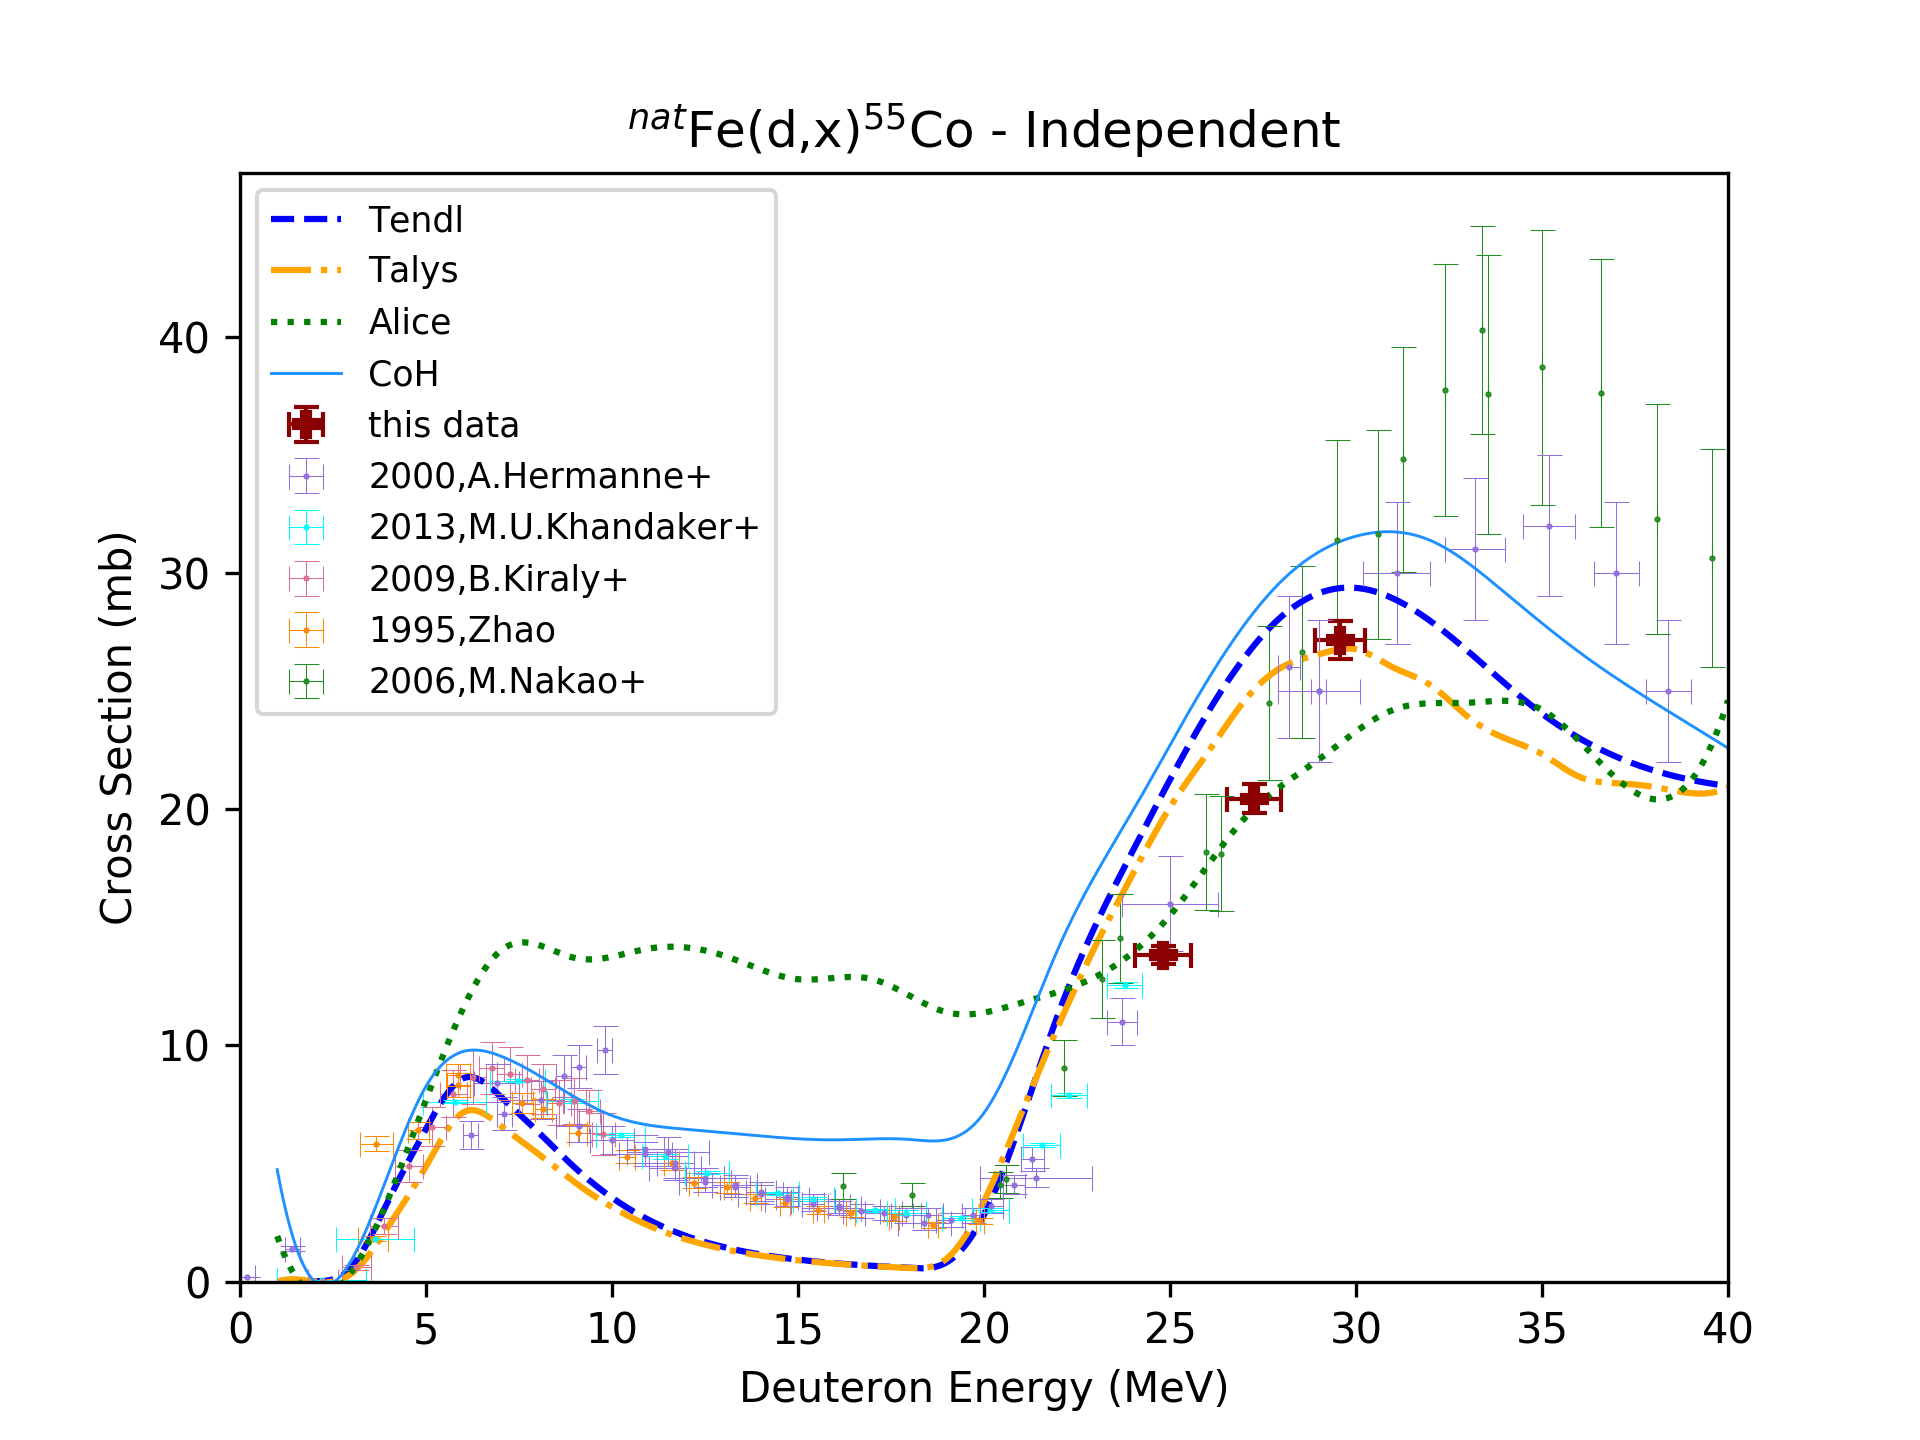
\includegraphics[width=8cm]{Results/Fe_55Co.png} }}%
    \quad
    \subfloat[An independent measurement of $^{57}$Co. ]{{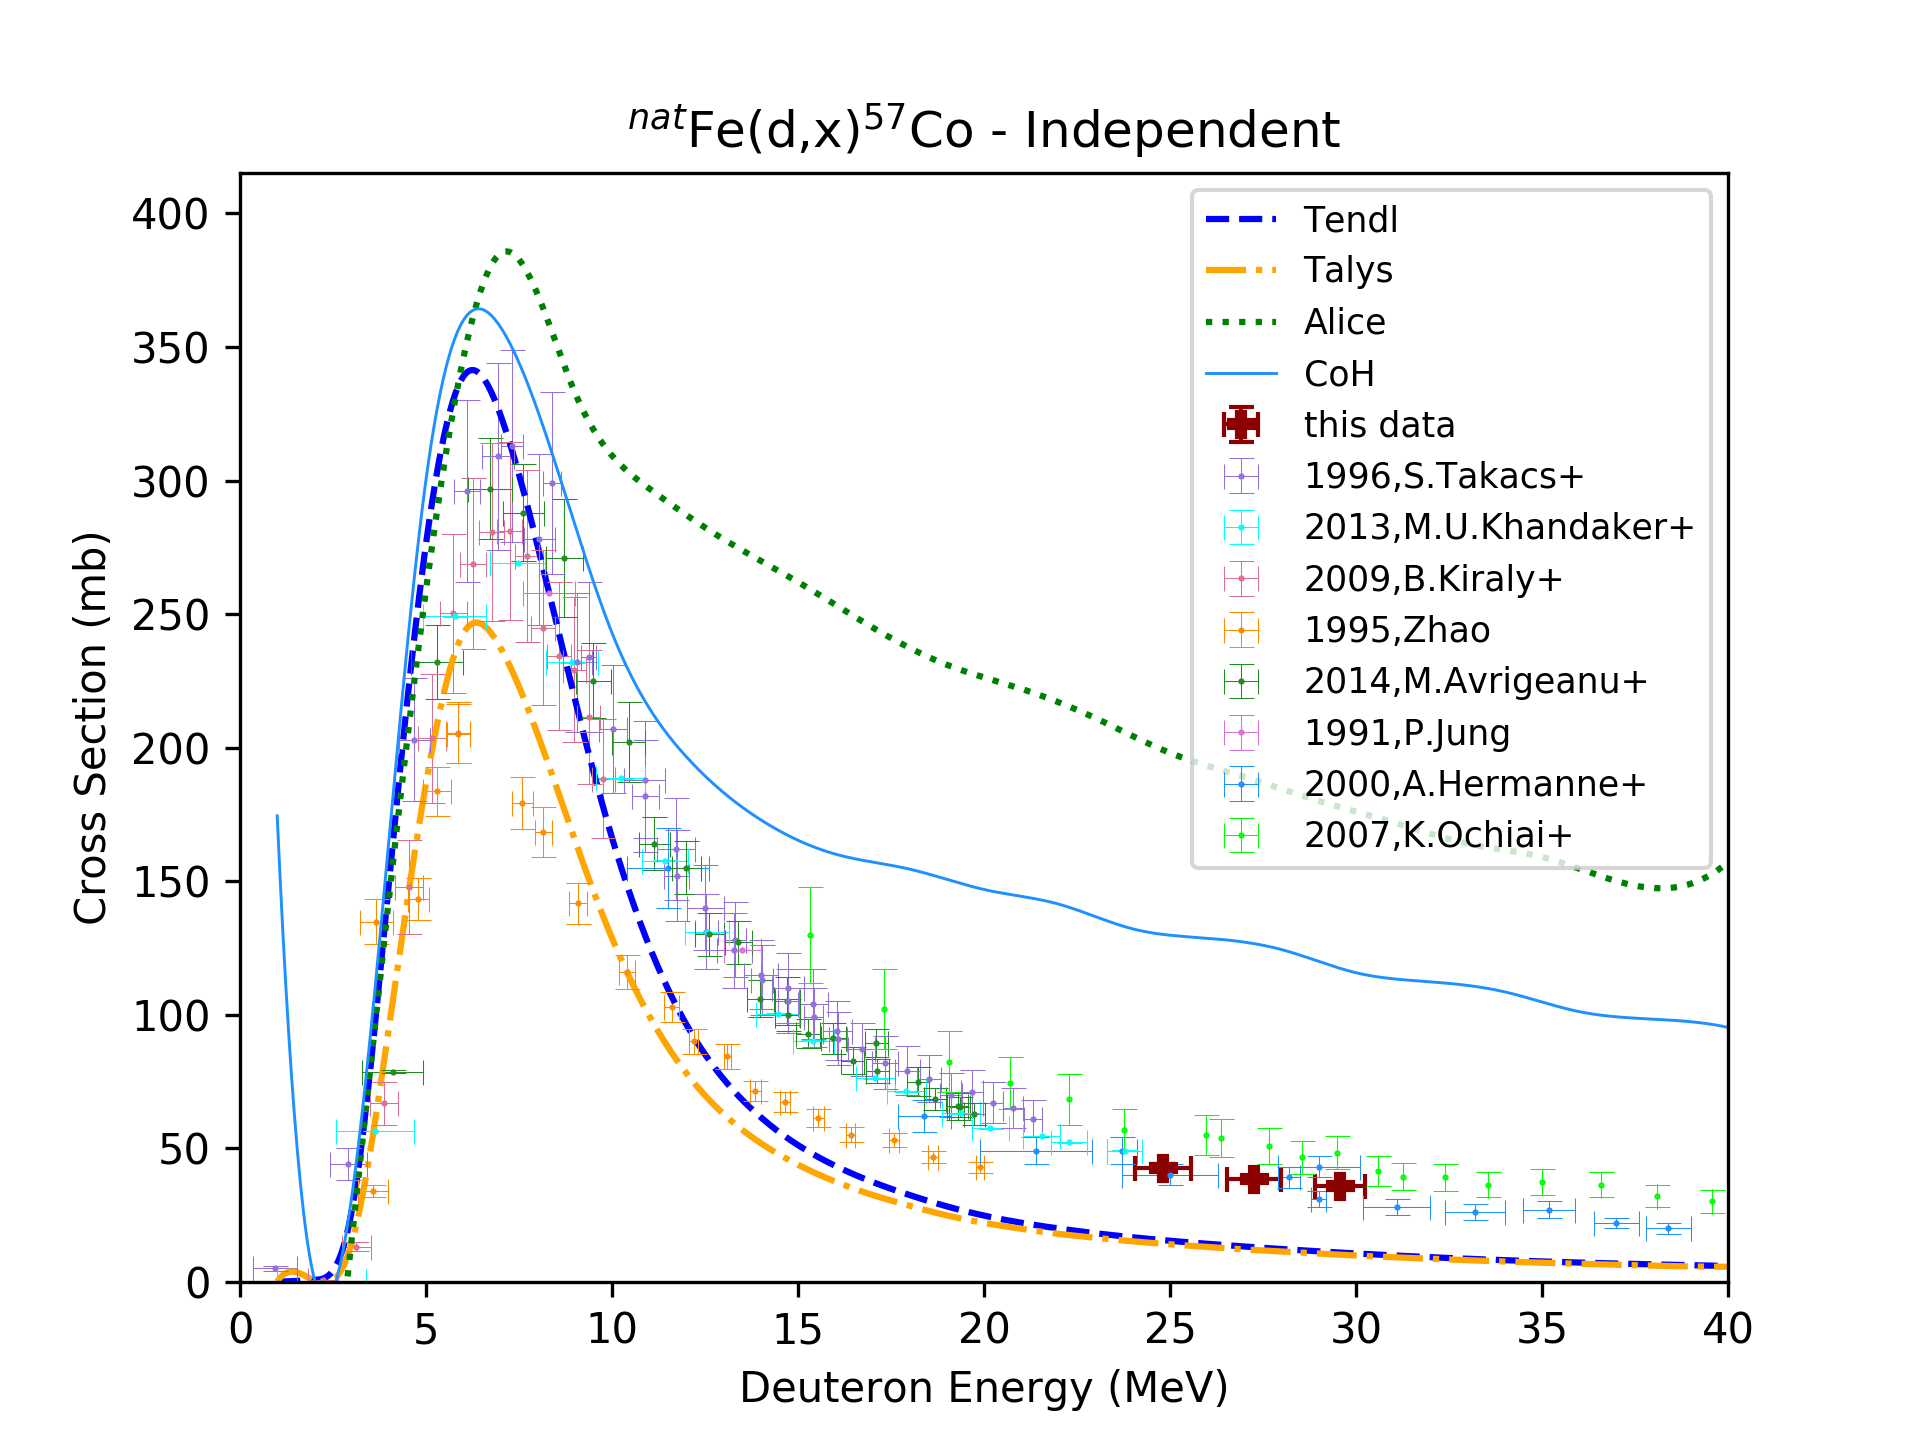
\includegraphics[width=8cm]{Results/Fe_57Co.png} }}%
    \quad
    \subfloat[An independent measurement of $^{58}$Co. ]{{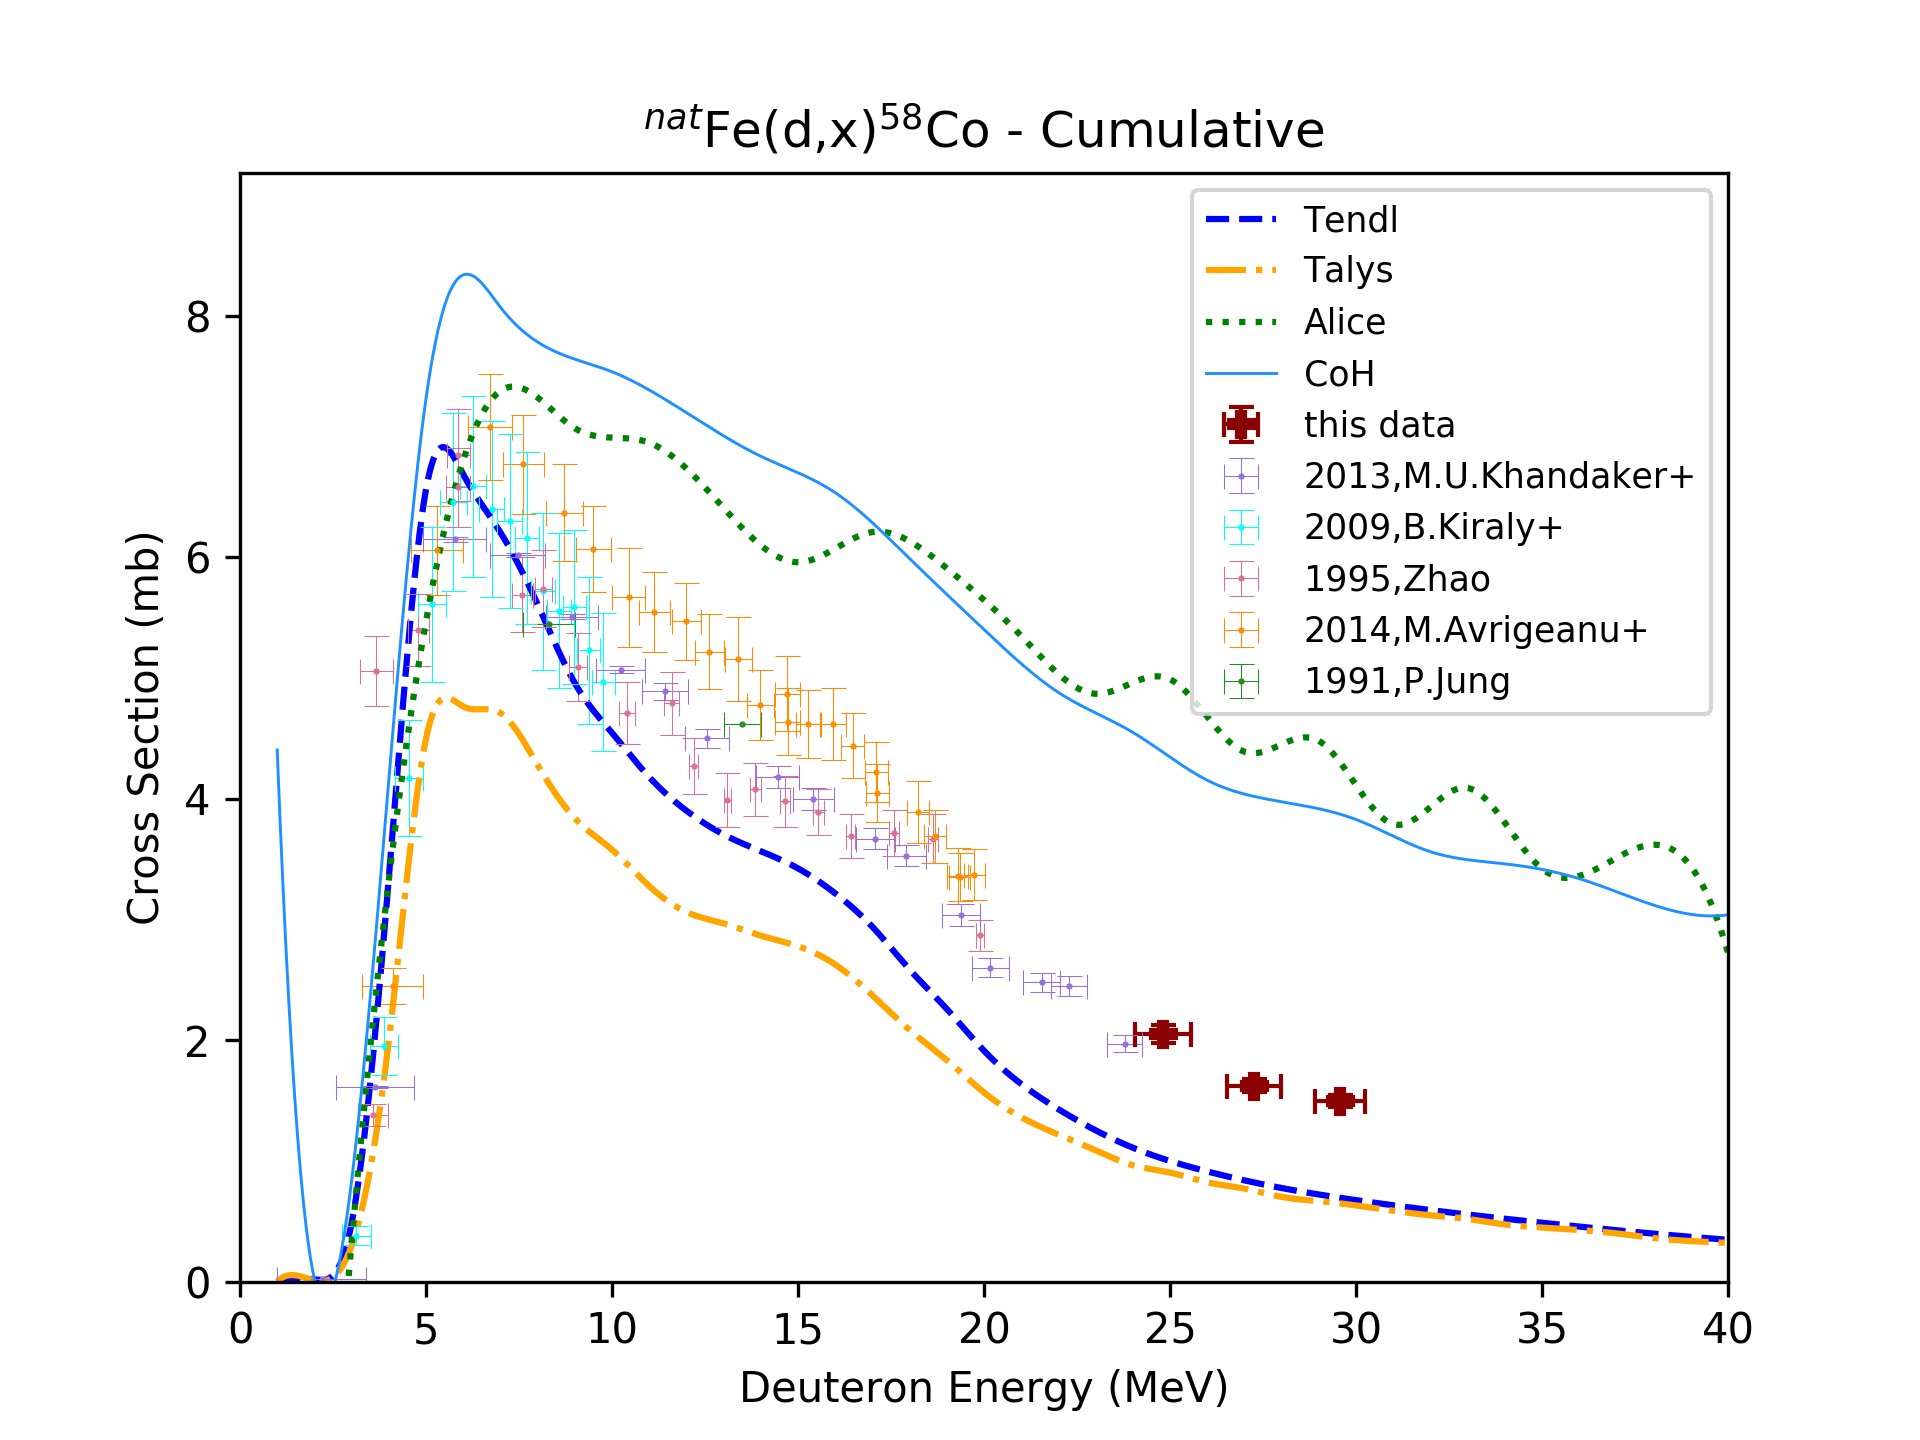
\includegraphics[width=8cm]{Results/Fe_58Co.png} }}%
    \quad
      \caption{Excitation functions for $^{59}$Fe, $^{55}$Co, $^{57}$Co, $^{58}$Co produced from iron.  }%
    \label{fig:cross-sections_188,189Ir}%
\end{figure} 

\begin{figure}%
    \centering
    \subfloat[A cumulative measurement of $^{59}$Fe]{{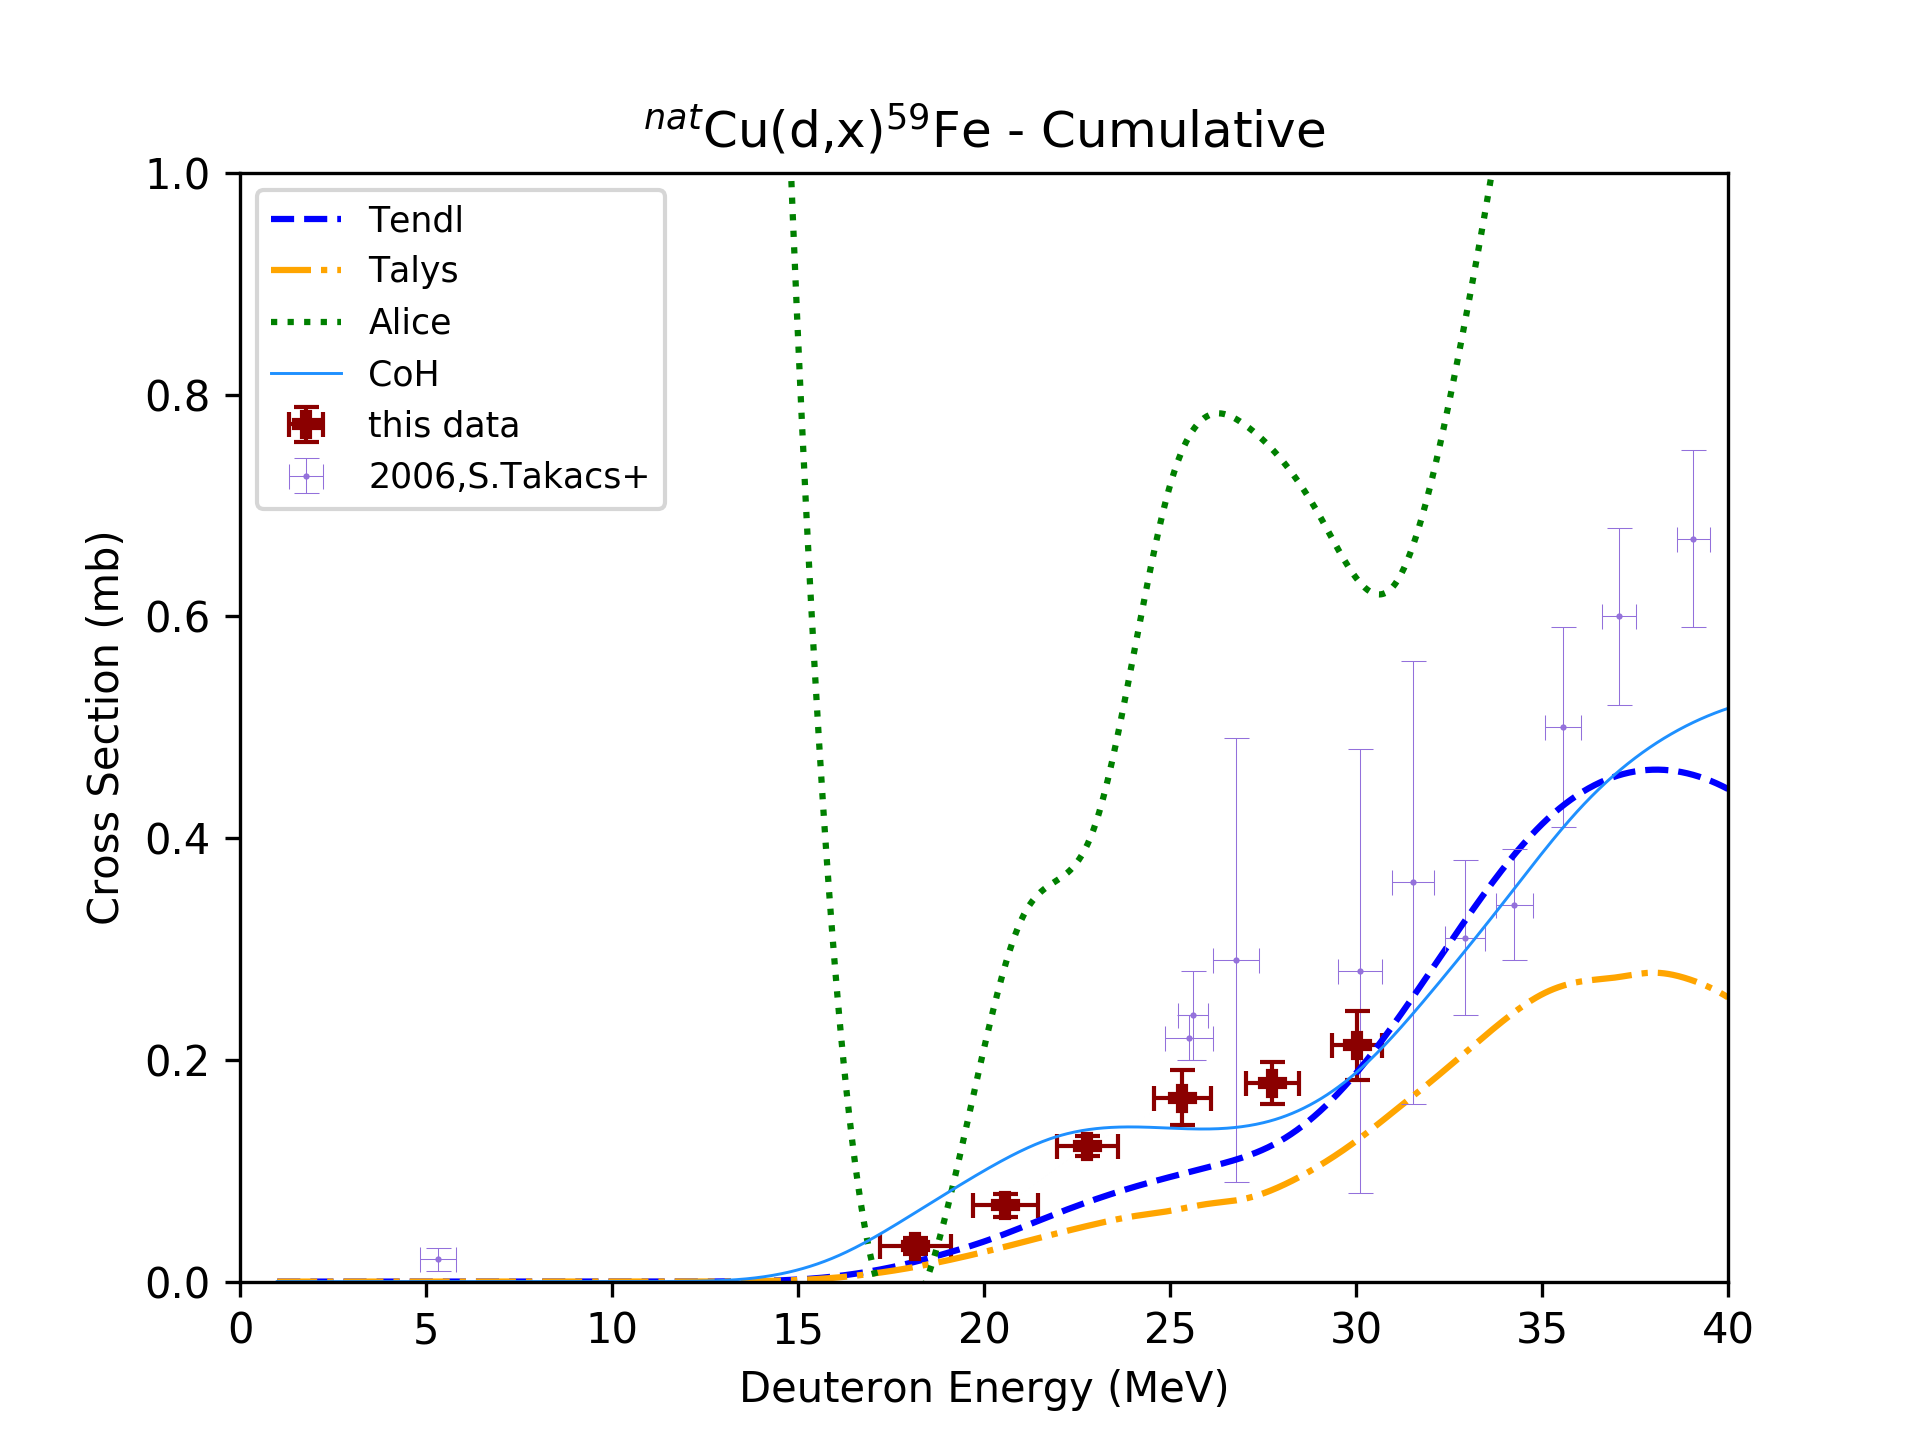
\includegraphics[width=8cm]{Results/Cu_59Fe.png} }}%
    \quad
    \subfloat[A cumulative measurement of $^{60}$Co of isomer (IT:99.75\%) and groundstate. ]{{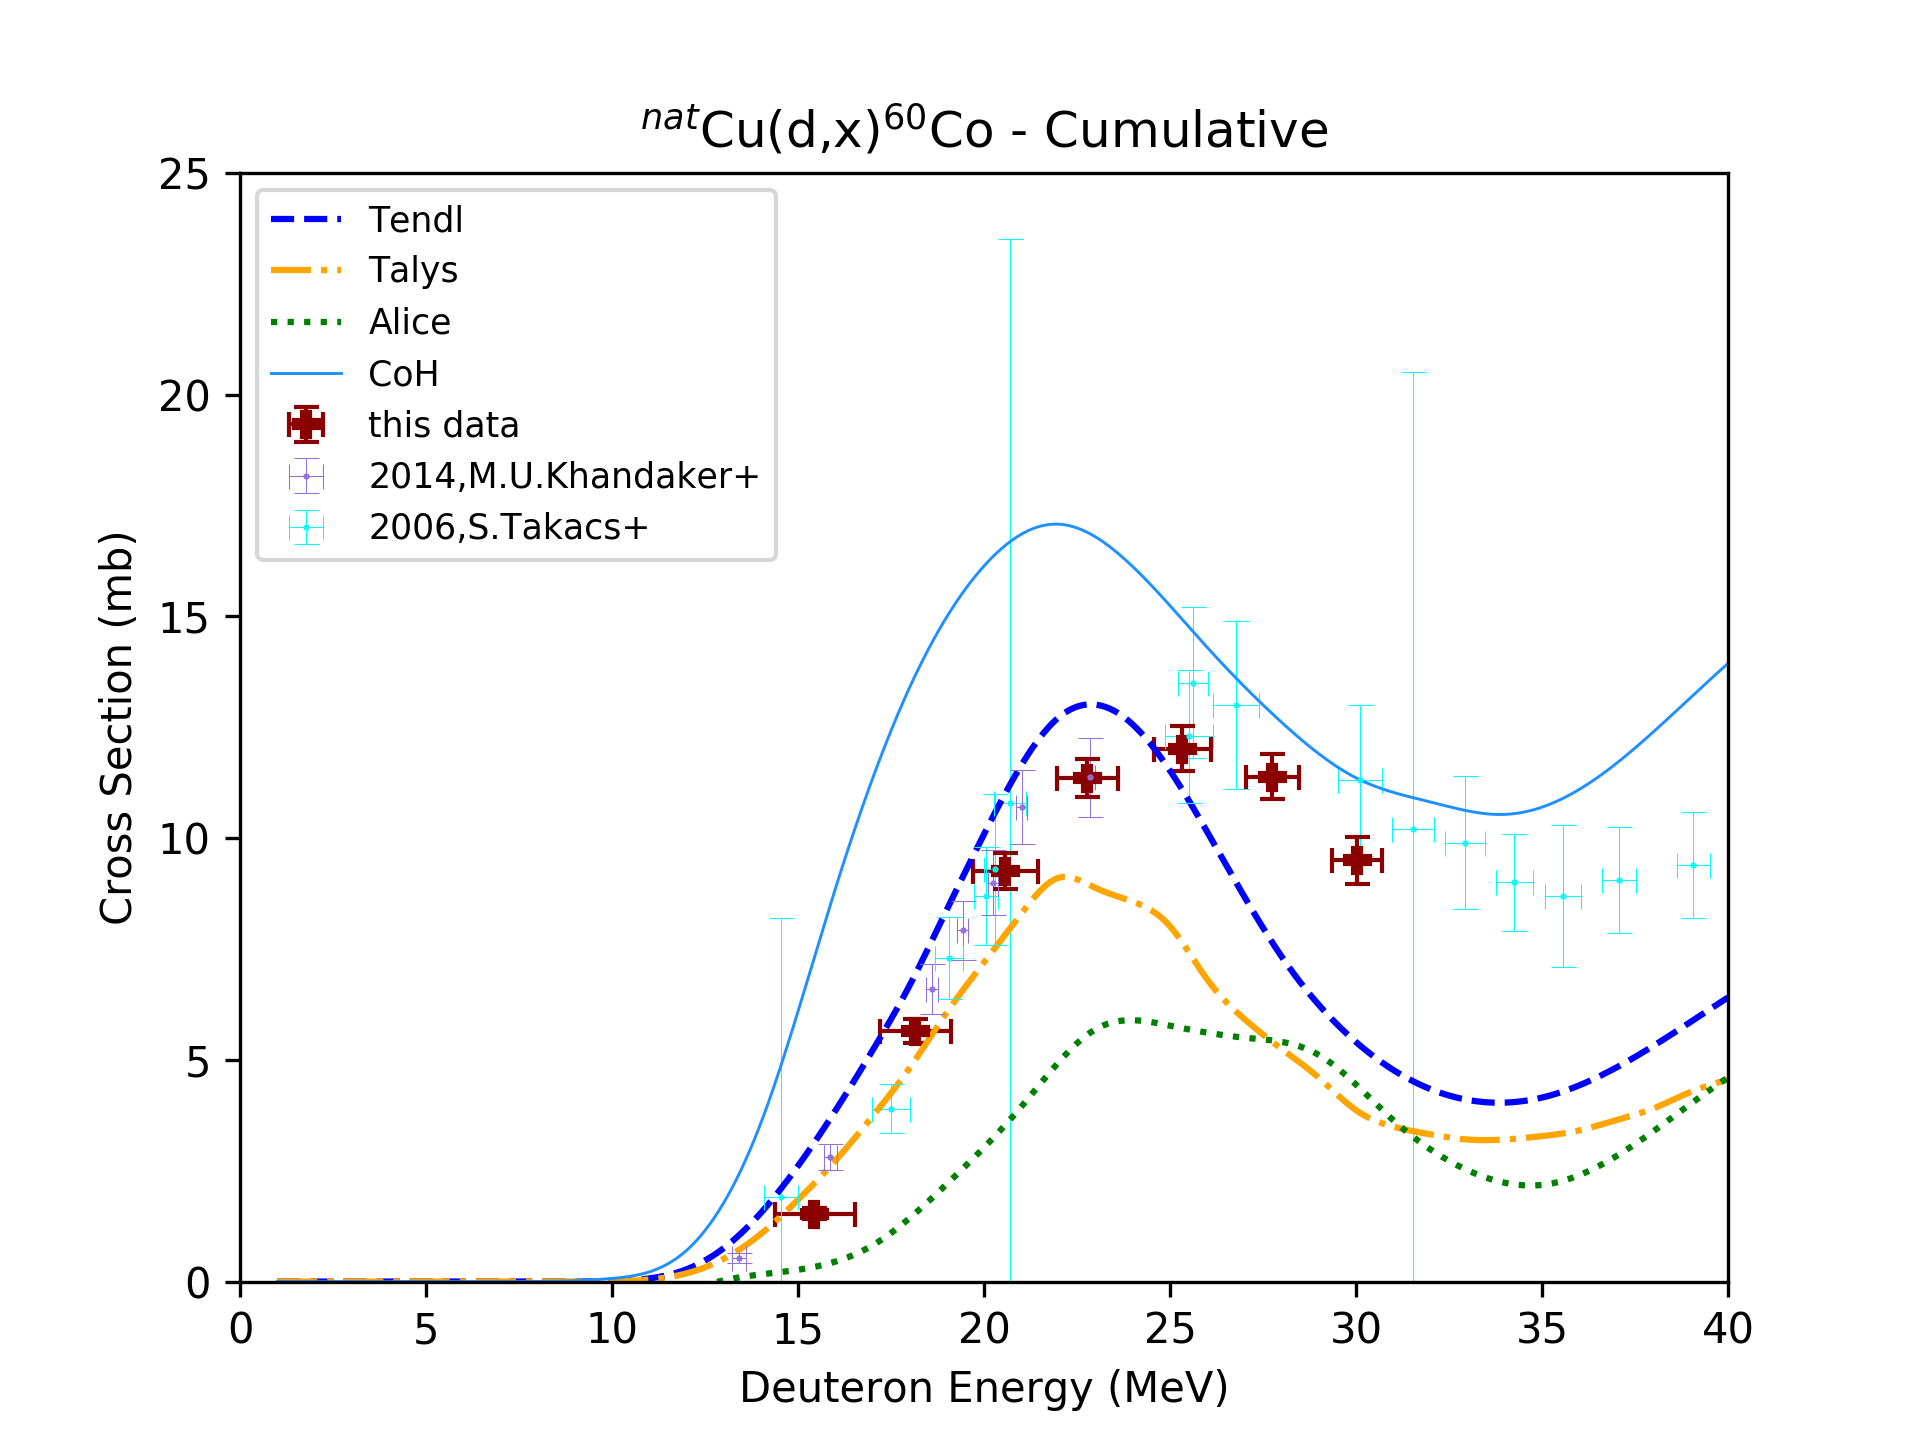
\includegraphics[width=8cm]{Results/Cu_60Co.png} }}%
    \quad
    \subfloat[A cumulative measurement of $^{61}$Co. ]{{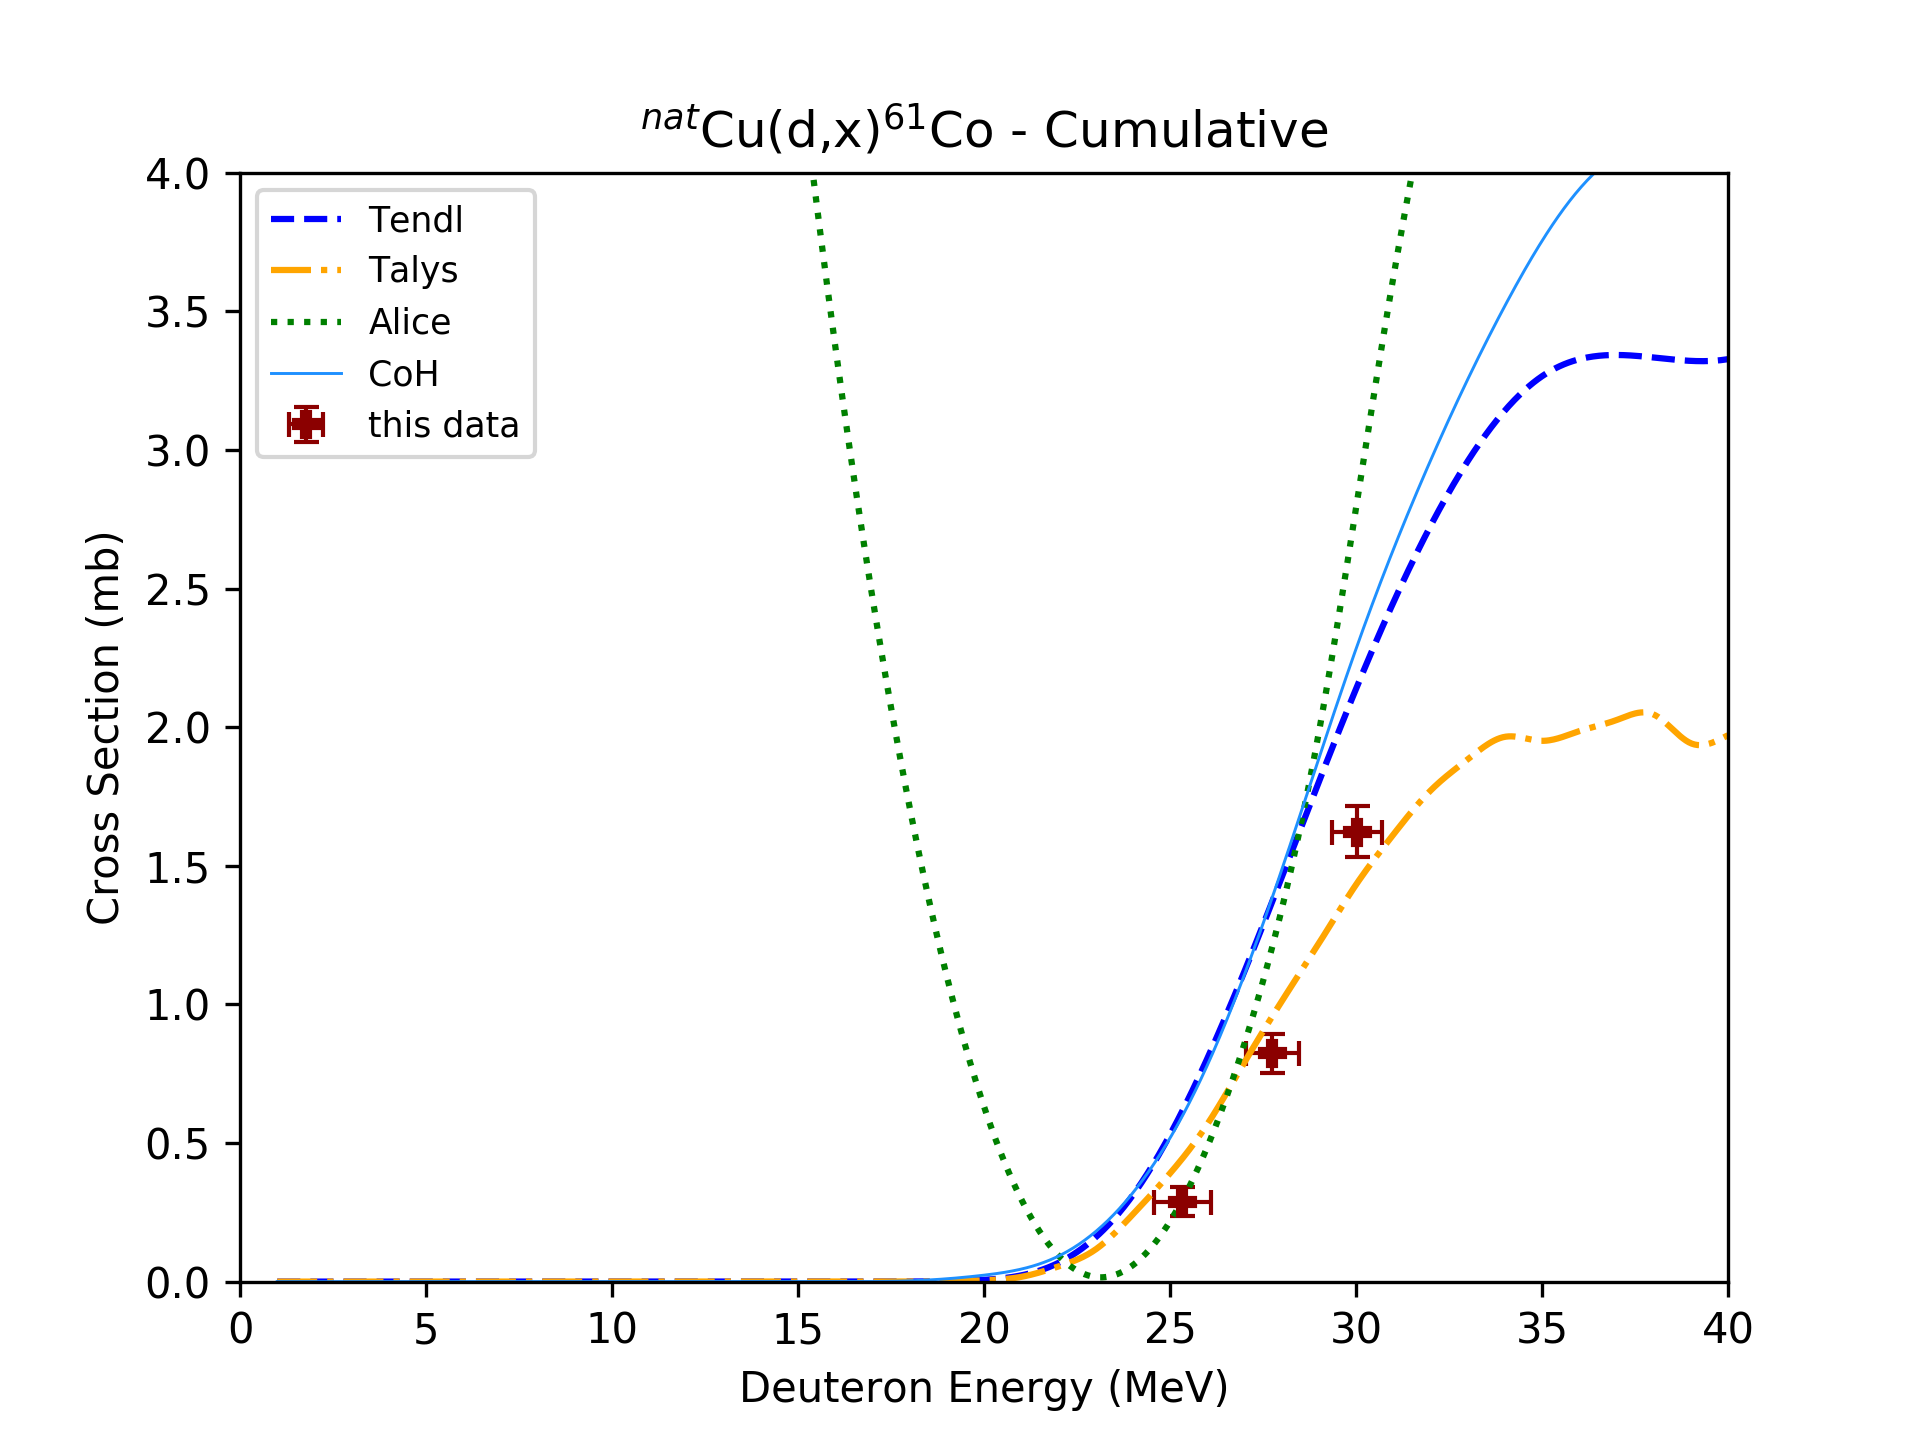
\includegraphics[width=8cm]{Results/Cu_61Co.png} }}%
    \quad
    \subfloat[An independent measurement of $^{65}$Ni.]{{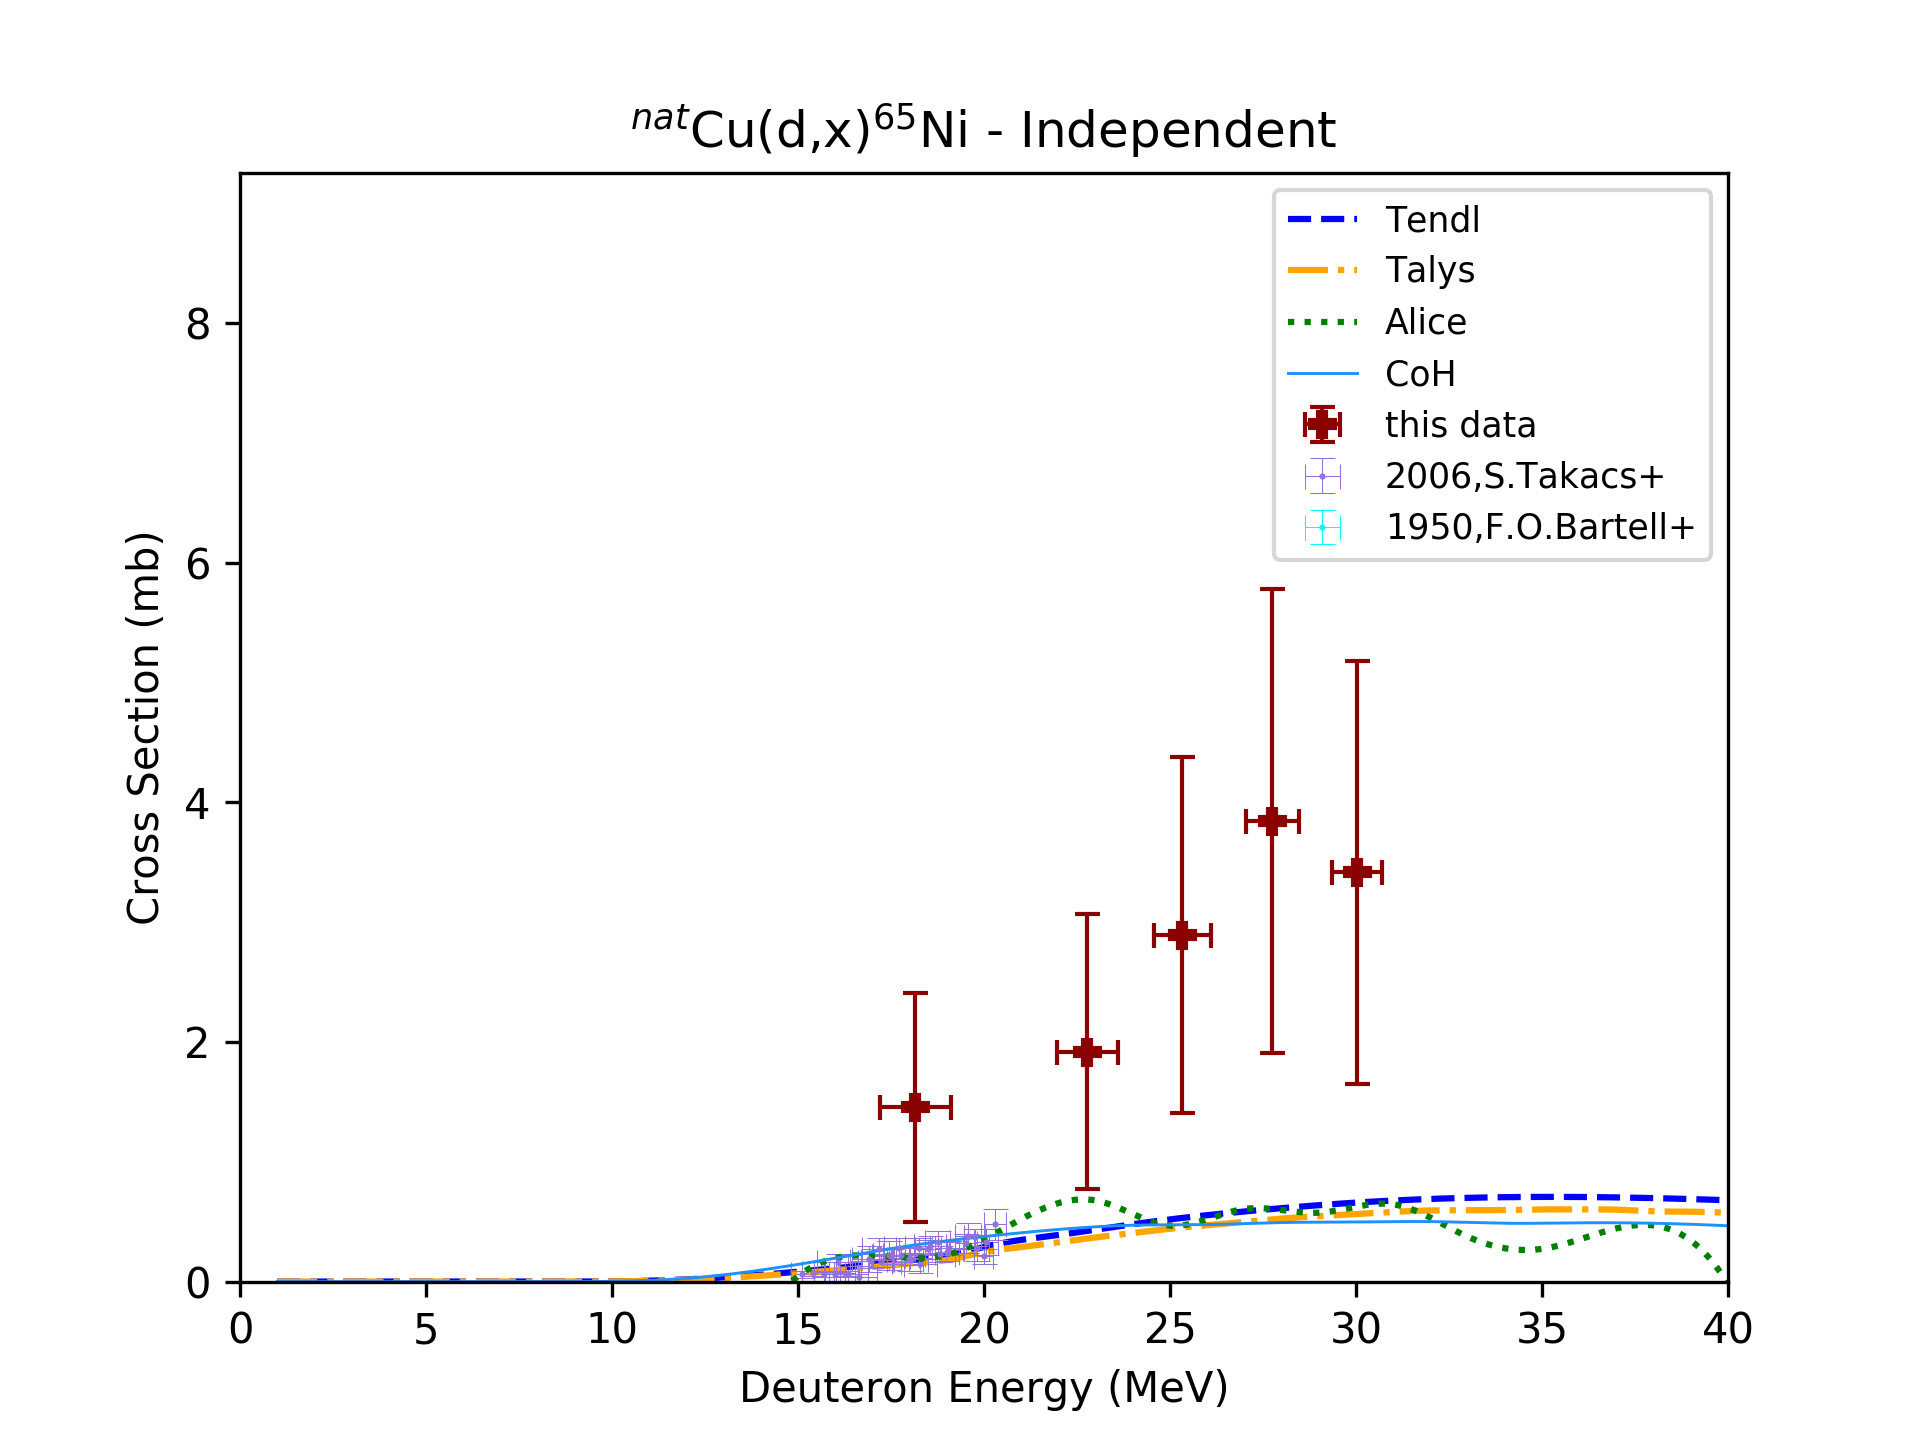
\includegraphics[width=8cm]{Results/Cu_65Ni.png} }}%
    \quad
    \subfloat[A cumulative measurement of $^{62}$Cu.]{{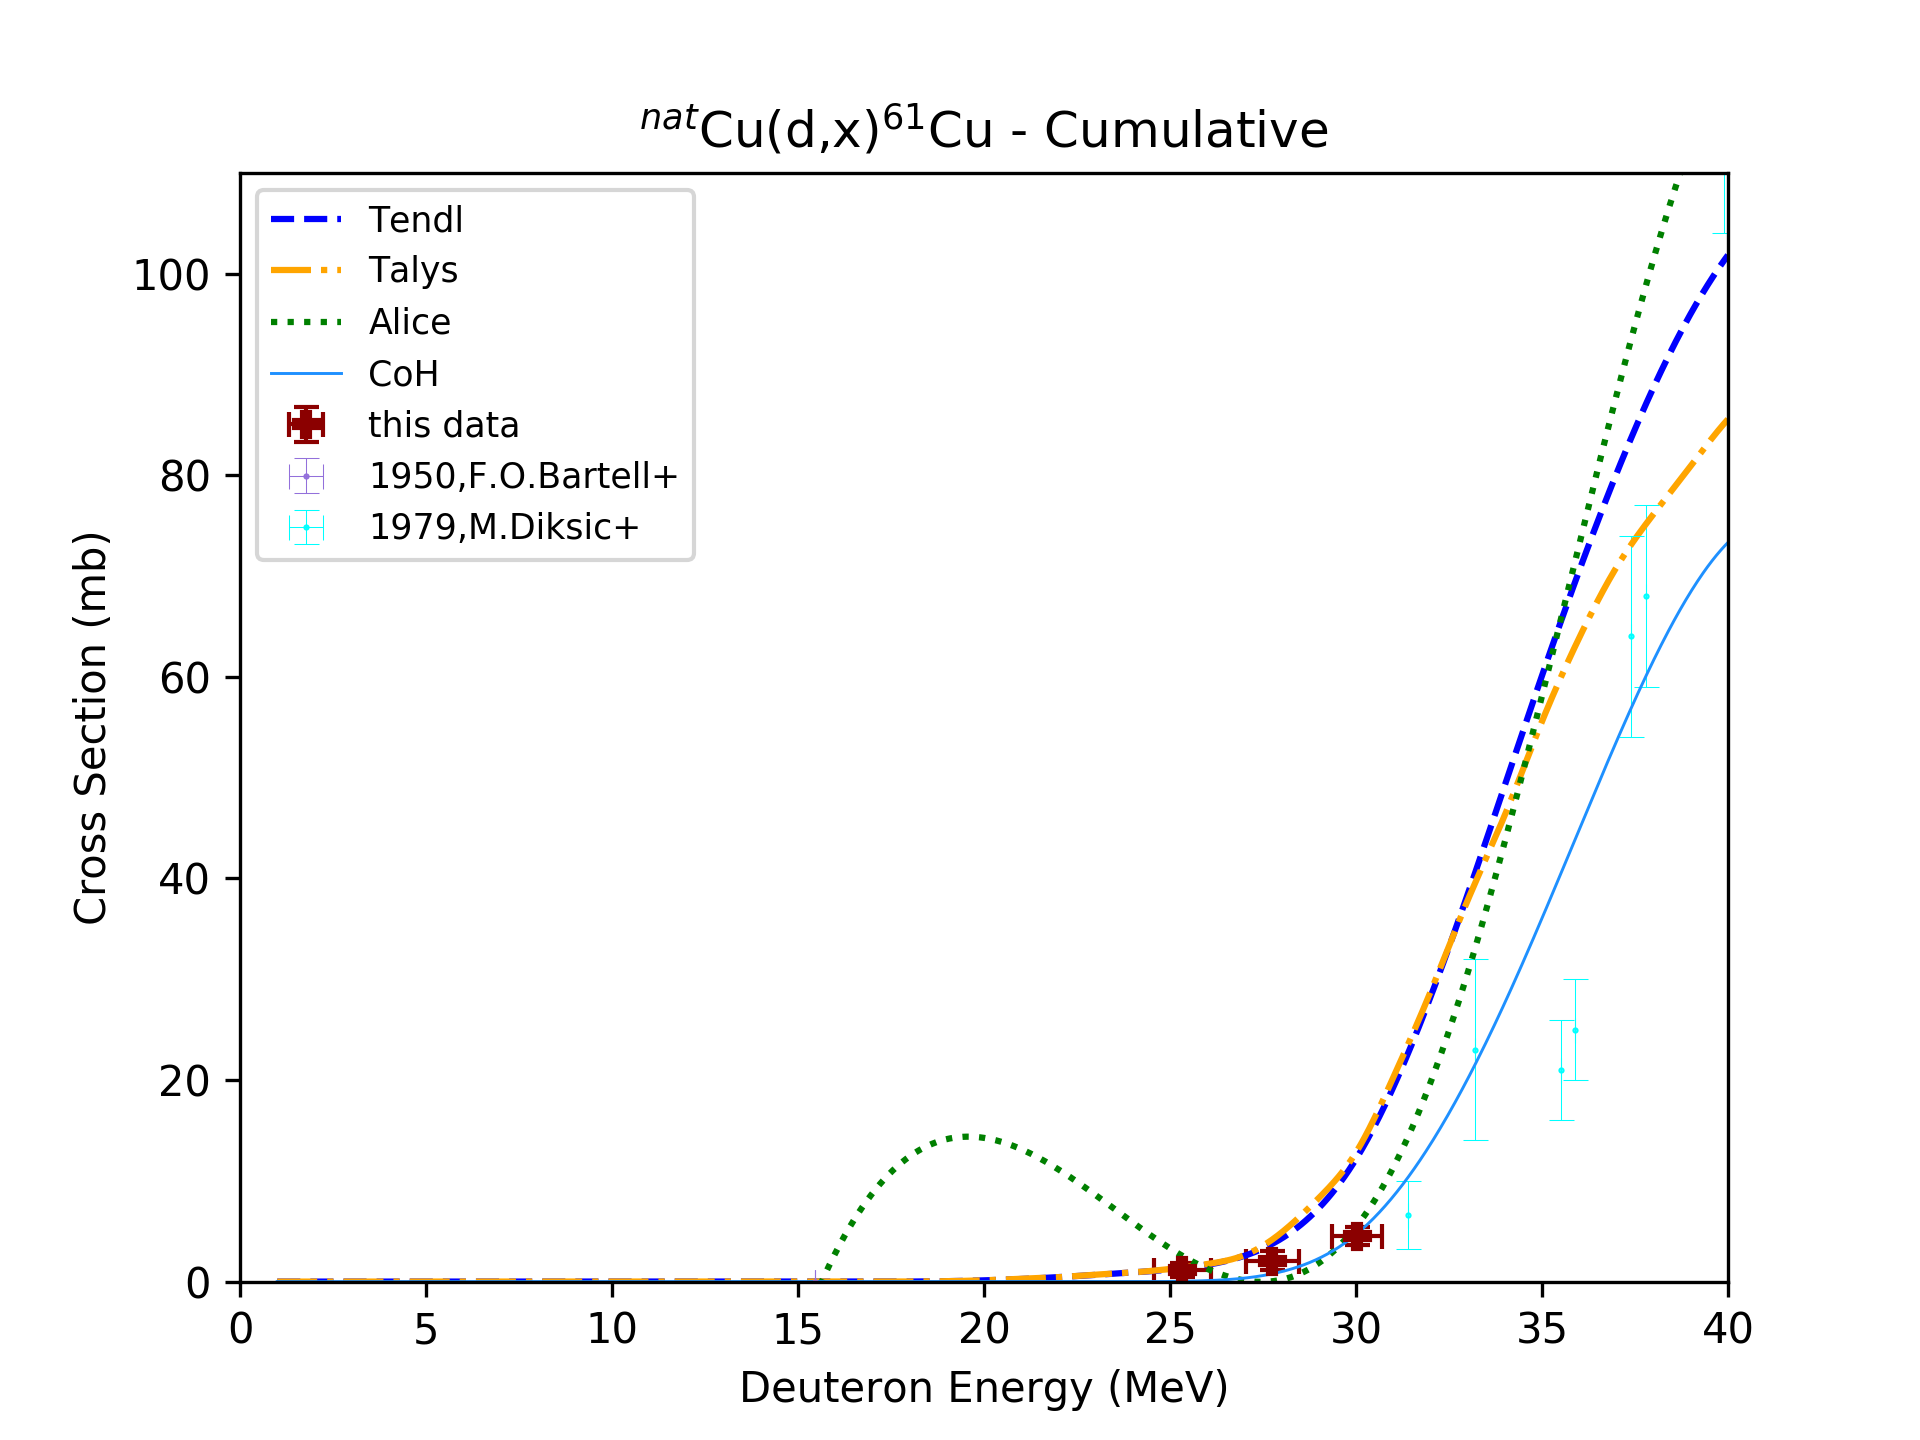
\includegraphics[width=8cm]{Results/Cu_61Cu.png} }}%
    \quad
    \subfloat[An independent measurement of $^{64}$Cu.]{{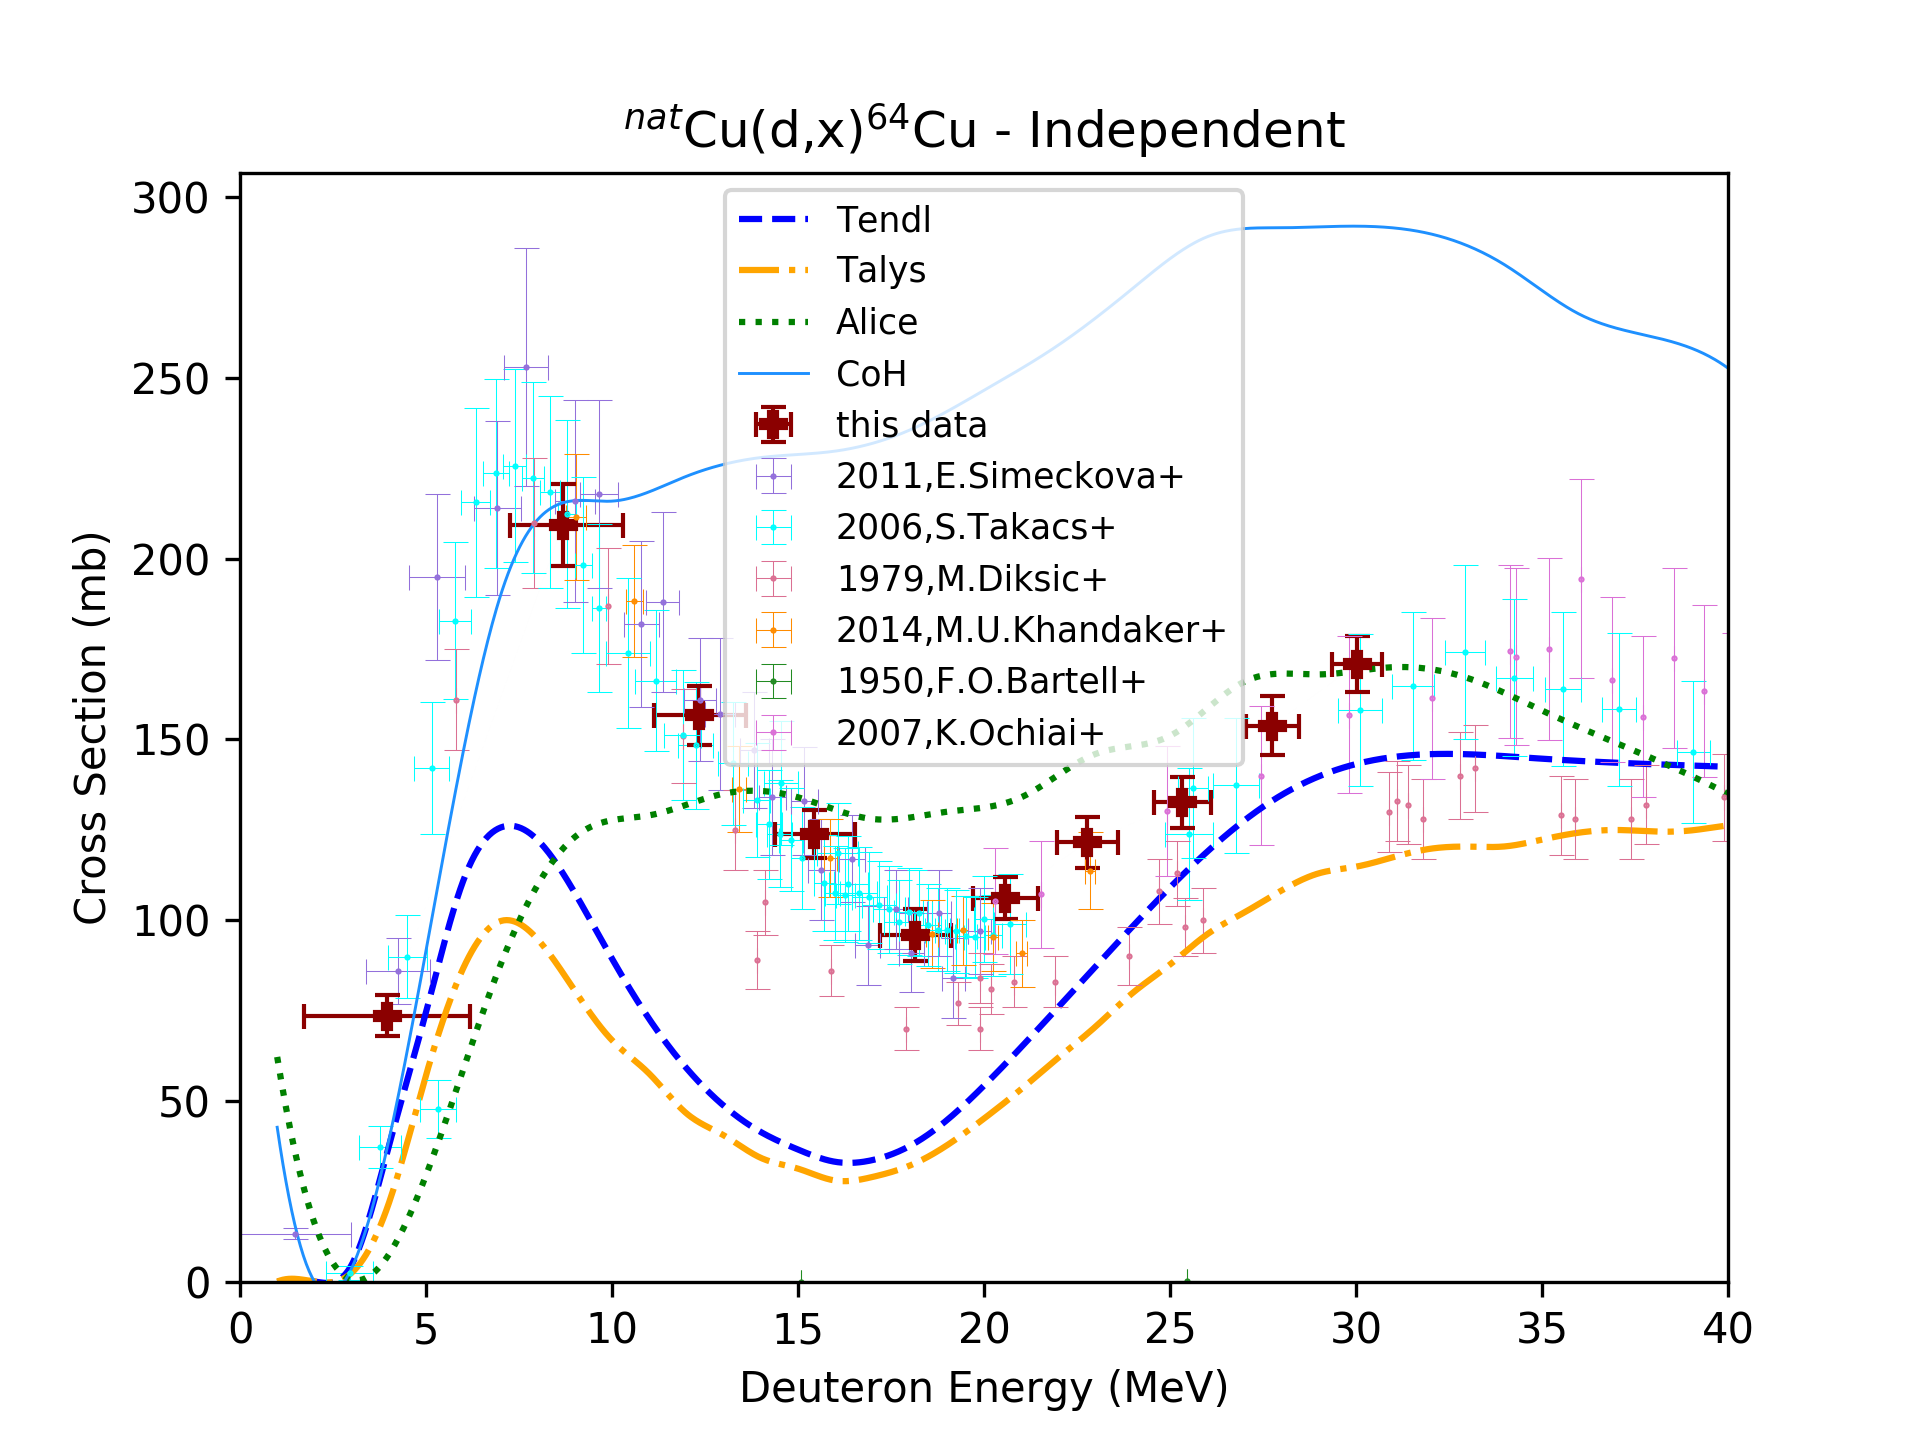
\includegraphics[width=8cm]{Results/Cu_64Cu.png} }}%
    \quad
      \caption{Excitation functions for $^{59}$Fe, $^{55}$Co, $^{57}$Co, $^{58}$Co produced from iron.  }%
    \label{fig:cross-sections_188,189Ir}%
\end{figure} 




\begin{comment}
\begin{table}[]
    \centering
    \footnotesize
    \begin{tabular}{c c c c c c c c c c c} 
        \hline
       \makecell{E_d (MeV)}  &  \makecell{30.65_{-0.75}^{+0.76}} & \makecell{28.40_{-0.79}^{+0.80}} & \makecell{26.03_{-0.82}^{+0.82}} & \makecell{23.54_{-0.87}^{+0.88}} & \makecell{21.38_{-0.92}^{+0.94}} & \makecell{19.03_{-0.99}^{+1.00}} & \makecell{16.43_{-1.08}^{+1.11}} & \makecell{13.51_{-1.22}^{+1.28}} & \makecell{10.09_{-1.41}^{+1.55}} & \makecell{5.63_{-1.83}^{+2.21}}   \\
       \hline
       
       \makecell{$^{188}$Ir} & \makecell{} & \makecell{} & \makecell{} &  \makecell{} &  \makecell{} &  \makecell{} &  \makecell{} &  \makecell{} &  \makecell{} &  \makecell{} \\
       \makecell{$^{193m}$Pt} & \makecell{48.11 \pm 6.33} & \makecell{} & \makecell{} &  \makecell{} &  \makecell{} &  \makecell{} &  \makecell{} &  \makecell{} &  \makecell{} &  \makecell{} \\       
       
    \end{tabular}
    \caption{Iridium cross sections. }
    \label{tab:my_label}
\end{table}



\newpage
\pagestyle{empty}
\begingroup
\setlength{\tabcolsep}{10pt} % Default value: 6pt
\renewcommand{\arraystretch}{1.2} % Default value: 1
%\begin{landscape}
%\begin{table}[]
\begin{sidewaystable}
    \centering
    \small
    \begin{tabular}{c c c c c c c c c c c} 
        \hline
        
        & \multicolumn{8}{c}{ Production cross section (mb) for $^\text{mat}$Ir(d,x) radionuclides}\\
        \hline
        %& \multicolumn{10}{c}{\hline} \\
       \makecell{$E_d$ (MeV)}  &  \makecell{30.65_{-0.75}^{+0.76}} & \makecell{28.40_{-0.79}^{+0.80}} & \makecell{26.03_{-0.82}^{+0.82}} & \makecell{23.54_{-0.87}^{+0.88}} & \makecell{21.38_{-0.92}^{+0.94}} & \makecell{19.03_{-0.99}^{+1.00}} & \makecell{16.43_{-1.08}^{+1.11}} & \makecell{13.51_{-1.22}^{+1.28}} & \makecell{10.09_{-1.41}^{+1.55}} & \makecell{5.63_{-1.83}^{+2.21}}   \\
       \hline
       \makecell{$^{188m1+g}$Ir$_\text{cum}$} & \makecell{1.36 \pm 0.10} & \makecell{0.47 \pm 0.07} & \makecell{0.34 \pm 0.08} & \makecell{-} & \makecell{-} & \makecell{-} & \makecell{-} & \makecell{-} & \makecell{-} & \makecell{-} \\
       \makecell{$^{188m1+g}$Ir$_\text{ind}$} & \makecell{0.42 \pm 0.03} & \makecell{0.17 \pm 0.02} & \makecell{0.17 \pm 0.03} & \makecell{-} & \makecell{-} & \makecell{-} & \makecell{-} & \makecell{-} & \makecell{-} & \makecell{-} \\
       \makecell{$^{189}$Ir$_\text{cum}$} & \makecell{332.48 \pm 24.2} & \makecell{237.84 \pm 17.44} & \makecell{91.49 \pm 5.47} & \makecell{19.23 \pm 2.65} & \makecell{-} &
       \makecell{-} & \makecell{-} & \makecell{-} & \makecell{-} & \makecell{-} \\
       \makecell{$^{190m1+g}$Ir$_\text{cum}$} & \makecell{86.65\pm 2.89} & \makecell{62.80 \pm 2.14} & \makecell{44.26 \pm 1.46} & \makecell{27.29 \pm 1.02} & \makecell{18.73 \pm 0.71} &
       \makecell{14.02 \pm 0.55} & \makecell{12.40 \pm 0.51} & \makecell{8.26 \pm 0.43} & \makecell{-} & \makecell{-} \\
       \makecell{$^{190m1+g}$Ir$_\text{ind}$} & \makecell{} & \makecell{} & \makecell{} & \makecell{} & \makecell{} \\
       \makecell{} & \makecell{} & \makecell{} & \makecell{} & \makecell{} \\
       \makecell{$^{190m2}$Ir$_\text{ind}$} & \makecell{8.87 \pm 0.25} & \makecell{5.03 \pm 0.15} & \makecell{2.92 \pm 0.08} & \makecell{1.16 \pm 0.04 } & \makecell{0.45 \ pm 0.01} &
       \makecell{0.16 \pm 0.01} & \makecell{0.06 \pm 0.01} & \makecell{0.03 \pm 0.00} & \makecell{0.02 \pm 0.00} & \makecell{0.02 \pm 0.00} \\
       \makecell{$^{192}$Ir$_\text{cum}$} & \makecell{} & \makecell{} & \makecell{} & \makecell{} & \makecell{} \\
       \makecell{} & \makecell{} & \makecell{} & \makecell{} & \makecell{} \\
       \makecell{$^{194m1+g}$Ir$_\text{ind}$} & \makecell{} & \makecell{} & \makecell{} & \makecell{} & \makecell{} \\
       \makecell{} & \makecell{} & \makecell{} & \makecell{} & \makecell{} \\
       \makecell{$^{194m2}$Ir$_\text{ind}$} & \makecell{} & \makecell{} & \makecell{} & \makecell{} & \makecell{} \\
       \makecell{} & \makecell{} & \makecell{} & \makecell{} & \makecell{} \\
       \makecell{$^{188}$Pt$_\text{ind}$} & \makecell{} & \makecell{} & \makecell{} & \makecell{} & \makecell{} \\
       \makecell{} & \makecell{} & \makecell{} & \makecell{} & \makecell{} \\
       \makecell{$^{189}$Pt$_\text{ind}$} & \makecell{} & \makecell{} & \makecell{} & \makecell{} & \makecell{} \\
       \makecell{} & \makecell{} & \makecell{} & \makecell{} & \makecell{} \\
       \makecell{$^{191}$Pt$_\text{ind}$} & \makecell{} & \makecell{} & \makecell{} & \makecell{} & \makecell{} \\
       \makecell{} & \makecell{} & \makecell{} & \makecell{} & \makecell{} \\
       \makecell{$^{193m}$Pt$_\text{ind}$} & \makecell{} & \makecell{} & \makecell{} & \makecell{} & \makecell{} \\
       \makecell{} & \makecell{} & \makecell{} & \makecell{} & \makecell{} \\
       %\makecell{\makecell{28.40_{-0.79}^{+0.80}}} & \makecell{} & \makecell{} & \makecell{} & \makecell{} \\
       
       
       %\makecell{28.40_{-0.79}^{+0.80}} & \makecell{26.03_{-0.82}^{+0.82}} & \makecell{23.54_{-0.87}^{+0.88}} & \makecell{21.38_{-0.92}^{+0.94}} & \makecell{19.03_{-0.99}^{+1.00}} & \makecell{16.43_{-1.08}^{+1.11}} & \makecell{13.51_{-1.22}^{+1.28}} & \makecell{10.09_{-1.41}^{+1.55}} & \makecell{5.63_{-1.83}^{+2.21}}   \\
       \hline
       
       %\makecell{$^{188}$Ir} & \makecell{} & \makecell{} & \makecell{} &  \makecell{} &  \makecell{} &  \makecell{} &  \makecell{} &  \makecell{} &  \makecell{} &  \makecell{} \\
       %\makecell{$^{193m}$Pt} & \makecell{48.11 \pm 6.33} & \makecell{} & \makecell{} &  \makecell{} &  \makecell{} &  \makecell{} &  \makecell{} &  \makecell{} &  \makecell{} &  \makecell{} \\       
       
    \end{tabular}
    \caption{Platinum production cross sections produced from Iridium}
    \label{tab:my_label}
\end{sidewaystable}
%\end{landscape}
\endgroup
\pagestyle{empty}


\begingroup
\setlength{\tabcolsep}{10pt} % Default value: 6pt
\renewcommand{\arraystretch}{1.5} % Default value: 1
\begin{table}[]
    \centering
    \footnotesize
    \begin{tabular}{c  c c c c c c c }
        \hline
        
        & \multicolumn{4}{c}{ \underline{Production cross section (mb) for iridium radionuclides}}\\
        %\hline
       \makecell{$E_d$ (MeV)}   & \makecell{$^{188}$Ir$_\text{cum}$} & \makecell{$^{189}$Ir$_\text{cum}$} & \makecell{$^{190m1+g}$Ir$_\text{cum}$} & \makecell{$^{192m2}$Ir$_\text{ind}$} & \makecell{$^{192}$Ir$_\text{cum}$ } & \makecell{$^{194m1+g}$Ir$_\text{ind}$} & \makecell{$^{194m2}$Ir$_\text{ind}$} \\
       \hline
       \makecell{30.65_{-0.75}^{+0.76}} & \makecell{0.94 \pm 0.13} & \makecell{486.47 \pm 21.86} & \makecell{597.10 \pm 16.55} & \makecell{48.11 \pm 6.33} & \makecell{1.36 \pm 0.10} & \makecell{1.36 \pm 0.10}  \\
       \makecell{28.40_{-0.79}^{+0.80}} & \makecell{0.30 \pm 0.09} & \makecell{341.24 \pm 16.64} & \makecell{483.60 \pm 13.79} & \makecell{46.78 \pm 2.19} \\
       \makecell{26.03_{-0.82}^{+0.82}} & \makecell{0.17 \pm 0.05} & \makecell{172.11 \pm 8.03} & \makecell{353.99 \pm 9.67} & \makecell{55.68 \pm 2.17} \\
       \makecell{23.54_{-0.87}^{+0.88}} & \makecell{-} & \makecell{30.72 \pm 1.48} & \makecell{165.12 \pm 5.15} & \makecell{51.79 \pm 2.12} \\
       \makecell{21.38_{-0.92}^{+0.94}} & \makecell{-} & \makecell{1.04 \pm 0.07} & \makecell{71.05 \pm 2.19} & \makecell{58.31 \pm 1.96} \\
       \makecell{19.03_{-0.99}^{+1.00}} & \makecell{-} & \makecell{0.09 \pm 0.02} & \makecell{77.53 \pm 2.57} & \makecell{77.98 \pm 2.89} \\
       \makecell{16.43_{-1.08}^{+1.11}} & \makecell{-} & \makecell{-} & \makecell{128.24 \pm 4.03} & \makecell{115.33 \pm 4.09} \\
       \makecell{13.51_{-1.22}^{+1.28}} & \makecell{-} & \makecell{-} & \makecell{137.37 \pm 4.42} & \makecell{148.98 \pm 5.54} \\
       \makecell{10.09_{-1.41}^{+1.55}} & \makecell{-} & \makecell{-} & \makecell{53.45 \pm 2.12} & \makecell{56.18 \pm 2.85} \\
       \makecell{5.63_{-1.83}^{+2.21}} & \makecell{-} & \makecell{-} & \makecell{1.05 \pm 0.06} & \makecell{1.56 \pm 0.12} \\
       %\makecell{\makecell{28.40_{-0.79}^{+0.80}}} & \makecell{} & \makecell{} & \makecell{} & \makecell{} \\
       
       
       %\makecell{28.40_{-0.79}^{+0.80}} & \makecell{26.03_{-0.82}^{+0.82}} & \makecell{23.54_{-0.87}^{+0.88}} & \makecell{21.38_{-0.92}^{+0.94}} & \makecell{19.03_{-0.99}^{+1.00}} & \makecell{16.43_{-1.08}^{+1.11}} & \makecell{13.51_{-1.22}^{+1.28}} & \makecell{10.09_{-1.41}^{+1.55}} & \makecell{5.63_{-1.83}^{+2.21}}   \\
       \hline
       
       %\makecell{$^{188}$Ir} & \makecell{} & \makecell{} & \makecell{} &  \makecell{} &  \makecell{} &  \makecell{} &  \makecell{} &  \makecell{} &  \makecell{} &  \makecell{} \\
       %\makecell{$^{193m}$Pt} & \makecell{48.11 \pm 6.33} & \makecell{} & \makecell{} &  \makecell{} &  \makecell{} &  \makecell{} &  \makecell{} &  \makecell{} &  \makecell{} &  \makecell{} \\       
       
    \end{tabular}
    \caption{Iridium production cross sections produced from Iridium}
    \label{tab:my_label}
\end{table}
\endgroup



\begingroup
\setlength{\tabcolsep}{10pt} % Default value: 6pt
\renewcommand{\arraystretch}{1.5} % Default value: 1
\begin{table}[]
    \centering
    %\footnotesize
    \begin{tabular}{c  c c c c}
        \hline
        
        & \multicolumn{4}{c}{ \underline{Production cross section (mb) for platinum radionuclides}}\\
        %\hline
       \makecell{$E_d$ (MeV)}   & \makecell{$^{188}$Pt$_\text{ind}$} & \makecell{$^{189}$Pt$_\text{ind}$} & \makecell{$^{191}$Pt$_\text{ind}$} & \makecell{$^{193m}$Pt$_\text{ind}$} \\
       \hline
       \makecell{30.65_{-0.75}^{+0.76}} & \makecell{0.94 \pm 0.13} & \makecell{486.47 \pm 21.86} & \makecell{597.10 \pm 16.55} & \makecell{48.11 \pm 6.33} \\
       \makecell{28.40_{-0.79}^{+0.80}} & \makecell{0.30 \pm 0.09} & \makecell{341.24 \pm 16.64} & \makecell{483.60 \pm 13.79} & \makecell{46.78 \pm 2.19} \\
       \makecell{26.03_{-0.82}^{+0.82}} & \makecell{0.17 \pm 0.05} & \makecell{172.11 \pm 8.03} & \makecell{353.99 \pm 9.67} & \makecell{55.68 \pm 2.17} \\
       \makecell{23.54_{-0.87}^{+0.88}} & \makecell{-} & \makecell{30.72 \pm 1.48} & \makecell{165.12 \pm 5.15} & \makecell{51.79 \pm 2.12} \\
       \makecell{21.38_{-0.92}^{+0.94}} & \makecell{-} & \makecell{1.04 \pm 0.07} & \makecell{71.05 \pm 2.19} & \makecell{58.31 \pm 1.96} \\
       \makecell{19.03_{-0.99}^{+1.00}} & \makecell{-} & \makecell{0.09 \pm 0.02} & \makecell{77.53 \pm 2.57} & \makecell{77.98 \pm 2.89} \\
       \makecell{16.43_{-1.08}^{+1.11}} & \makecell{-} & \makecell{-} & \makecell{128.24 \pm 4.03} & \makecell{115.33 \pm 4.09} \\
       \makecell{13.51_{-1.22}^{+1.28}} & \makecell{-} & \makecell{-} & \makecell{137.37 \pm 4.42} & \makecell{148.98 \pm 5.54} \\
       \makecell{10.09_{-1.41}^{+1.55}} & \makecell{-} & \makecell{-} & \makecell{53.45 \pm 2.12} & \makecell{56.18 \pm 2.85} \\
       \makecell{5.63_{-1.83}^{+2.21}} & \makecell{-} & \makecell{-} & \makecell{1.05 \pm 0.06} & \makecell{1.56 \pm 0.12} \\
       %\makecell{\makecell{28.40_{-0.79}^{+0.80}}} & \makecell{} & \makecell{} & \makecell{} & \makecell{} \\
       
       
       %\makecell{28.40_{-0.79}^{+0.80}} & \makecell{26.03_{-0.82}^{+0.82}} & \makecell{23.54_{-0.87}^{+0.88}} & \makecell{21.38_{-0.92}^{+0.94}} & \makecell{19.03_{-0.99}^{+1.00}} & \makecell{16.43_{-1.08}^{+1.11}} & \makecell{13.51_{-1.22}^{+1.28}} & \makecell{10.09_{-1.41}^{+1.55}} & \makecell{5.63_{-1.83}^{+2.21}}   \\
       \hline
       
       %\makecell{$^{188}$Ir} & \makecell{} & \makecell{} & \makecell{} &  \makecell{} &  \makecell{} &  \makecell{} &  \makecell{} &  \makecell{} &  \makecell{} &  \makecell{} \\
       %\makecell{$^{193m}$Pt} & \makecell{48.11 \pm 6.33} & \makecell{} & \makecell{} &  \makecell{} &  \makecell{} &  \makecell{} &  \makecell{} &  \makecell{} &  \makecell{} &  \makecell{} \\       
       
    \end{tabular}
    \caption{Platinum production cross sections produced from Iridium}
    \label{tab:crossSections_Pt}
\end{table}
\endgroup

%\newpage
\pagestyle{empty}
\begingroup
\setlength{\tabcolsep}{10pt} % Default value: 6pt
\renewcommand{\arraystretch}{1.5} % Default value: 1
%\begin{landscape}
%\begin{table}[]
\begin{sidewaystable}
    \centering
    %\footnotesize
    \small
    \begin{tabular}{c  c c c c c c c c c}
        \hline
        
        & \multicolumn{4}{c}{ \underline{Production cross section (mb) for iridium radionuclides}}\\
        %\hline
       \makecell{$E_d$ (MeV)}   & \makecell{$^{188m1+g}$Ir$_\text{cum}$} & \makecell{$^{188m1+g}$Ir$_\text{ind}$} & \makecell{$^{189}$Ir$_\text{cum}$} & \makecell{$^{190m1+g}$Ir$_\text{cum}$} & \makecell{$^{190m1+g}$Ir$_\text{ind}$} & \makecell{$^{190m2}$Ir$_\text{ind}$}  & \makecell{$^{192}$Ir$_\text{cum}$} & \makecell{$^{194g}$Ir$_\text{cum}$} & \makecell{$^{194m2}$Ir$_\text{ind}$}  \\
       \hline
       \makecell{30.65_{-0.75}^{+0.76}} & \makecell{1.37 \pm 0.10} & \makecell{0.42 \pm 0.03} & \makecell{332.49 \pm 24.20} & \makecell{86.65 \pm 2.89} & \makecell{85.88 \pm 2.86} & \makecell{8.87 \pm 0.25} & \makecell{188.43 \pm 5.27} & \makecell{50.92 $\pm$ 2.18} & \makecell{-} \\
       \makecell{28.40_{-0.79}^{+0.80}} & \makecell{0.45 \pm 0.07} & \makecell{0.17 \pm 0.02} & \makecell{237.84 \pm 17.44} & \makecell{62.80 \pm 2.14} & \makecell{62.36 \pm 2.13} & \makecell{5.03 \pm 0.15} & \makecell{152.55 \pm 4.39} & \makecell{51.39$\pm$2.89}& \makecell{-}\\
       \makecell{26.03_{-0.82}^{+0.82}} & \makecell{0.34 \pm 0.08} & \makecell{0.17 \pm 0.03} & \makecell{91.49 \pm 5.47} & \makecell{44.26 \pm 1.47} & \makecell{44.01 \pm 1.46} & \makecell{2.92 \pm 0.08} & \makecell{124.33 \pm 3.42}& \makecell{61.37$\pm$2.39}& \makecell{0.74 $\pm$ 0.17}\\
       \makecell{23.54_{-0.87}^{+0.88}} & \makecell{-} & \makecell{-} & \makecell{19.23 \pm 2.65} & \makecell{27.29 \pm 1.02} & \makecell{27.19 \pm 1.02} & \makecell{1.16 \pm 0.04} & \makecell{100.03 \pm 3.14}& \makecell{69.68$\pm$2.76}& \makecell{0.68 $\pm$ 0.26}\\
       \makecell{21.38_{-0.92}^{+0.94}} & \makecell{-} & \makecell{-} & \makecell{-} & \makecell{18.73 \pm 0.71} & \makecell{18.69 \pm 0.70} & \makecell{0.45 \pm 0.01} & \makecell{90.41 $\pm$2.80}& \makecell{86.38$\pm$3.18}& \makecell{0.65 $\pm$ 0.13}\\
       \makecell{19.03_{-0.99}^{+1.00}} & \makecell{-} & \makecell{-} & \makecell{-} & \makecell{14.02 \pm 0.55} & \makecell{14.00 \pm 0.55} & \makecell{0.16 \pm 0.01}& \makecell{90.65 $\pm$ 3.01}& \makecell{97.79$\pm$3.99}& \makecell{0.60$\pm$0.14}\\
       \makecell{16.43_{-1.08}^{+1.11}} & \makecell{-} & \makecell{-} & \makecell{-} & \makecell{12.40 \pm 0.51} & \makecell{12.39 \pm 0.51} & \makecell{0.06 \om 0.00}& \makecell{99.61 $\pm$ 3.14}& \makecell{121.54$\pm$4.54}& \makecell{0.50$\pm$0.09}\\
       \makecell{13.51_{-1.22}^{+1.28}} & \makecell{-} & \makecell{-} & \makecell{-} & \makecell{8.26 \pm 0.43} & \makecell{8.25 \pm 0.42}& \makecell{0.03 \pm 0.00} & \makecell{107.41 $\pm$ 3.48}& \makecell{143.27$\pm$5.52}& \makecell{-}\\
       \makecell{10.09_{-1.41}^{+1.55}} & \makecell{-} & \makecell{-} & \makecell{-} & \makecell{-}  & \makecell{-}& \makecell{0.02 \pm 0.00}& \makecell{64.27 $\pm$ 2.56}& \makecell{92.78$\pm$4.21}& \makecell{-} \\
       \makecell{5.63_{-1.83}^{+2.21}} & \makecell{-} & \makecell{-} & \makecell{-} & \makecell{-} & \makecell{-} & \makecell{0.02 \pm 0.00} & \makecell{6.67 $\pm$ 0.37}& \makecell{6.32$\pm$0.42}& \makecell{-}\\
       %\makecell{\makecell{28.40_{-0.79}^{+0.80}}} & \makecell{} & \makecell{} & \makecell{} & \makecell{} \\
       
       
       %\makecell{28.40_{-0.79}^{+0.80}} & \makecell{26.03_{-0.82}^{+0.82}} & \makecell{23.54_{-0.87}^{+0.88}} & \makecell{21.38_{-0.92}^{+0.94}} & \makecell{19.03_{-0.99}^{+1.00}} & \makecell{16.43_{-1.08}^{+1.11}} & \makecell{13.51_{-1.22}^{+1.28}} & \makecell{10.09_{-1.41}^{+1.55}} & \makecell{5.63_{-1.83}^{+2.21}}   \\
       \hline
       
       %\makecell{$^{188}$Ir} & \makecell{} & \makecell{} & \makecell{} &  \makecell{} &  \makecell{} &  \makecell{} &  \makecell{} &  \makecell{} &  \makecell{} &  \makecell{} \\
       %\makecell{$^{193m}$Pt} & \makecell{48.11 \pm 6.33} & \makecell{} & \makecell{} &  \makecell{} &  \makecell{} &  \makecell{} &  \makecell{} &  \makecell{} &  \makecell{} &  \makecell{} \\       
       
    \end{tabular}
    \caption{Iridium production cross sections produced from Iridium}
    \label{tab:crossSections_Ir}
%\end{table}
\end{sidewaystable}
%\end{landscape}
\endgroup
\pagestyle{empty}


\end{comment}